\documentclass{article}[draft]
\usepackage[utf8]{inputenc}
\usepackage{amsmath}
\usepackage{amssymb}
\usepackage{color}
\usepackage{amsmath}
\newtheorem{theorem}{Theorem}[section]
\newtheorem{definition}{Definition}[section]
\newcommand{\R}{\mathbb{R}}
\newcommand{\norm}[1]{\left\lVert#1\right\rVert}


\newcommand{\myint}{\int\limits}
\newcommand{\diff}[1]{\, d#1}
\newcommand{\vect}[1]{\mathbf{#1}}
\usepackage{mleftright}
\newcommand{\of}[1]{\mleft( #1 \mright)}
\newcommand{\ddt}[1]{\partial_t #1}
\newcommand{\vth}{v_\textrm{th}}
\newcommand{\reals}{\mathbb{R}}
\newcommand{\RR}{\mathbb{R}}
\newcommand{\vr}{v}
%\newcommand{\vtheta}{\theta_{\vect{v}}}
%\newcommand{\vphi}{\varphi_{\vect{v}}}
%\newcommand{\vr}{v_{r}}
\newcommand{\vtheta}{v_{\theta}}
\newcommand{\vphi}{v_{\varphi}}
\newcommand{\vomega}{v_{\omega}}
\newcommand{\vrunit}{\hat{\vect{v}}_{r}}
\newcommand{\vthetaunit}{\hat{\vect{v}}_{\theta}}
\newcommand{\vphiunit}{\hat{\vect{v}}_{\varphi}}
\newcommand{\lp}[2]{L^{(#1)}_{#2}}
\newcommand{\lph}[2]{\tilde{L}^{(#1)}_{#2}}
\newcommand{\bfun}[2]{\Phi^{(#1)}_{#2}}
\newcommand{\tfun}[2]{\Psi^{(#1)}_{#2}}
\newcommand{\nfun}[2]{N^{(#1)}_{#2}}
\newcommand{\maxp}[2]{P^{(#1)}_{#2}}
\newcommand{\diffm}[3]{D^{(#1)}_{#2,#3}}
\usepackage{pgfplots}
\pgfplotsset{compat=newest}
\usepackage{float}
\usepackage{algorithm}
\usepackage{algpseudocode}




\title{Deterministic solvers for the Boltzmann equation}
%\author{Milinda Fernando}
%\date{February 2014}

\begin{document}

%\begin{titlepage}
\maketitle
%\end{titlepage}

\tableofcontents
\clearpage
\section{Boltzmann Equation summary}
The Boltzmann equation is a nonlinear integro-differential equation that describes the evolution of the particle density function $f : \R^3 \times \R^3 \times \R \rightarrow \R^{+}_0$. Independent variables for the above density function denotes, time ($t$), position vector ($x$), and the velocity ($v$). For a fixed time $t$, $f(x,v,t)dx dv$ represent the number of particles for the phase space volume element $dxdv$. 

We can write the Boltzmann equation in the absence of external force field can be written as below. 
\begin{equation}
    \partial_t f + v\cdot \nabla_x f = C(f) \text{ for } x,v \in \R^3 \label{eq:be}
\end{equation}
In the presence of external force field (e.g., electromagnetic field) $L(x,t) : \R^3 \times \R \rightarrow \R$, the full Boltzmann equations can be written as, 
\begin{equation}
    \partial_t f + v\cdot \nabla_x f  + L \cdot \nabla_v f = C(f) \text{ for } x,v \in \R^3 \label{eq:be_full}
\end{equation}

%The $\epsilon$ is known as the Knudsen number (dimensionless number, $\epsilon > 0$), $C$ is the collision operator. 

\textbf{Note}: Unless stated otherwise, $v^\prime,v_*^\prime$ denotes the post-collision velocities and $v,v_*$ denotes the pre-collision velocities of a binary collision.

The collision operator (i.e., capture the physics of the collisions) can be broken up to two main parts, 
\begin{enumerate}
    \item $C^+(f)$ particle gain : For a fixed $(t,x)$ how many particles created with velocity $v$.
    \item $C^-(f)$ particle loss : For a fixed $(t,x)$ how many particles are lost with velocity $v$.
\end{enumerate} which are defined as follows. 

\subsection{Multi-species binary collisions}
\label{sec:multispecies_collissions}
Let $f_e,f_o$, denotes the distribution functions for electrons and heavy particles respectively. 



% \begin{align}
%     C^{+}(f,f) &= \int_{\R^3}\int_{S^2} B(|v-v_*|,\omega) f(v^\prime)f(v_*^\prime) d\omega dv_* \\
%     C^{-}(f,f) &= \int_{\R^3}\int_{S^2} B(|v-v_*|,\omega) f(v)f(v_*) d\omega dv_* 
% \end{align}

% The collision operator then defined as, 
% \begin{equation}
%     \begin{split}
%         C(f,f) = C^{+}(f,f) - C^{-}(f,f) %= \\ \int_{\R^3}\int_{S^2} B(|v-v_*|,\theta)(f(v^\prime)f(v_*^\prime) - f(v)f(v_*) ) d\omega dv_*    
%     \end{split}
% \end{equation}

\section{Electron - Ar collisions}
\label{sec:col_op_torch}

Assuming, that the neutral Ar atoms have $n_0\delta(0)$ distribution in the velocity space, where $n_0$ denotes the Ar density, and collision kernel $B$ approximation from experimental data, the above collusion operator simplifies to,
\begin{equation}
    C(f) = n_0 \int_{S^2} (f(v^\prime) - f(v)) \norm{v} \sigma(\norm{v},\omega) d\omega
\end{equation}

\subsection{Total and differential cross section}
For a given total cross section value, the differential cross section, can be computed as follows\cite{vahedi1995monte}, where $\varepsilon= \frac{1}{2}mv^2$
\begin{equation}
    \sigma(\varepsilon,\chi) = \frac{\sigma(\varepsilon)\varepsilon}{4\pi (1 + \varepsilon \sin^2(\chi/2))\ln(1+\varepsilon)} 
\end{equation}

\subsection{Post-collision velocity}
The scattering velocity direction is computed based on using following notations. Assumes vector coordinates w.r.t. basis $\hat{e_i},\hat{e_j}$ and $\hat{e_k}$.

\begin{itemize}
    \item $v_0$, $\hat{v_0}$ : pre-collision velocity, unit vector along $v_0$
    \item $v_1$, $\hat{v_1}$ : scattered (post-collision) velocity, unit vector along $\boldmath{v_1}$
    \item $\chi$ : scattering angle, i.e., the angle between vectors, $\hat{v_1}$ and  $\hat{v_0}$
    \item $\phi$ : angle between $v_1$ projection onto $v_0 \times(v_0 \times e_i)$, $v_0 \times e_i$ plane, and vector $v_0 \times(v_0 \times e_i)$
    \item $\theta$ : angle between $\hat{v_0}$ and $\hat{e_i}$, i.e., $cos\theta = \hat{v_0} \cdot \hat{e_i}$
\end{itemize}
The angle $\theta$ can be computed from $v_0$, and $\chi,\phi$ are taken to represent the solid angle for the collision event. The scattered velocity can be decomposed along the orthonormal basis vectors, $\hat{E_0}=\hat{v_{0}}$, $\hat{E_1}= \cfrac{\hat{v_0}\times e_i}{\sin\theta}$, and $\hat{E_2}= \hat{v_0}\times \hat{E_1}$. Therefore, the scattered direction unit vector can be written, 

\begin{equation}
    \hat{v_1} = \cos\chi \hat{v_0} + \sin\chi sin\phi (\frac{\hat{v_0}\times \hat{e_i}}{\sin\theta}) + \sin\chi cos\phi (\hat{v_0}\times \frac{\hat{v_0}\times \hat{e_i}}{\sin\theta}) \label{eq:scatter}
\end{equation}
We can see that, $\hat{v_1}\cdot \hat{v_1}=1$, and $\hat{v_1} \cdot \hat{v_0}= \cos\chi$.
When $\theta = 0 $, we can pick $\hat{E_0}=\hat{e_i}$, $\hat{E_1}=\hat{e_j}$ and $\hat{E_2}=\hat{e_k}$ as the basis to derive the scattering direction. 

In spherical coordinates, for a given incident vector $(v_r,\theta,\phi)$ that is not parallel to $\hat{e_i}$,  and scattering angle $(\chi,\gamma)$, we can compute the direction of the scattered particle as 

%\begin{align}
%    \theta^\prime &= \tiny \left\{\cos ^{-1}\left(\frac{\cos (\theta ) \left(\cos (\gamma ) \sin (\theta ) \sin (\chi ) \cos (\phi )+\cos (\chi ) \sqrt{1-\sin ^2(\theta ) \cos ^2(\phi )}\right)-\sin (\gamma ) \sin (\theta ) \sin (\chi ) \sin (\phi )}{\sqrt{1-\sin ^2(\theta ) \cos ^2(\phi )}}\right)\right\} \\
%    \phi^\prime &= \tan ^{-1}\left(\frac{\sin (\chi ) \left(\cos (\gamma ) \sin ^2(\theta ) \sin (\phi ) \cos (\phi )+\sin (\gamma ) \cos (\theta )\right)+\sin (\theta ) \cos (\chi ) \sin (\phi ) \sqrt{1-\sin ^2(\theta ) \cos ^2(\phi )}}{\sin (\theta ) \cos (\chi ) \cos (\phi ) \sqrt{1-\sin ^2(\theta ) \cos ^2(\phi )}-\cos (\gamma ) \sin (\chi ) \left(\sin ^2(\theta ) \sin ^2(\phi )+\cos ^2(\theta )\right)}\right)
%\end{align}
%
%If the incident vector is parallel to the $\hat{e_i}$, we can compute the above, 
%\begin{align}
%    \theta^\prime &=\left\{\cos ^{-1}(\cos (\gamma ) \sin (\chi ))\right\} \\
%    \phi^\prime &=\tan ^{-1}(\sin (\gamma ) \tan (\chi )) \\
%\end{align}




\subsection{G0 : $e + Ar \rightarrow e + Ar$ collision operator}
\begin{equation}
    C_{G0}(f) = n_0 \int_{\chi} \int_{\phi} (f(v_1) - f(v_0)) \norm{v_0} \sigma_{G0}(\norm{v_0},\omega) \sin\chi d\phi d\chi
\end{equation}

Let $\varepsilon_0 = 1/2 m \norm{v_0}^2_2$ , $\varepsilon_1 = 1/2 m \norm{v_1}^2_2$, for inelastic collisions the energy lost, modeled based on \cite{vahedi1995monte}, (relative energy loss)
\begin{equation}
    \Delta \varepsilon = \frac{2m(1-cos\chi)}{M}
\end{equation} where, $m,M$ denotes the mass of the electron and the argon atom. Therefore the magnitude of the scattered velocity, can be written as, 
\begin{equation}
    \norm{v_1} = \norm{v_0} \sqrt{1- \frac{2m(1-cos\chi)}{M}} \label{eq:g0_eloss}
\end{equation} where the direction of $v_1$ is specified by $\hat{v_1}$ in (\ref{eq:scatter}).

\subsection{G1 : $e + Ar \rightarrow e + Ar^*$ collision operator}
\begin{equation}
    C_{G1}(f) = n_0 \int_{\chi} \int_{\phi} (f(v_1) - f(v_0)) \norm{v_0} \sigma_{G1}(\norm{v_0},\omega) \sin\chi d\phi d\chi
\end{equation}
Let $\varepsilon_{exc}$ be the energy threshold to trigger an excitation reaction, then we can write, 
\begin{align}
    \frac{1}{2} m v_0 ^2  - \varepsilon_{exc} &= \frac{1}{2} m v_1 ^2 \\
    \norm{v_1} &= \sqrt{\norm{v_0}^2 - \frac{2\varepsilon_{exc}}{m}}
\end{align} where the direction of $v_1$ is specified by $\hat{v_1}$ in (\ref{eq:scatter}). Note that, we use excitation threshold of $\varepsilon_{exc}=11.5eV$.

\subsection{G2 : $e + Ar \rightarrow e + Ar^+ + e$ collision operator}
\begin{itemize}
    \item $v_1$ : velocity of the scattered electron
    \item $v_2$ : velocity of the ejected electron from Ar. 
\end{itemize}
\begin{equation}
    C_{G2}(f) = n_0 \int_{\chi} \int_{\phi} (f(v_1) + f(v_2) - f(v_0)) \norm{v_0} \sigma_{G2}(\norm{v_0},\omega) \sin\chi d\phi d\chi
\end{equation}

Let $\varepsilon_{ion}$ be the energy threshold for the ionization reaction, then as in \cite{vahedi1995monte} we split the $\varepsilon_0-\varepsilon_{ion}$ equally among scattered and the ejected electron. i.e., $\varepsilon_1 = 0.5 (\varepsilon_0-\varepsilon_{ion})$, $\varepsilon_2 = 0.5 (\varepsilon_0-\varepsilon_{ion})$. Therefore, we can derive the velocity magnitudes of the scattered and ejected electrons as follows. 
\begin{align}
    \norm{v_1} &= \sqrt{\frac{1}{2}\norm{v_0}^2 - \frac{\varepsilon_{ion}}{m}}\\
    \norm{v_2} &= \sqrt{\frac{1}{2}\norm{v_0}^2 - \frac{\varepsilon_{ion}}{m}}
\end{align}
%\textbf{Note} : Currently we use the binary scattering equation for the direction of the scattered electron.
%The direction of $v_1$ is given by $\hat{v_1}$ as in (\ref{eq:scatter}) and the direction of the $v_2$ derived based on the momentum conservation, assuming the momentum change in the Ar atom is negligible. 
%\begin{align}
%    m v_0 + M v &= Mv + m v_1 + m v_2  \\
%    \hat{v_2} &= \frac{v_0 - v_1}{\norm{v_0 - v_1}}
%\end{align}



\section{Maxwell-Boltzmann distribution (Maxwellian)}
\label{sec:maxwellian}
A particularly important velocity distribution function is the Maxwell-Boltzmann distribution, or Maxwellian. It describes the spread of velocities for a gas which is in thermal equilibrium. Maxwellian in $d$ dimensional velocity space can be written as,

\begin{equation}
    M(v) = A \exp(-\frac{mv^2}{2k_BT})
\end{equation}
using the number density equation, we can derive the coefficient $A$ as follows, 
\begin{equation}
M(v) = \frac{n}{(\sqrt{\pi}v_{th})^d} \exp{\left(-\left(\frac{v}{v_{th}}\right)^2 \right)}    
\end{equation} where, $v_{th}$ defined as, 
\begin{equation}
    v_{th} = \sqrt{\frac{2kT}{m}}
\end{equation}
We define the average energy as $E_{avg} = \frac{1}{2} m_e \int \norm{\vect{v}}^2 f(\vect{v}) d\vect{v}$ and the temperature is related to $T = \frac{2}{3k_B} E_{avg}$. 


%\section{Splitting the Boltzmann}
%\label{sec:split}

\section{Collision Operator}
\label{sec:collision_operator}
See \S\ref{sec:coll_op_derivation} for detailed derivation of collision operators. 

As described in~\S\ref{subsec:binary_reactions} we can write the binary collision operator as below.  
\begin{align*}
\myint_{R^3} C \phi\of{\vect{v}_e} \diff{\vect{v}_e} 
&=
\myint_{R^3} \myint_{R^3} \myint_{S^2} 
B\of{\vect{v}_e, \vect{v}_0, \vect{\omega}} 
f_e\of{\vect{v}_e} f_0\of{\vect{v}_0} 
\left(
\phi\of{\vect{v}_e^\text{post}\of{\vect{v}_e, \vect{v}_0, \vect{\omega}}} 
- \phi\of{\vect{v}_e} 
\right)
\diff{\vect{v}_0} \diff{\vect{v}_e} \diff{\vect{\omega}}
\end{align*}
Assuming the $f(\vect{v}_0)= n_0\delta(\vect{v}_0)$, we can simplify the above as, 
\begin{align*}
\myint_{R^3} C \phi\of{\vect{v}_e} \diff{\vect{v}_e} 
&=
n_0 \myint_{R^3} \myint_{S^2} 
B\of{\vect{v}_e, 0, \vect{\omega}} 
f_e\of{\vect{v}_e}
\left(
\phi\of{\vect{v}_e^\text{post}\of{\vect{v}_e, 0, \vect{\omega}}} 
- \phi\of{\vect{v}_e} 
\right)
\diff{\vect{v}_e} \diff{\vect{\omega}}
\end{align*}

\subsection{Collision operator simplifications}
\label{sec:collop_simplifications}
Let $\vect{v} = (v_r, v_\theta, v_\phi) $ and scattering solid angle $\vect{\omega} = (\chi, \phi)$. Further we write the test and trial functions decomposed to radial and angular components as below. 
\begin{align*}
\phi_{klm}\of{\vect{v}} &= S_{k}\of{v_r} Y_{lm} \of{v_\theta, v_\phi}\\
\psi_{pqs}\of{\vect{v}} &= T_{p}\of{v_r} Y_{qs} \of{v_\theta, v_\phi}
\end{align*}

Let $\vect{v}^{\prime} = (v_r^\prime, v_\theta^\prime, v_\phi^\prime) =\vect{v}^{post}\of{\vect{v},\vect{0},\vect{\omega}}$ be the post scattering velocity. We can show, 
\begin{align*}
\cos v_\theta^\prime = \cos v_\theta \cos\chi + \sin v_\theta \sin \chi \cos\of{v_\phi-\phi}
\end{align*} Using the spherical harmonic addition theorem we can write, 
\begin{align*}
P_q^{0} = P_q\of{\cos v_\theta^\prime} =  P_q\of{\cos v_\theta} P_q\of{\cos \chi} + 2\sum_{m=1}^{q} \frac{(q-m)!}{(q+m)!} P_q^{m}\of{\cos v_\theta} P_q^{m}\of{\cos \chi} \cos \of{ m (v_\phi-\phi)}
\end{align*}

Spherical harmonics
\begin{align*}
Y_{lm}\of{\vtheta,\vphi} = U_{lm} P^{|m|}_l\of{\cos\of{\vtheta}} \alpha_m\of{\vphi}
\end{align*}
\begin{align*}
U_{lm} &= 
\begin{cases}
(-1)^m \sqrt{2} \sqrt{\frac{2l+1}{4\pi} \frac{(l-|m|)!}{(l+|m|!}}, &m\neq 0 \\
\sqrt{\frac{2l+1}{4\pi}}, &m = 0
\end{cases}
\\
\alpha_m\of{\vphi}
&=
\begin{cases}
\sin\of{|m|\phi}, &m < 0 \\
1, &m = 0\\
\cos\of{m\phi}, &m > 0
\end{cases}
\end{align*}

The discretized collision operator approximation can be written as follows. 
\begin{align*}
C^{pqs}_{klm} &= n_0 \myint_{R^3} \myint_{S^2} B\of{\vect{v},\vect{0}, \vect{\omega}} 
\phi_{klm}\of{\vect{v}} \of{\psi_{pqs}\of{\vect{v}^\prime} -\psi_{pqs}\of{\vect{v}}} \diff{\omega}\diff{\vect{v}} \\
C^{pqs}_{klm} &= n_0 \myint_{R^3} \myint_{S^2} v_r^2 B\of{\vect{v},\vect{0}, \vect{\omega}} S_{k}\of{v_r} Y_{lm}\of{v_\theta,v_\phi }
\of{T_{p}\of{v^\prime_r} Y_{qs}\of{v^\prime_\theta, v^\prime_\phi} -T_{p}\of{v_r} Y_{qs}\of{v_\theta, v_\phi} } \diff{\omega}\diff{\vect{v}}
\end{align*} Assuming isotropic scattering collision kernel $B(v_r,\chi) = \frac{B(v_r)}{4\pi}  $ we can simplify
\begin{align*}
C^{pqs}_{klm} &= n_0 \myint_{R} v_r^2 B\of{v_r} S_k\of{v_r} 
\myint_{S^2} \myint_{S^2} Y_{lm}\of{v_\theta,v_\phi}
\of{T_{p}\of{v^\prime_r} Y_{qs}\of{v^\prime_\theta, v^\prime_\phi} - T_{p}\of{v} Y_{qs}\of{v_\theta, v_\phi}} \diff{\omega} \diff{\omega_{v}}\diff{v_r}
\end{align*} Let us write the angular integral part separately as follows. 
\begin{align*}
W^{qs}_{lm} \of{v_r}= \myint_{S^2} \myint_{S^2}  Y_{lm}\of{v_\theta,v_\phi}
\of{T_{p}\of{v^\prime_r} Y_{qs}\of{v^\prime_\theta, v^\prime_\phi} - T_{p}\of{v_r} Y_{qs}\of{v_\theta, v_\phi}} \diff{\omega} \diff{\omega_{v}} = {W^{qs}_{lm}}^+ - {W^{qs}_{lm}}^-
\end{align*}Due to the orthogonality of the spherical harmonics, we can write, 
\begin{align*}
{W^{qs}_{lm}}^- =  T_{p}\of{v_r} \myint_{S^2} \myint_{S^2}  Y_{lm}\of{v_\theta,v_\phi} Y_{qs}\of{v_\theta, v_\phi}  \diff{\omega} \diff{\omega_{v}} 
= T_p\of{v_r} 4\pi \delta_{ql} \delta_{sm}
\end{align*}
Assuming the distribution function is independent of the azimuthal angle (i.e., azimulthal mode is 0 in spherical harmonic expansion) we can further simplify, ${W^{q0}_{l0}}^-= T_p\of{v_r} 4\pi \delta_{ql}$. For simplifying the ${W^{qs}_{lm}}^+ $ term we apply the spherical harmonics addition theorem. Also we assume that $v_r^\prime$ is independent of  $\omega$ for further simplifying the collision operator. 
\begin{align*}
{W^{qs}_{lm}}^+ &= \myint_{S^2} \myint_{S^2}  Y_{lm}\of{v_\theta,v_\phi} T_{p}\of{v^\prime_r} Y_{qs}\of{v^\prime_\theta, v^\prime_\phi} \diff{\omega} \diff{\omega_{v}}\\
& = T_{p}\of{v^\prime_r} U_{l0} U_{q0} \myint_{S^2} \myint_{S^2}  P_l\of{\cos v_\theta} P_q\of{\cos v^\prime_\theta} \diff{\omega} \diff{\omega_{v}} \\
& = T_{p}\of{v^\prime_r} U_{l0} U_{q0} \myint_{S^2} \myint_{S^2}  P_l\of{\cos v_\theta} \of{P_q\of{\cos v_\theta} P_q\of{\cos \chi} + \cdots} \diff{\omega} \diff{\omega_{v}} \\
& = T_{p}\of{v^\prime_r} U_{l0} U_{q0} \myint_{S^2} P_l\of{\cos v_\theta} P_q\of{\cos v_\theta} \diff{\omega_{v}} \myint_{S^2} P_0\of{\cos \chi}P_q\of{\cos \chi} \diff{\omega}\\
& = 4\pi T_{p}\of{v^\prime_r} \sqrt{\frac{2l+1}{2q+1}} \delta_{ql} \delta_{q0}
\end{align*}Therefore, we can writ the discretized collision operator as follows. 
\begin{align*}
C^{pq0}_{kl0}  = n_0 \myint_{R} v_r^2 B(v_r) S_k\of{v_r} \delta_{ql} \of{T_p\of{v^\prime_r}\delta_{q0} - T_p\of{v_r}} \diff{v_r} 
\end{align*}. If we use normalized coordinates for the radial direction we can re-write the above as,
\begin{align*}
C^{pq0}_{kl0}  = n_0 v_{th}^3 \myint_{R} x^2 B(x v_{th}) S_k\of{x} \delta_{ql} \of{T_p\of{x^\prime}\delta_{q0} - T_p\of{x}} \diff{x}  
\end{align*}


We can further simplify using, $B(v_r)= v_r \sigma\of{\of{\frac{v_r}{\gamma}}^2}$, 
\begin{align*}
C^{pq0}_{kl0}  = n_0 v_{th}^4 \myint_{R} x^3 \sigma\of{\varepsilon} S_k\of{x} \delta_{ql} \of{T_p\of{x^\prime}\delta_{q0} - T_p\of{x}} \diff{x} 
\end{align*}where $\varepsilon=(\frac{x v_{th}}{\gamma})^2$
%Further we can write, 
%\begin{align*}
%C^{p00}_{k00}  &= n_0 \myint_{R} v_r^3 \sigma\of{v_r} S_k\of{v_r} \of{T_p\of{v^\prime_r} - T_p\of{v_r}} \diff{v_r}  \\
%C^{p10}_{k10}  &= -n_0 \myint_{R} v_r^3 \sigma\of{v_r} S_k\of{v_r} T_p\of{v_r} \diff{v_r} 
%\end{align*}
We can write the post collision velocity 
\begin{align*}
v^{\prime}_r = \of{\sqrt{1- \mu}} v_r \implies  x^{\prime} = \of{\sqrt{1- \mu}} x
\end{align*}where $\mu=\frac{2m}{M}$. When $\mu$ is small we can write $\of{\sqrt{1- \mu}} \approx 1 - \frac{\mu}{2}$
\begin{align*}
&x^{\prime} = x - \frac{\mu}{2} x 
\end{align*} assuming $\mu x$ is small (i.e., which is true at lower eV temperatures), we can write the Taylor expansion, of $T_p$
\begin{align*}
T_p\of{x^{\prime}} =  T_p\of{x - \frac{\mu}{2} x } = T_p\of{x} - \frac{\mu x}{2} \partial_{x} T_p\of{x} + \cdots
\end{align*} hence, 
\begin{align*}
C^{p00}_{k00}  &= -n_0 v_{th}^4 \frac{\mu}{2} \myint_{R} x^4 \sigma\of{\varepsilon} S_k\of{x}\partial_{x} T_p\of{x} \diff{x}  \\
C^{p10}_{k10}  &= -n_0 v_{th}^4 \myint_{R} x^3 \sigma\of{\varepsilon} S_k\of{x} T_p\of{x} \diff{x} 
\end{align*}


\section{Eulerian approach advection with collisions} 
Advection (acceleration) term
\begin{align*}
\partial_t f - \vect{E}\cdot \nabla_{\vect{v}} f = C[f]
\end{align*}
In spherical coordinates
\begin{align*}
\nabla_{\vect{v}} 
= \vrunit \frac{\partial}{\partial \vr}
+ \vthetaunit \frac{1}{\vr} \frac{\partial}{\partial \vtheta}
+ \vphiunit \frac{1}{\vr \sin\of{\vtheta}} \frac{\partial}{\partial \vphi}
\end{align*}
\begin{align*}
\vect{E} 
= E \hat{\vect{z}} 
= E \left( \cos\of{\vtheta} \vrunit - \sin\of{\vtheta} \vthetaunit \right)
\end{align*}
\begin{align*}
\vect{E}\cdot \nabla_{\vect{v}} f
= E 
\left( \cos\of{\vtheta} \frac{\partial f}{\partial \vr} 
- \sin\of{\vtheta} \frac{1}{\vr} \frac{\partial f}{\partial \vtheta} \right)
\end{align*}
Expansion in terms of spherical harmonics
\begin{align*}
f = 
\sum_{lm} f_{l,m}\of{\vr} Y_{l,m}\of{\vtheta,\vphi}
\end{align*}
Spherical harmonics
\begin{align*}
Y_{lm}\of{\vtheta,\vphi} = U_{lm} P^{|m|}_l\of{\cos\of{\vtheta}} \alpha_m\of{\vphi}
\end{align*}
\begin{align*}
U_{lm} &= 
\begin{cases}
(-1)^m \sqrt{2} \sqrt{\frac{2l+1}{4\pi} \frac{(l-|m|)!}{(l+|m|!}}, &m\neq 0 \\
\sqrt{\frac{2l+1}{4\pi}}, &m = 0
\end{cases}
\\
\alpha_m\of{\vphi}
&=
\begin{cases}
\sin\of{|m|\phi}, &m < 0 \\
1, &m = 0\\
\cos\of{m\phi}, &m > 0
\end{cases}
\end{align*}
Useful relationships
\begin{align*}
x P^m_l\of{x} 
&= \frac{l+m}{2l+1} P^m_{l-1}\of{x}
+ \frac{l-m+1}{2l+1} P^m_{l+1}\of{x}
\\
&= \alpha_M\of{l,m} P^m_{l-1}\of{x}
+ \beta_M\of{l,m} P^m_{l+1}\of{x}
\\
(1-x^2) \frac{d}{dx} P^m_l\of{x} 
&= \frac{(l+1)(l+m)}{2l+1} P^m_{l-1}\of{x} 
- \frac{l(l-m+1)}{2l+1} P^m_{l+1}\of{x}
\\
&= \alpha_D\of{l,m} P^m_{l-1}\of{x} 
+ \beta_D\of{l,m} P^m_{l+1}\of{x}
\end{align*}
Now we can show
\begin{align*}
\cos\of{\vtheta} Y_{lm}\of{\vtheta,\vphi}
&=
\cos\of{\vtheta} U_{lm} P^{|m|}_l\of{\cos\of{\vtheta}} \alpha_m\of{\vphi}
\\
&=
\cos\of{\vtheta} U_{lm} P^{|m|}_l\of{\cos\of{\vtheta}} \alpha_m\of{\vphi}
\\
&=
U_{lm} \left( \alpha_M\of{l,|m|} P^{|m|}_{l-1}\of{\cos\of{\vtheta}} 
+ \beta_M\of{l,|m|} P^{|m|}_{l-1}\of{\cos\of{\vtheta}} \right) \alpha_m\of{\vphi}
\\
&=
\alpha_M\of{l,|m|} \frac{U_{lm}}{U_{(l-1)m}} Y_{(l-1)m}\of{\vtheta,\vphi} 
+ \beta_M\of{l,|m|} \frac{U_{lm}}{U_{(l+1)m}} Y_{(l+1)m}\of{\vtheta,\vphi}
\\
&=
A_M\of{l,m} Y_{(l-1)m}\of{\vtheta,\vphi} 
+ 
B_M\of{l,m} Y_{(l+1)m}\of{\vtheta,\vphi}
\end{align*}

\begin{align*}
-\sin\of{\vtheta} \frac{d}{d\vtheta} Y_{lm}\of{\vtheta,\vphi}
&=
-\sin\of{\vtheta} U_{lm} \frac{d}{d\vtheta} P^{|m|}_l\of{\cos\of{\vtheta}} \alpha_m\of{\vphi}
\\
&=
\left(\sin\of{\vtheta}\right)^2 U_{lm} \frac{d}{d\cos\of{\vtheta}} P^{|m|}_l\of{\cos\of{\vtheta}} \alpha_m\of{\vphi}
\\
&=
\left(1 - \left(\cos\of{\vtheta}\right)^2\right) U_{lm} \frac{d}{d\cos\of{\vtheta}} P^{|m|}_l\of{\cos\of{\vtheta}} \alpha_m\of{\vphi}
\\
&=
U_{lm} \left( \alpha_D\of{l,|m|} P^{|m|}_{l-1}\of{\cos\of{\vtheta}} 
+ \beta_D\of{l,|m|} P^{|m|}_{l-1}\of{\cos\of{\vtheta}} \right) \alpha_m\of{\vphi}
\\
&=
\alpha_D\of{l,|m|} \frac{U_{lm}}{U_{(l-1)m}} Y_{(l-1)m}\of{\vtheta,\vphi} 
+ \beta_D\of{l,|m|} \frac{U_{lm}}{U_{(l+1)m}} Y_{(l+1)m}\of{\vtheta,\vphi}
\\
&=
A_D\of{l,m} Y_{(l-1)m}\of{\vtheta,\vphi} 
+ 
B_D\of{l,m} Y_{(l+1)m}\of{\vtheta,\vphi}
\end{align*}
Substituting into advection term
\begin{align*}
\vect{E}\cdot \nabla_{\vect{v}} f
&= E 
\left( \cos\of{\vtheta} \frac{\partial f}{\partial \vr} 
- \sin\of{\vtheta} \frac{1}{\vr} \frac{\partial f}{\partial \vtheta} \right)
\\
&= E 
\sum_{lm}
\Bigg(
\frac{d}{d\vr}f_{lm}\of{\vr}
\left( A_M\of{l,m} Y_{(l-1)m}\of{\vtheta,\vphi} 
+ B_M\of{l,m} Y_{(l+1)m}\of{\vtheta,\vphi} \right)
\\
&+
\frac{1}{\vr}f_{lm}\of{\vr}
\left( A_D\of{l,m} Y_{(l-1)m}\of{\vtheta,\vphi} 
+ B_D\of{l,m} Y_{(l+1)m}\of{\vtheta,\vphi} \right) 
\Bigg)
\\
&= E 
\sum_{lm} 
\Bigg(
\left( A_M\of{l,m} \frac{d}{d\vr}f_{lm}\of{\vr} 
+ A_D\of{l,m} \frac{1}{\vr}f_{lm}\of{\vr} \right)
Y_{(l-1)m}\of{\vtheta,\vphi} 
\\
&+
\left( B_M\of{l,m} \frac{d}{d\vr}f_{lm}\of{\vr} 
+ B_D\of{l,m} \frac{1}{\vr}f_{lm}\of{\vr} \right)
Y_{(l+1)m}\of{\vtheta,\vphi} 
\Bigg)
\end{align*}
Projecting onto test spherical harmonics
\begin{multline*}
\myint \vect{E}\cdot \nabla_{\vect{v}} f Y_{qs}\of{\theta,\phi} \diff{\vomega}\\
= E 
\Bigg(
\left( A_M\of{q+1,s} \frac{d}{d\vr} f_{q+1,s} \of{\vr} 
+ A_D\of{q+1,s} \frac{1}{\vr} f_{q+1,s} \of{\vr} \right)
\\
+ \left( B_M\of{q-1,s} \frac{d}{d\vr} f_{q-1,s} \of{\vr} 
+ B_D\of{q-1,s} \frac{1}{\vr} f_{q-1,s} \of{\vr} \right)
\Bigg)
\end{multline*}

Two term expansion ($l = 0,1$, $m=0$):
\begin{align*}
\frac{d}{dt} f_{0,0} - E 
\left( A_M\of{1,0} \frac{d}{d\vr} f_{1,0} 
+ A_D\of{1,0} \frac{1}{\vr} f_{1,0} \right) &= \ldots
\\
\frac{d}{dt} f_{1,0} - E 
\left( B_M\of{0,0} \frac{d}{d\vr} f_{0,0} 
+ B_D\of{0,0} \frac{1}{\vr} f_{0,0} \right) &= \ldots
\end{align*}
Recall, the simplified collision operator (see \S\ref{sec:collop_simplifications}), 
\begin{align*}
C^{pq0}_{kl0}  = n_0 v_{th}^4 \myint_{R} x^3 \sigma\of{\varepsilon} S_k\of{x} \delta_{ql} \of{T_p\of{x^\prime}\delta_{q0} - T_p\of{x}} \diff{x} 
\end{align*} 

or more explicitly:
\begin{align*}
\frac{d}{dt} f_{0,0} - E 
\left( \frac{1}{\sqrt{3}} \frac{d}{d\vr} f_{1,0} 
+  \frac{2}{\sqrt{3}} \frac{1}{\vr} f_{1,0} \right) &= \tilde{C}^{00}_{00} f_{0,0} = \tilde{C_0} f_{0,0}
\\
\frac{d}{dt} f_{1,0} - E 
\left( \frac{1}{\sqrt{3}} \frac{d}{d\vr} f_{0,0} \right) &=  \tilde{C}^{10}_{10} f_{1,0} = \tilde{C_1} f_{1,0}
\end{align*}

Based on the weak form of the $C^{10}_{10}$, 
\begin{align*}
C^{10}_{10} = -n_0 v_{th}^4 \myint_{R} x^3 \sigma\of{\varepsilon} S(x) T(x) dx \implies  \tilde{C}^{10}_{10} = -n_0 \varepsilon^{1/2} \gamma \sigma\of{\varepsilon} 
\end{align*} Let $\mu = \cfrac{\dot{n}_e}{n_e}$ be the growth rate due to collisions. In the weak form, 
\begin{align*}
&n_e\of{t} =\myint_{\vect{V}} f(t,v) \diff{\vect{v}} \\
&\partial_t f(t,v) = C f \implies \mu = \frac{\dot{n}_e\of{t}}{n_e\of{t}} = \myint_{\vect{V}} C f \diff{\vect{v}} = u^T C \hat{f} \text{ where } \hat{f} = f/n_e
\end{align*}

For the normalized components of the distribution function, we can write, 
\begin{align*}
&\partial_t \hat{f_1} = \frac{1}{n_e} \partial_t f_1 - \frac{\dot{n_e}}{n_e} \hat{f_1} \\
&\hat{f_1} = \frac{E}{\sqrt{3}} \frac{\partial_{v}\hat{f_0}}{(n_0 \varepsilon^{1/2}\gamma \sigma\of{\varepsilon} + \mu)}
\end{align*}

For the $f_0$ we can write in the steady state, 
\begin{align*}
&\partial_t \hat{f_0} = \frac{1}{n_e} \partial_t f_0 - \mu \hat{f_0} \implies 0 \\
&\frac{1}{n_e} \of{\frac{E}{\sqrt{3}}(\partial_v +  \frac{2}{v})f_1 + \tilde C_0 f_0} = \mu \hat{f_0} \\
&\frac{E^2}{3} \partial_{v} \of{\frac{\partial_v \hat f_0}{(n_0 \varepsilon^{1/2}\gamma \sigma\of{\varepsilon} + \mu)}} + \frac{2E^2}{3v} \frac{\partial_v \hat{f_0}}{(n_0 \varepsilon^{1/2}\gamma \sigma\of{\varepsilon} + \mu)} + \tilde C_0 \hat{f_0} = \mu \hat{f_0}\\
&\frac{E^2}{3} \of{ A + B} + \tilde{C_0}\hat{f_0} = \mu \hat{f_0}
\end{align*}

In the weak form we can write projecting on to the radial test functions $T(\frac{v}{v_{th}}) = T(x)$, 
\begin{align*}
&\myint_{R} v^2 A T(x) dv = \myint_{R} v^2 \partial_{v} \of{\frac{\partial_v \hat f_0}{(n_0 \varepsilon^{1/2}\gamma \sigma\of{\varepsilon} + \mu)}} dv \text{ with integration by parts}\\
&= \Big[v^2 T(x) \frac{\partial_v \hat f_0}{(n_0 \varepsilon^{1/2}\gamma \sigma\of{\varepsilon} + \mu)}\Big]_0^{v_{max}} - \myint_{R} \frac{\partial_v \hat f_0}{(n_0 \varepsilon^{1/2}\gamma \sigma\of{\varepsilon} + \mu)} \of{v^2 \partial_v T(x) + 2v T(x)} dv \\
&\myint_{R} v^2 B T(x) dv = \myint_{R} 2v T(x)\frac{\partial_v \hat{f_0}}{(n_0 \varepsilon^{1/2}\gamma \sigma\of{\varepsilon} + \mu)} dv \\
&\myint_{R} v^2 (A + B) T(x) dv = -\myint_{R} \frac{\partial_v \hat f_0}{(n_0 \varepsilon^{1/2}\gamma \sigma\of{\varepsilon} + \mu)} v^2 \partial_v T(x) dv
\end{align*}
In discretized $\hat{f_0}(v) = \sum_{k} \hat{f_0}_k S_k(x)$ form we can write, 
\begin{align*}
&W_{ij} = \Big[v^2 T(x) \frac{\partial_v \hat f_0}{(n_0 \varepsilon^{1/2}\gamma \sigma\of{\varepsilon} + \mu)}\Big]_0^{v_{max}}-\myint_{R} \frac{\partial_v S_j(x)}{(n_0 \varepsilon^{1/2}\gamma \sigma\of{\varepsilon} + \mu)} v^2 \partial_v T_i(x) dv \\
&\myint_{R} v^2 \tilde{C}_0 dv = C_{0}  = n_0 v_{th}^3 \myint_{R} x^2 B(x v_{th}) S_k\of{x}  \of{T_p\of{x^\prime} - T_p\of{x}} \diff{x}  \\
&M_{ij} = \myint_{R} v^2 T_i(x) S_j(x) dv\\
\end{align*} Therefore we can write, the residual functional and its Jacobian for the steady state 
\begin{align*}
R(\hat{f_0}) &= C_0 \hat{f_0} + W^{\hat{f_0}}_{ij} (\hat{f_0}) - (u^T C_0 \hat{f_0}) M_{ij} \hat{f_0} \\
J(\hat{f_0}) &= C_0 + W^{\hat{f_0}}_{ij}  - 2(u^T C_0 \hat{f_0}) M_{ij}
\end{align*}

\newpage
\subsection{Coulomb collisions}
We use Fokker-Plank equation to derive collision operator for columbic collisions. We consider binary species `a' and `b' and $f_a, f_b$ be the corresponding species distribution functions. 
F for species a is can be written as
\begin{align}
	\ppartial{f_a}{t} = -\ppartial{(f_a {\langle\Delta v^{i}\rangle}_a)}{v^i} + \frac{1}{2} \frac{\partial^2}{\partial v^i \partial v^j} (f_a{\langle \Delta v^i \Delta v^j\rangle}_a) \label{eq:fokker_plank}
\end{align}where, 
\begin{align*}
	{\langle \Delta v^{i}\rangle}_a = \int d\vect{v^\prime} f_b\of{v^i} \int d\Omega \sigma \of {u, \Omega} u \Delta v^i \\
	{\langle \Delta v^i \Delta v^j\rangle}_a = \int d\vect{v^\prime} f_b\of{v^i} \int d\Omega \sigma \of {u, \Omega} u \Delta v^i \Delta v^j  \\
	\sigma\of{u, \Omega} = \frac{e^4}{4m_{ab}^2 u^4} (\sin\of{\chi/2})^{-4} \text{ where } m_{ab} = \frac{m_a m_b}{m_a + m_b}
\end{align*} and $\chi$ be the scattering angle. Based on the work by Rosenbluth\cite{rosenbluth1957fokker}, we write the potential as, 
\begin{align*}
	{\langle \Delta v^{i}\rangle}_a &= \Gamma_a \frac{\partial h_a}{\partial v^i} \\
	{\langle \Delta v^i \Delta v^j\rangle}_a &= \Gamma_a \frac{\partial^2 g}{\partial v^i \partial v^j}  \\
	h_a\of{\vect{v}} &= \frac{m_a + m_b}{m_b} \int \diff{\vect{v^\prime}} f_b \of{\vect{v^\prime}} \norm{\vect{v}- \vect{v^\prime}}^{-1}\\
	g\of{\vect{v}} &= \int \diff{\vect{v^\prime}} f_b \of{\vect{v^\prime}} \norm{\vect{v}- \vect{v^\prime}}
\end{align*}. Then substituting the above for \eqref{eq:fokker_plank}, we can write
\begin{align}
	\frac{1}{\Gamma_a} \frac{\partial f_a}{\partial_t} = -\ppartial{\of{f_a \frac{\partial h_a}{\partial v^i}}}{v^i} + \frac{1}{2} \frac{\partial^2}{\partial v^i \partial^j} \of{f_a \frac{\partial^2 g}{\partial v^i \partial v^j}}
\end{align}. 

\newpage
\subsection*{Generalized variational of the Fokker-Plank - I}
In the generalized coordinates, we can write, the equation for given species distribution function $f$ in the covariant form as follows.
\begin{align*}
	\Gamma_a ^{-1} (\partial_t f)_{c} = -\nabla \cdot (f \nabla h ) + \frac{1}{2} H : \of{f H g} 
\end{align*} where, H denotes the Hessian operator in chosen coordinates, $:$ denotes the tensor contraction.  
\begin{align*}
	I_A &= -\int_{\vect{v}}\nabla \cdot (f \nabla h ) \psi\of{\vect{v}} \diff{\vect{v}} \text{, using integration by parts }\\
	& = \int_{\vect{v}} \nabla \psi\of{\vect{v}} \cdot (f \nabla h ) \diff{\vect{v}} 
\end{align*}
For the second term using integration by part twice, we can write, 
\begin{align*}
	I_B &= \frac{1}{2} \int_{\vect{v}} (H : \of{f H g}) \psi\of{\vect{v}} \diff{\vect{v}} \\
	& = \frac{1}{2} \int_{\vect{v}} H\psi\of{\vect{v}} : \of{f H g} \diff{\vect{v}} 
\end{align*}
In the abstract notation the weak form of the Fokker-Plank becomes, 
\begin{align*}
	\int_{\vect{v}} (\partial_t f)_c \psi\of{\vect{v}} \diff{\vect{v}} = \Gamma_a (I_A + I_B)
\end{align*}
For basis, $q_1 = v, q_2 = \mu, q_3 = \vphi$ where $\mu=\cos\theta$ and "i,j" indices run for $v, \mu, \vphi$. We can write the metic, 
\begin{align*}
	&a_{ij}=\begin{bmatrix}
		1 & 0 & 0\\
		0 & v^2(1-\mu^2)^{-1} & 0\\
		0 & 0 & v^2(1-\mu^2)\\			
	\end{bmatrix} 
	% \text{ , } a^{ij} = \begin{bmatrix}
	% 	1 & 0 & 0\\
	% 	0 & v^{-2}(1-\mu^2) & 0\\
	% 	0 & 0 & v^{-2}(1-\mu^2)^{-1}\\			
	% \end{bmatrix}\\
	&|a_{ij}| = v^4 \\
	&ds^2   = dv^2 + v^2(1-\mu^2)^{-1} d\mu^2 + v^2(1-\mu^2) d\phi^2 
\end{align*}
Assuming azimuthal symmetry, we can further write,
\begin{align*}
	f\of{\vect{v}}   &= \sum_{kl} S_k(v) P_{l}(\mu) \text{ , }
	h\of{\vect{v}}   = \sum_{rs} S_r(v)  P_{s}(\mu)\\
	g\of{\vect{v}}   &= \sum_{rs} S_r(v) P_{s}(\mu) \text{ , }
	\psi\of{\vect{v}} = \sum_{pq} S_p(v) P_{q}(\mu)
\end{align*} The tensorized version of the weak form can be simplified as below for specified coordinates. 

%\begin{multline*}
%	[I_A]_{pq, rs, kl} = 2\pi \int_{v}\int_{\vtheta} T_k(v) P_l(\mu) \left(v^2 P_q(\mu) P_s(\mu) T_p'(v) T_r'(v)\right)\\
%	- T_k(v) P_l(\mu) \left( \frac{(q+1) (s+1) T_p(v)T_r(v) (\mu P_q(\mu)-P_{q+1}(\mu)) (\mu P_s(\mu)-P_{s+1}(\mu))}{\mu^2-1} \right) \sin(\vtheta) d\vtheta\\
%\end{multline*}
%\begin{multline*}
%	\scriptstyle
%	[I_B]_{pq, rs, kl} = 2\pi \int_{v}\int_{\vtheta} \frac{T_k(v) P_l(\mu)}{v^2} \left(\frac{2 (q+1) (s+1) (\mu P_q(\mu)-P_{q+1}(\mu)) (\mu P_s(\mu)-P_{s+1}(\mu)) \left(T_p(v)-v T_p'(v)\right) \left(v T_r'(v)-T_r[v]\right)}{\mu^2-1}\right)\\
%	\scriptstyle
% +\frac{T_k(v) P_l(\mu)}{v^2} \left(\frac{\left(\left(\mu^2-1\right) v P_q(\mu) T_p'(v)+\mu (q+1) T_p(v) (\mu P_q(\mu)-P_{q+1}(\mu))\right) \left(\mu (s+1) (\mu P_s(\mu)-P_{s+1}(\mu)) T_r[v]+\left(\mu^2-1\right) v P_s(\mu) T_r'(v)\right)}{\left(\mu^2-1\right)^2}\right)\\
% \scriptscriptstyle
% -\frac{T_k(v) P_l(\mu)}{v^2} \left(\frac{\left((q+1) T_p(v) \left(\left(\mu^2 (q+1)+1\right) P_q(\mu)+(q+2) (P_{q+2}(\mu)-2 \mu P_{q+1}(\mu))\right)-\left(\mu^2-1\right) v P_q(\mu) T_p'(v)\right) \left(\left(\mu^2-1\right) v P_s(\mu) T_r'(v)-(s+1) \left(\left(\mu^2 (s+1)+1\right) P_s(\mu)+(s+2) (P_{s+2}(\mu)-2 \mu P_{s+1}(\mu))\right) T_r[v]\right)}{\left(\mu^2-1\right)^2}+v^4 P_q(\mu) P_s(\mu) T_p''(v) T_r''(v)\right) \sin(\vtheta) d\vtheta\\
%\end{multline*}

Assuming azimuthal symmetry for the problem, we can write the usual expansion for distribution function, 
\begin{align*}
	f_a\of{\vect{v}} = \sum_{l} f^{a}_l\of{v} Y_{l0}\of{\vtheta, \vphi} = \sum_{l} f^{a}_l\of{v} U_{l0} P_{l0}\of{\vtheta}
\end{align*}. Then we can derive \cite{rosenbluth1957fokker} the Rosenbluth potentials, 
\begin{align*}
	h_a\of{\vect{v}} &= \sum_{l} A^{b}_l\of{v} Y_{l0}\of{\vtheta, \vphi} \text{ where } \\
	A^{b}_l\of{v} &= \frac{m_a + m_b}{m_b} \frac{4\pi}{(2l+1)}\of{\int_{0}^{v} dv^\prime \frac{{v^\prime}^{l+2}}{v^{l+1}} f^{b}_l\of{v^\prime} +  \int_{v}^{\infty} dv^\prime \frac{{v}^{l}}{{v^\prime}^{l-1}} f^{b}_l\of{v^\prime}}\\
	  &= \frac{m_a + m_b}{m_b} v_{th}^2 \frac{4\pi}{(2l+1)}\of{\int_{0}^{x} dx^\prime \frac{{x^\prime}^{l+2}}{x^{l+1}} f^{b}_l\of{x^\prime v_{th}} +  \int_{x}^{\infty} dx^\prime \frac{{x}^{l}}{{x^\prime}^{l-1}} f^{b}_l\of{x^\prime v_{th}}}\\	
	g\of{\vect{v}} & = \sum_{l} B^{b}_l\of{v} Y_{l0}\of{\vtheta, \vphi} \text{ where }\\
	B^{b}_{l}\of{v} & = -\frac{4\pi}{(4l^2-1)} \of
	{
		\int_{0}^{v} \diff{v^\prime} f^{b}_l\of{v^\prime} \frac{{v^\prime}^{l+2}}{v^{l-1}} \of{1 - \of{\frac{l-1/2}{l+3/2}}\of{\frac{{v^\prime}^2 }{v^2}}} } + \\
	&-\frac{4\pi U_{l0}}{(4l^2-1)} \of{
		\int_{v}^{\infty} \diff{v^\prime} f^{b}_l\of{v^\prime} \frac{{v}^{l}}{{v^\prime}^{l-3}} \of{1 - \of{\frac{l-1/2}{l+3/2}}\of{\frac{{v}^2 }{{v^\prime}^2}}}
	}\\
	B^{b}_{l}\of{v}  & = -v_{th}^4\frac{4\pi}{(4l^2-1)} \of
	{
		\int_{0}^{x} \diff{x^\prime} f^{b}_l\of{x^\prime v_{th}} \frac{{x^\prime}^{l+2}}{x^{l-1}} \of{1 - \of{\frac{l-1/2}{l+3/2}}\of{\frac{{x^\prime}^2 }{x^2}}} } + \\
	&-v_{th}^4 \frac{4\pi}{(4l^2-1)} \of{
		\int_{x}^{\infty} \diff{x^\prime} f^{b}_l\of{x^\prime v_{th}} \frac{{x}^{l}}{{x^\prime}^{l-3}} \of{1 - \of{\frac{l-1/2}{l+3/2}}\of{\frac{{x}^2 }{{x^\prime}^2}}}
	}
\end{align*}









\subsection*{Generalized variational of the Fokker-Plank - II}
In the generalized coordinates, we can write, the equation for given species distribution function $f$ in the covariant form as follows.
\begin{align*}
	\Gamma_a ^{-1} (\partial_t f)_{c} = -D_i (f {T}^{i} ) + \frac{1}{2} D_{i}D_{j}\of{f {S}^{ij}} 
\end{align*} where $D_{i}$ denotes the covariant derivative with respect to metric $a_{ij}$ in direction $i$, ${T}^{i} = a^{ij} D_j h$ and $S^{ij} = a^{ip} a^{j q} D_{p}D_{q}g$. 
For basis, $q_1 = v, q_2 = \mu, q_3 = \vphi$ where $\mu=\cos\theta$ and "i,j" indices run for $v, \mu, \vphi$. We can write the line element, 
\begin{align*}
	&ds^2   = dv^2 + v^2(1-\mu^2)^{-1} d\mu^2 + v^2(1-\mu^2) d\phi^2 \\
	&a_{ij}=\begin{bmatrix}
		1 & 0 & 0\\
		0 & v^2(1-\mu^2)^{-1} & 0\\
		0 & 0 & v^2(1-\mu^2)\\			
	\end{bmatrix} \text{ , } a^{ij} = \begin{bmatrix}
		1 & 0 & 0\\
		0 & v^{-2}(1-\mu^2) & 0\\
		0 & 0 & v^{-2}(1-\mu^2)^{-1}\\			
	\end{bmatrix}\\
	&|a_{ij}| = v^4
\end{align*} We can write, covariant derivate on a scalar, and two covariant derivatives acting on a scalar as follows.
Some useful identities are summarized below. 
\begin{align*}
	D_p h 	&  = \partial_p h \\
	D_i(f T^i) &= \frac{1}{\sqrt{a}} \partial_i \of{\sqrt{a} f T^i}\\
	D_p D_q g &= \partial^2_{pq} g - \Gamma^r_{pq} \partial_r g\\
	S^{ij}    &= a^{ip} a^{jp} D_p D_q g = a^{ip} a^{jp} \of{\partial^2_{pq} g - \Gamma^r_{pq} \partial_r g}\\
	D_i D_j \of{f S^{ij}} &= \frac{1}{\sqrt{a}} \of {\partial^2_{ij} \of{\sqrt{a} f S^{ij}} + \partial_k \of{\sqrt{a} f \Gamma^{k}_{pq} S^{pq} }}
\end{align*} where $\Gamma^r_{pq}$ is the Christoffel symbols of the second kind (Note: $\Gamma_a$ denotes the constant related to Coulomb logarithm). Let $\psi\of{\vect{v}} = b\of{v_r} Y\of{\vtheta, \vphi}$ be the test function for the variational form. We can further write, 
\begin{align*}
	&D_i \of {T^i \psi} = \psi D_i T^i + T^i D_i \psi \\
	&\int_{\vect{v}} D_i \of {T^i \psi} \sqrt{a} \diff{\vect{v}} = \int_{\vect{v}} \psi D_i T^i \sqrt{a} \diff{\vect{v}} + \int_{\vect{v}} T^i D_i \psi \sqrt{a} \diff{\vect{v}}\\
	&\text{ Using generalized Stoke's theorem on the left hand side, and $T^i_{|\partial\vect{v}} = 0$} \\
	&\int_{\partial \vect{v}} T^i \psi n_i \diff{\vect{s}}  = \int_{\vect{v}} D_i T^i \psi  \sqrt{a} \diff{\vect{v}} + \int_{\vect{v}} T^i D_i \psi \sqrt{a} \diff{\vect{v}} = 0 \\
	&\int_{\vect{v}} D_i T^i \psi  \sqrt{a} \diff{\vect{v}} = - \int_{\vect{v}} T^i D_i \psi \sqrt{a} \diff{\vect{v}}
\end{align*}

\begin{align*}
	I_A &= -\int_{\vect{v}} D_i\of{f\of{\vect{v}} T^i \of{\vect{v}}} \psi\of{\vect{v}} \sqrt{a} \diff{\vect{v}}\\
		&= -\int_{\vect{v}} \frac{1}{\sqrt{a}} \partial_i\of{\sqrt{a} f\of{\vect{v}} a^{ij} \partial_j h \of{\vect{v}} } \psi\of{\vect{v}} \sqrt{a} \diff{\vect{v}}\\
	I_A &= -\int_{\vect{v}} \partial_i\of{\sqrt{a} f\of{\vect{v}} a^{ij} \partial_j h\of{\vect{v}} } \psi\of{\vect{v}} \diff{\vect{v}}\\
	I_A &= \int_{\vect{v}} \of{\sqrt{a} f\of{\vect{v}} a^{ij} \partial_j h\of{\vect{v}} } \partial_i \psi\of{\vect{v}} \diff{\vect{v}} 
\end{align*} 
For the above chosen coordinate system and with azimuthal symmetry we can further simplify, 
\begin{align*}
	I_A&= \int_{\vect{v}} v^2 f\of{\vect{v}}\partial_vh\of{\vect{v}}\partial_v \psi\of{\vect{v}}\diff{\vect{v}}  + \int_{\vect{v}} f\of{\vect{v}} (1-\mu^2) \partial_\mu h\of{\vect{v}}\partial_\mu \psi\of{\vect{v}}  \diff{\vect{v}} 
\end{align*}
For the variational form for the second term in the Fokker-Plank operator we can write, 
\begin{align*}
	I_B &= \frac{1}{2} \int_{\vect{v}} \of{D_i D_j \of{f\of{\vect{v}} S^{ij}\of{\vect{v}}}} \psi\of{\vect{v}} \sqrt{a} \diff{\vect{v}} \\
	&= \frac{1}{2} \int_{\vect{v}} 
		\of {\partial^2_{ij} \of{\sqrt{a} f\of{\vect{v}} S^{ij}\of{\vect{v}}} + \partial_k \of{\sqrt{a} f\of{\vect{v}} \Gamma^{k}_{pq} S^{pq}\of{\vect{v}} }} \psi\of{\vect{v}} \diff{v}
\end{align*}
The covariant divergence for a rank 2 symmetric tensor can be written as, 
\begin{align*}
	D_j\of{fS^{ij}} = \frac{1}{\sqrt{a}} \partial_j \of{\sqrt{a} f S^{ij} } + \Gamma^{i}_{ij} f S^{ij}
\end{align*}
As a second approach we can write the second term of the Fokker-Plank
\begin{align*}
	&I_B = \frac{1}{2} \int_{\vect{v}} \of{D_i D_j \of{f\of{\vect{v}} S^{ij}\of{\vect{v}}}} \psi\of{\vect{v}} \sqrt{a} \diff{\vect{v}} \\
	&\text{ Using generalized Stoke's theorem with zero boundary terms, we can write}\\
	&I_B = -\frac{1}{2} \int_{\vect{v}} D_j\of{f S^{ij}} D_i \psi\of{\vect{v}} \sqrt{a} \diff{\vect{v}} \\
	& = -\frac{1}{2} \int_{\vect{v}} \left( \frac{1}{\sqrt{a}} \partial_j \of{\sqrt{a} f S^{ij} } + \Gamma^{i}_{ij} f S^{ij} \right) D_i \psi\of{\vect{v}} \sqrt{a} \diff{\vect{v}}\\
	& = -\frac{1}{2} \int_{\vect{v}} \partial_j \of{\sqrt{a} f S^{ij}} D_i \psi\of{\vect{v}} \diff{\vect{v}} -\frac{1}{2} \int_{\vect{v}} \Gamma^{i}_{ij} f S^{ij}  D_i \psi\of{\vect{v}} \sqrt{a} \diff{\vect{v}}
\end{align*}
For the chosen coordinate conditions, with azimuthal symmetry, we can write, 
\begin{align*}
	&S^{vv}     = \partial^2_{vv} g \\
	&S^{\mu\mu} = v^{-4}(1-\mu^2)\of{ \partial^2_{\mu\mu} g + v(1-\mu^2)^{-1} \partial_v g -\mu(1-\mu^2)^{-1} \partial_{\mu} g} \\
	&S^{v\phi} = S^{\mu\phi} =0 \\
	&S^{v\mu}  = v^{-2}(1-\mu^2)\of{\partial^2_{v\mu} g - v^{-1} \partial_{\mu} g} \\
	&S^{v\mu}  = v^{-2}(1-\mu^2)\of{\partial^2_{v\mu} g - v^{-1} \partial_{\mu} g} \\
	&S^{\phi\phi} = v^{-4}(1-\mu^2)^{-1} \of{v\partial_v g - \mu \partial_{\mu} g}
\end{align*}


% \begin{align*}
% \Gamma_a \partial_t f_a = 
% &-v^{-2} \partial_{v} \of{f_a v^2 \partial_{v} h_a}
% -v^{-2} \partial_{\mu}  \of { f_a (1-\mu^2) \partial_{\mu} h_a}\\
% & +(2 v^2)^{-1} \partial^2_{vv} \of { f_a v^2 \partial^2_{vv} g }\\
% &+ (2 v^2)^{-1} \partial^2_{\mu\mu} \of {f_a \of{v^{-2} (1-\mu^2)^2 \partial^2_{\mu\mu} g + v^{-1}(1-\mu^2) \partial_{v} g - v^{-2} \mu (1-\mu^2) \partial_{\mu} g }}\\
% &+ v^{-2} \partial^2_{\mu v} \of{ f_a (1-\mu^2) \of{\partial^{2}_{\mu v} g - v^{-1} \partial_{\mu} g } } \\
% &+ (2v^2)^{-1} \partial_{v} \of {f_a \of{-v^{-1} (1-\mu^2) \partial^2_{\mu\mu} g -2 \partial_v g + 2\mu v^{-1} \partial_{\mu} g }}\\
% &+ (2v^2)^{-1} \partial_{\mu} \of{ f_a \of{v^{-2} \mu (1-\mu^2) \partial^{2}_{\mu\mu} g + 2\mu v^{-1} \partial_{v} g + 2v^{-1} (1-\mu^2 )\partial^{2}_{\mu v}g -2v^{-2} \partial_{\mu} g } }
% \end{align*} 

Assuming azimuthal symmetry for the problem, we can write the usual expansion for distribution function, 
\begin{align*}
	f_a\of{\vect{v}} = \sum_{l} f^{a}_l\of{v} Y_{l0}\of{\vtheta, \vphi} = \sum_{l} f^{a}_l\of{v} U_{l0} P_{l0}\of{\vtheta}
\end{align*}. Then we can derive \cite{rosenbluth1957fokker} the Rosenbluth potentials, 
\begin{align*}
	h_a\of{\vect{v}} &= \sum_{l} \frac{m_a + m_b}{m_b} A^{b}_l\of{v} Y_{l0}\of{\vtheta, \vphi} \text{ where } \\
	A^{b}_l\of{v} &= \frac{4\pi U_{l0}}{(2l+1)}\of{\int_{0}^{v} dv^\prime \frac{{v^\prime}^{l+2}}{v^{l+1}} f^{b}_l\of{v^\prime} +  \int_{v}^{\infty} dv^\prime \frac{{v}^{l}}{{v^\prime}^{l-1}} f^{b}_l\of{v^\prime}}\\
	g\of{\vect{v}} & = \sum_{l} B^{b}_l\of{v} Y_{l0}\of{\vtheta, \vphi} \text{ where }\\
	B^{b}_{l}\of{v} & = -\frac{4\pi U_{l0}}{(4l^2-1)} \of
	{
		\int_{0}^{v} \diff{v^\prime} f^{b}_l\of{v^\prime} \frac{{v^\prime}^{l+2}}{v^{l-1}} \of{1 - \of{\frac{l-1/2}{l+3/2}}\of{\frac{{v^\prime}^2 }{v^2}}} } + \\
	&-\frac{4\pi U_{l0}}{(4l^2-1)} \of{
		\int_{v}^{\infty} \diff{v^\prime} f^{b}_l\of{v^\prime} \frac{{v}^{l}}{{v^\prime}^{l-3}} \of{1 - \of{\frac{l-1/2}{l+3/2}}\of{\frac{{v}^2 }{{v^\prime}^2}}}
	}
\end{align*}
\newpage
Now we restrict the derivation for electron (i.e., selecting species ``a'' to be electrons) collision with background species ``b''. Using the two term expansion for $f_a$ and neglecting all  the quadratic terms in $f_1 \cdot f_1$, we can derive, 
\begin{align*}
&v^2	\Gamma_a ^{-1} \partial_t f_0  = \partial_v \of {\alpha P^2_0 f_0 + \frac{1}{3v}\of{P^4_0 + v^3 Q^1_0} \partial_v f_0}\\
&v^2	\Gamma_a ^{-1} \partial_t f_1  = -\frac{1+\alpha}{v} \of{P^2_0 f_1 -v^2 Q^0_1 f_0 \frac{U_{00}}{U_{10}}} + \\
&\frac{1}{v}\partial_v \Bigg(\alpha v P^2_0 f_1 + \frac{1}{3} v\of{P^4_0 + v^3 Q^1_0} \partial_v \of{f_1/v} \\
&+ \frac{1}{3}\of{(2\alpha -1 ) P^3_1 - (1 + \alpha) v^3 Q^0_1}f_0 \frac{U_{00}}{U_{10}} + \frac{1}{5v}\of{P^5_1 + v^5 Q^0_1} \partial_v f_0 \frac{U_{00}}{U_{10}}\Bigg)
\end{align*} where $\alpha = m_e/m_b$ mass ratio of the particles and we can write $P^{m}_l$, $Q^{m}_l$ as follows. 
\begin{align*}
	P^{m}_l\of{v} = 4\pi U_{l0} \int_{0}^{v} {v^\prime}^m f^b_l(v^\prime) dv^\prime\\
	Q^{m}_l\of{v} = 4\pi U_{l0} \int_{v}^{\infty} {v^\prime}^m f^b_l(v^\prime) dv^\prime \\
	\Gamma_a    = \frac{e^4 \ln \Lambda}{4\pi (\epsilon_0 m_e)^2} \text{ and } \Lambda = \frac{12 \pi (\epsilon_0 k T_e)^{3/2}}{e^3 n_e^{1/2}}
\end{align*}
The weak form of the the above using integration by parts as follows.  
\begin{align*}
	&\int T(v) v^2 \partial_t f_0 dv = - \Gamma_a \int \of{\alpha P^2_0 f_0 + \frac{1}{3v}\of{P^4_0 + v^3 Q^1_0} \partial_v f_0} \partial_v T(v) dv\\
	&\int T(v) v^2 \partial_t f_1 dv = - \Gamma_a \int \frac{1+\alpha}{v} \of{P^2_0 f_1 -v^2 Q^0_1 \frac{f_0}{\sqrt{3}}} T(v) dv + \\
	&-\Gamma_a \int \partial_v \of{T(v)/v} \Bigg(\alpha v P^2_0 f_1 + \frac{1}{3} v\of{P^4_0 + v^3 Q^1_0} \partial_v \of{f_1/v}\\
	&+ \frac{1}{3}\of{(2\alpha -1 ) P^3_1 - (1 + \alpha) v^3 Q^0_1} \frac{f_0}{\sqrt{3}} + \frac{1}{5v}\of{P^5_1 + v^5 Q^0_1} \partial_v \frac{f_0}{\sqrt{3}} \Bigg) dv
\end{align*} We can write the discretized operators, 
\begin{align*}
	&C^{00}_{pk} = - \Gamma_a \int \of{\alpha P^2_0\of{v} S_k\of{x} + \frac{1}{3v}\of{P^4_0\of{v} + v^3 Q^1_0\of{v}} \partial_v S_k\of{x}} \partial_v T_p\of{x}  dv\\
	&C^{01}_{pk} = 0\\
	% &C^{0q}_{pk} = - \delta^{0q}\Gamma_a \int \of{\alpha P^2_0\of{x} S_k\of{x} + \frac{1}{3x}\of{P^4_0\of{x} + (xv_{th})^3 Q^1_0\of{x}} \partial_x S_k\of{x}} \partial_x T_p\of{x}  dx\\
	&C^{10}_{pk} = \Gamma_a \int \frac{(1+\alpha)}{\sqrt{3}} v Q^0_1\of{v} S_k\of{x} T_p\of{x} dv\\
	&-\Gamma_a \int \Big(\frac{1}{3\sqrt{3}}\of{(2\alpha -1 ) P^3_1\of{v} - (1 + \alpha) v^3 Q^0_1\of{v}}S_k\of{x} + \frac{1}{5\sqrt{3}v}\of{P^5_1\of{v} + v^5 Q^0_1\of{v}}\partial_v S_k\of{x} \Big) \partial_v \of{T_p\of{x}/v} dv \\
	&C^{11}_{pk} = -\Gamma_a \int  \frac{1+\alpha}{v} P^2_0 S_k\of{v} T_p\of{x} dv \\
	&-\Gamma_a \int \Bigg(\alpha v P^2_0 S_k\of{x} + \frac{1}{3} v\of{P^4_0 + v^3 Q^1_0} \partial_v \of{S_k\of{x}/v}\Big) \partial_v\of{T_p\of{x}/v} dv
\end{align*} where $x=\frac{v}{v_{th}}$. Since, $f^b_l(v) = \sum_k f^b_{kl} S_k (v/v_th)$, we can write, 
\begin{align*}
	P^{m}_l\of{v} = U_{l0}P_{mk} f^{b}_{kl} \text{ where } P_{mk} = 4\pi (v_{th})^{m+1}\int_{0}^{x} {x^\prime}^m S_k(x^\prime) dx^\prime \\
	Q^{m}_l\of{v} = U_{l0}Q_{mk} f^{b}_{kl} \text{ where } Q_{mk} = 4\pi (v_{th})^{m+1}\int_{x}^{\infty} {x^\prime}^m S_k(x^\prime) dx^\prime \\
	\partial_v \of{ T_p\of{x}/v} dv = \partial_x \of{ T_p\of{x}/v} dx = \of{\frac{x\partial_x T_p\of{x} - T_p\of{x}}{x^2 v_{th}}} dx
\end{align*}. 

For electron-electron interaction the derived collision operator is quadratic in $f$ (i.e., $C_{ee} : (f, f) \rightarrow [C_{ee}\of{f}] f$). For the steady state solve, we would need the Jacobian of $C_{ee}$ w.r.t. $f$. We can write the Jacobian as, 
\begin{align*}
	&\Big[\frac{d }{df} C_{ee}(f,f)\Big]_{ij} = \frac{d }{d f_j} [C_{ee}(f,f)]_i \\
	&\ = \frac{d }{d f_j} \of{[C_{ee}\of{f}]_{ir} f_r} =  [C_{ee}\of{f}]_{ir} \delta_{rj} + f_r \frac{d}{d f_j} [C_{ee}\of{f}]_{ir}
\end{align*}. We can further simplify, 
\begin{align*}
	&\frac{d}{d f_{j0}} [C^{00}_{ir}] = - \Gamma_a \int \of{\alpha P_{2j} S_r\of{x} + \frac{1}{3v}\of{P_{4j} + v^3 Q_{1j}\of{v}} \partial_v S_r\of{x}} \partial_v T_i\of{x} dv \\
	&\frac{d}{d f_{j1}} [C^{00}_{ir}] = 0 \text{ , }
	\frac{d}{d f_{jl}} [C^{01}_{ir}] = 0 \text{ , } \frac{d}{d f_{j0}} [C^{10}_{ir}] =0 \\
	&\frac{d}{d f_{j1}} [C^{10}_{ir}] = \Gamma_a \int (1+\alpha) \of{v Q_{0j} S_r\of{x}} T_i\of{x} dv\\
	&-\Gamma_a \int \Big(\frac{1}{3}\of{(2\alpha -1 ) P_{3j} - (1 + \alpha) v^3 Q_{0j} }S_r\of{x} + \frac{1}{5v}\of{P_{5j} + v^5 Q_{0j}}\partial_v S_r\of{x} \Big) \partial_v \of{T_i\of{x}/v} dv\\
	&\frac{d}{d f_{j0}} [C^{11}_{ir}] = -\Gamma_a \int  \frac{1+\alpha}{v} P_{2j} S_r\of{v} T_i\of{x} dv \\
	&-\Gamma_a \int \Bigg(\alpha v P_{2j} S_r\of{x} + \frac{1}{3} v\of{P_{4j} + v^3 Q_{1j}} \partial_v \of{S_r\of{x}/v}\Big) \partial_v\of{T_i\of{x}/v} dv \\
	&\frac{d}{d f_{j1}} [C^{11}_{ir}] = 0
\end{align*}

\newpage
\subsection{Steady state solve}
Let $\hat{f}(t,\vect{v})= a(t) f(t, \vect{v})$ be the normalized distribution function. $a(t) = 1 / \int_{\vect{v}} f(t,\vect{v})\diff{\vect{v}}$. Assuming mass matrix scaling is absorbed to the operator, we can write the evolution equation as, 
\begin{align*}
	\partial_t f\of{t,\vect{v}} &= (C + E) f + C_{ee}(f,f) \\
\end{align*} For the normalized distribution function we can write, 
\begin{align*}
	\partial_t {\hat{f}} &= \frac{1}{n} \partial_t f - \hat{f} \of{\frac{\partial_t n }{n}}\\
\end{align*} where, we can write $W(\hat{f}, \hat{f})$ as follows. Since columbic collisions conserve mass, we can simplify $W(\hat{f}, \hat{f}) = W(\hat{f})$. 
\begin{align*}
	u^T W (\hat{f}, \hat{f}) = \frac{\partial_t n}{n} = u^T(C+ E)\hat{f} + n u^T C_{ee}(\hat{f},\hat{f}) 
\end{align*} Therefore, the final PDE system can be written as, 
\begin{align*}
	\partial_t {\hat{f}} &=(C+E)\hat{f} + n C_{ee}\of{\hat{f}, \hat{f}} - (u^T W(\hat{f}, \hat{f})) \hat{f}\\
	&\text{ with constraint } u^T \hat{f} = 1  
\end{align*}
For the transient solution we need to evolve the above ODE with the mass constraint $u^T \hat{f}=1$.  Let $p = \frac{u}{\norm{u}_2}$ then note that $(I-pp^T)\bar{f} = \bar{f}$. We write, QR factorization of the projection matrix $(I-pp^T) = Q_{n\times (n-1)} R_{(n-1)\times n}$. For simple notation let $Q \equiv Q_{n \times (n-1)}$ and $R \equiv R_{(n-1)\times n}$.

Let $\hat{f} = f_1 + Q\bar{f}$ such that $u^T f_1 = 1$ and $u^T Q\bar{f}=0$ where $\bar{f}\in \R^{n-1}$.  Let $f_1= \frac{u}{\norm{u}_2^2}$. Note that $\partial_t \hat{f} = \partial_t (f_1 + Q\bar{f} ) = Q\partial_t \bar{f}$ we can write, 
\begin{align*}
	\partial_t \bar{f} = Q^T(C+E)\hat{f} + n Q^T C_{ee}(\hat{f}, \hat{f}) \\
	- \of{u^T W(\hat{f})} Q^T\hat{f}
\end{align*}, where $\bar{f}(0) = Rf(0)$. 
For backward Euler method, we can write, 
\begin{align*}
	\of{I - dtQ^T \of{C+ E + n C_{ee}(\hat{f}^{n},\cdot)} Q} \bar{f}^{n+1} -\bar{f}^{n}= dtQ^T\of{C+E + n C_{ee}(\hat{f}^{n},\cdot)}f_1 -dt u^T W(\hat{f}^{n}) Q^T \hat{f}^{n}
 \end{align*}
For the steady state solve let, 
\begin{align*}
R(\hat{f}) &= (C+E)\hat{f} + nC_{ee}(\hat{f},\hat{f}) -(u^TW(\hat{f})) \hat{f}\\
R(\hat{f} + d\hat{f}) \approx &(C+E)\hat{f} + nC_{ee}(\hat{f}, \hat{f}) -(u^TW(\hat{f}))\hat{f} 
						+ \of{C+ E + nC_{ee}(\cdot, \hat{f}) + nC_{ee}(\hat{f},\cdot)} d\hat{f} \\
R(\hat{f} + d\hat{f}) &\approx R(\hat{f}) + J(\hat{f}) d\hat{f}
\end{align*}
%\textbf{Algorithm 1:} We use the newton step with linearized $C_{ee}$ term. 
%\begin{align*}
%	&R(\hat{f}^{n}) =
%	 \begin{bmatrix}
%		(C + E)\hat{f}^{n} - (u^T W(\hat{f}^{n})) \hat{f}^{n} + nC_{ee}(\hat{f}^{n-1}) \hat{f}^{n}\\
%		u^T \hat{f} -1
%	\end{bmatrix} =0 \\
%	&J(\hat{f}^{n}) =
%	\begin{bmatrix}
%		(C + E) - 2(u^T W)\hat{f}^{n} + nC_{ee}(\hat{f}^{n-1})\\
%		u^T -1
%	\end{bmatrix} =0 \\
%	& \hat{f}^{n+1} = \hat{f}^{n} - \alpha J^{-1}(\hat{f}^n) (R(\hat{f}^n))
%\end{align*}
%\textbf{Algorithm 2:} Explicit on the coulomb collision operator. \\
%\begin{align*}
%	& \partial_t \hat{f} = (C + E) \hat{f}^{n} - (u^T W(\hat{f}^{n})) \hat{f}^{n} + nC_{ee} (\hat{f}^{n}, \hat{f}^{n}) =0 \\
%	& \hat{f}^{n+1} = (C+E)^{-1} \of{-nC_{ee} (\hat{f}^{n}, \hat{f}^{n}) +  (u^T W(\hat{f}^{n})) \hat{f}^{n} }
%\end{align*}
%
%\textbf{Algorithm 3:} Semi-implicit on the coulomb collision operator. \\
%\begin{align*}
%	& \partial_t \hat{f} = (C + E) \hat{f}^{n} - (u^T W(\hat{f}^{n})) \hat{f}^{n} + nC_{ee} (\hat{f}^{n}, \hat{f}^{n}) =0 \\
%	& \hat{f}^{n+1} = (C+E + nC_{ee}(\hat{f}^{n}))^{-1} \of{ (u^T W(\hat{f}^{n})) \hat{f}^{n} }
%\end{align*}

%\textbf{Algorithm 3:} Semi-explicit scheme on the collision operator \\
%\begin{align*}
%	C^{00} \hf_0 + E^{00} \hf_0 + E^{01} \hf_1 - (u^T W (\hf)) \hf_0 + C_{ee}^{00}(\hf_0) \hf_0 = 0 \\
%    C^{11} \hf_1 + E^{10} \hf_0 + E^{11} \hf_1 - (u^T W (\hf)) \hf_1 + C_{ee}^{10}(\hf_1) \hf_0 + C_{ee}^{11}(\hf_0) \hf_1= 0 \\
%\end{align*} then we can write the scheme,
%\begin{align*}
%&\hf_1^{n+1}  = (C^{11} + C_{ee}^{11}(\hf_0^{n}))^{-1}\of{-C_{ee}^{10}(\hf_1^{n}) \hf_0^{n} - E^{10}\hf_0^{n} - E^{11}\hf_1^{n} + (u^T W (\hf^{n})) \hf_1^{n}} \\
%&\hf_0^{n+1}  = (C^{00} + C_{ee}^{00}(\hf_0^{n}))^{-1} \of{-E^{00} \hf_0^{n} - E^{01} \hf_1^{n}  + (u^T W (\hf^{n})) \hf_0^{n}}
%\end{align*} 



%\begin{align*}
%	& \partial_t \hat{f} = M^{-1}(C + E) \hat{f} - (\frac{\dot{n}}{n}) \hat{f} + M^{-1} C_{ee} (\hat{f}, \hat{f}) =0 \\
%	& \hat{f}^{n+1} = (C+E)^{-1} \of{-C_{ee}(f^{n}, f^{n}) + M\of{u^T M^{-1}RHS(\hat{f}^{n})}\hat{f}^{n}}
%\end{align*}

% Assuming, anisotropic components are small, and neglecting all the second order correction terms $l \geq 1$ we can write, 
% \begin{align*}
% 	\Gamma_a \partial_t f_a = &-v^{-2} \partial_{v} \of{f_a v^2 \partial_{v} h_a}
% 	-v^{-2} \partial_{\mu}  \of { f_a (1-\mu^2) \partial_{\mu} h_a}\\
% \end{align*}

% Recall, $-\sin\vtheta \partial_{\vtheta} Y_{lm} = A_D(l,m) Y_{(l-1)m} + B_D(l,m) Y_{(l+1)m}$ Therefore, we can write, 
% \begin{align*}
% 	(1-\mu^2) \partial_{\mu} h_a = -\sin\of{\vtheta} \partial_\vtheta h_a = \sum_l (m_a + m_b)m_b^{-1} f^{b}_{l} \of{v} \of{-\sin\of{\vtheta} \partial_\vtheta Y_{l0}}\\
% 	= \sum_{l} (m_a + m_b)m_b^{-1} f^{b}_{l} \of{v} \of{A_D(l,0) Y_{(l-1)0} + B_D(l,0) Y_{(l+1)0}}
% \end{align*}


\subsection{DG in velocity space}

Let's summarize the Boltzmann equation projected on to the spherical basis. 
\begin{align*}
	\partial_t f_{qs}  - E A^{qs}_{lm} \partial_{v} f_{lm} - E B^{qs}_{lm} \frac{1}{v} f_{lm} = C^{qs}_{lm} f_{lm}
\end{align*} Let $\Omega_v$ be the domain for the radial coordinate, let $x=\frac{v}{v_{th}}$ denotes the normalizes coordinate for the radial component of the velocity. Following the same notation let $S_{k}\of{x}$ and $T_{p}\of{x}$ be the trial and test basis for the radial direction.  
\begin{align*}
	f_{lm}\of{v} = \sum_{k} f_{klm} S_k \of{x} = \sum_{k} f_{klm} S_k \of{\frac{v}{v_{th}}}
\end{align*} Let $A^{qs}_{lm} = Q \Lambda Q^T$ and $\of{Q^T}^{qs}_{lm} f_{lm}= y_{qs}$. Then we can write the diagonalized system as, 
\begin{align*}
	\partial_t y_{qs} -E\Lambda \partial_v y_{qs}  -E Q^T B^{qs}_{lm} \frac{1}{v} Q y_{lm} = 
	Q^T C^{qs}_{lm} Q y_{lm}
\end{align*} For the diagonalize system we can write the weak form with integration by parts as follows. 
\begin{align*}
&\partial_t M^{p}_{k} y_{kqs} 
	-E\of{
		  [\Lambda y_{lm}^*(v) v^2 T_{p}\of{x}]_{\Gamma}		
		 -(\Lambda D^{p}_k + 2 \Lambda S^{p}_{k}) y_{klm} 
		 + \of{Q^T B^{qs}_{lm} Q} S^{p}_{k} y_{klm}
	 }   
 	 =
 	 Q^T C^{pqs}_{klm}Q y_{klm}
\end{align*} where, 
\begin{align*}
	&M_{pk} = v_{th}^3\myint_{D} x^2 T_{p}\of{x} S_{k}\of{x} dx \text{  and }
	D_{pk} = v_{th}^2\myint_{D} x^2 \partial_x T_{p}\of{x} S_{k}\of{x} dx \\
	&S_{pk} = v_{th}^2\myint_{D} x T_{p}\of{x} S_{k}\of{x} dx 
	%\boldsymbol{\psi}(x)&=[\psi_0(x), ... , \psi_{N}(x)]^T
\end{align*} 
 
\newpage
\subsection{DG-collision operator}
For simplicity we assume the weak form of the collision operator of the form given by \eqref{eq:weak_collission_op}.
\begin{align}
	C^{q}_{l}  = n_0 v_{th}^4 \myint_{R} x^3 \sigma\of{\varepsilon} f_{l}\of{x} \delta_{ql} \of{T\of{x^\prime}\delta_{q0} - T\of{x}} \diff{x} \label{eq:weak_collission_op}
\end{align}where $\varepsilon=(\frac{x v_{th}}{\gamma})^2$
\begin{figure}[H]
\centering
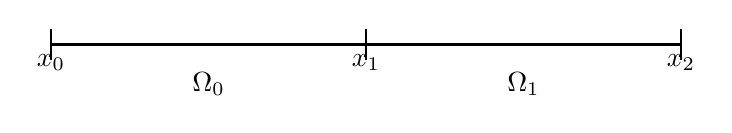
\begin{tikzpicture}
	\draw[thick, black] (0,0) -- (8,0);
	\draw[thick, black] (4,-0.2) --node[below]{$x_1$} (4,0.2);
	\draw[thick, black] (0,-0.2) --node[below]{$x_0$} (0,0.2);
	\draw[thick, black] (8,-0.2) --node[below]{$x_2$} (8,0.2);
	\node at (2,-0.5) {$\Omega_0$};
	\node at (6,-0.5) {$\Omega_1$};
\end{tikzpicture}
\caption{Radial grid showing discontinuous domains $\Omega_0$ and $\Omega_1$.}
\end{figure}
Let's consider elastic collisions, where $v^\prime = (\sqrt{1-\mu})v$ and $\mu=m_e/M \approx 10^{-5}$.
For the domain $\Omega_0$, we can write, 
\begin{align}
	C_{\Omega_0}^{-} &= -v_{th}^4\int_{x0}^{x1} x^3 \sigma f_{l}^{(\Omega_0)}\of{x} T^{(\Omega_0)}\of{x} dx \\
		& -v_{th}^4\int_{x0}^{x0/\sqrt{1-\mu}} x^3 \sigma f_{l}^{(\Omega_0)}\of{x} T^{(\Omega_0)}\of{x} dx -v_{th}^4 \int_{x0/\sqrt{1-\mu}}^{x1}x^3 \sigma f_{l}^{(\Omega_0)}\of{x} T^{(\Omega_0)}\of{x} dx
\end{align}
For the gain term we can write, 
\begin{align}
	C_{\Omega_0}^{+} &= v_{th}^4\int_{x0/\sqrt{1-\mu}}^{x1} x^3 \sigma f_{l}^{(\Omega_0)}\of{x} T^{(\Omega_0)}\of{x^\prime} dx + v_{th}^4\int_{x1}^{x1/\sqrt{1-\mu}} x^3 \sigma f_{l}^{(\Omega_1)}\of{x} T^{(\Omega_0)}\of{x^\prime}dx
\end{align}
For general collision terms with energy threshold is larger than the quadrature grid resolution, we can write, 
\begin{align}
	C_{\Omega_0}^{-} &= -v_{th}^4\int_{x0}^{x1} x^3 \sigma f_{l}^{(\Omega_0)}\of{x} T^{(\Omega_0)}\of{x} dx
\end{align}
\begin{align}
	C_{\Omega_0}^{+} &= v_{th}^4\int_{x0 + \epsilon(x_0)}^{x1 + \epsilon(x_1)} x^3 \sigma f_{l}\of{x} T^{(\Omega_0)}\of{x^\prime} dx
\end{align}




%For the domain $D=[D_l,D_r]$ let $\phi_{k}\of{\frac{v}{v_{th}}}$ be the trial functions for expansion and $\psi_{p}\of{\frac{v}{v_{th}}}$ be the corresponding test functions. Let $f_{lm}(v)=\sum_{k} f_{klm} \phi_k(v)$, then projecting the above to $\psi_p(v)$ and using integration by parts we can write,
%\begin{align*}
%	&\partial_t M^{p}_{k} f_{kqs} -EA^{qs}_{lm}\of{[f_{lm}^*(v) v^2 \psi_{p}\of{v}]_{D_l}^{D^r} -(D^{p}_k + 2S^{p}_{k})f_{klm}} -E B^{qs}_{lm} S^{p}_{k} f_{klm} = C^{pqs}_{klm} f_{klm}  \\
%	&\partial_t M^{p}_{k} f_{kqs} = -E \of{\of{2 A^{qs}_{lm} -B^{qs}_{lm}} S^p_{k} + A^{qs}_{lm} D^{p}_{k}}f_{klm} + C^{pqs}_{klm} f_{klm} + EA^{qs}_{lm}[f_{lm}^*(v) v^2 \boldsymbol{\psi}\of{v}]_{D_l}^{D^r}
%\end{align*} where, 
%The flux term (up-winding) determined by $A^{qs}_{lm}$ sign of the eigenvalues. 
%For the domain $D=[D_l,D_r]$ let $\phi_{k}\of{\frac{v}{v_{th}}}$ be the trial functions for expansion and $\psi_{p}\of{\frac{v}{v_{th}}}$ be the corresponding test functions. Let $y_{lm}(v)=\sum_{k} y_{klm} \phi_k(v)$, then projecting the above to $\psi_p(v)$ we can write, 
%\begin{align*}
%	&\partial_t M^{p}_{k} y_{kqs} -E\Lambda^{qs}_{lm}\of{[y_{lm}^*(v) v^2 \psi_{p}\of{v}]_{D_l}^{D^r} -(D^{p}_k + 2S^{p}_{k})y_{klm}} -E Q^T B^{qs}_{lm} Q S^{p}_{k} y_{klm} = Q^T C^{pqs}_{klm}Q y_{klm}  \\
%	&\partial_t M^{p}_{k} y_{kqs} + E\Lambda^{qs}_{lm}(D^{p}_k + 2S^{p}_{k})y_{klm} -E Q^T B^{qs}_{lm} Q S^{p}_{k} y_{klm} = Q^T C^{pqs}_{klm}Q y_{klm} + E\Lambda[y_{lm}^*(v) v^2 \psi_{p}\of{v}]_{D_l}^{D^r} \\
%	&\partial_t M^{p}_{k} y_{kqs} = -E \of{\of{2 \Lambda^{qs}_{lm} -Q^T B^{qs}_{lm} Q} S^p_{k} + \Lambda^{qs}_{lm} D^{p}_{k}}y_{klm} + Q^T C^{pqs}_{klm}Q y_{klm} + E\Lambda^{qs}_{lm}[y_{lm}^*(v) v^2 \psi_{p}\of{v}]_{D_l}^{D^r}
%\end{align*}
\newpage
\subsection{Using piecewise polynomials}
$P_k\of{t}$ be Chebyshev polynomial with degree $k$, defined on domain $t\in[-1,1]$. For $\of{\frac{v}{v_{th}}} \in [a,b]$, we can write 
\begin{align*}
	x=\of{\frac{v}{v_{th}}} &= \of{\frac{b-a}{2}}t + \of{\frac{a+b}{2}} \\
	\phi_k\of{\frac{v}{v_{th}}} &= \exp\of{-\of{\frac{v}{v_{th}}}^2} P_k(t) \\
	\psi_k\of{\frac{v}{v_{th}}} &= P_k(t) \\
	M^p_k = &\myint_{av_{th}}^{b v_{th}} v^2 \psi_p\of{\frac{v}{v_{th}}} \phi_k\of{\frac{v}{v_{th}}} dv = v_{th}^3  \myint_{a}^{b} x^2 \psi_p\of{x} \phi_k\of{x}dx\\
	&=v_{th}^3 \myint_{-1}^{1} x^2 \exp\of{-x^2}  P_k(t) P_p(t) \of{\frac{b-a}{2}} dt
\end{align*} Where full mass matrix (i.e., with spherical basis)
\begin{align*}
	M^{pqs}_{klm} = M^{p}_k \delta^{q}_{l} \delta^{s}_{m}
\end{align*}


%were $C^{qs}_{lm}$ denotes the projection of the collision operator to $Y_{qs}$, which can be written as, 
%\begin{align*}
%C^{qs}_{lm} &=\myint_{S^2} C Y_{qs}\of{\omega_{v}} \diff{\omega_{v}}= 
%\myint_{R} \myint_{S^2} \myint_{S^2} 
%B_0\of{(v^\prime,\omega_{v}), \vect{\omega}} {v^\prime}^2 Y_{lm}\of{\omega_{v}} \times \\
%\Bigg(
%&\delta\of{v^{post}- {v}} Y_{qs}\of{\omega_{v^{post}}} - \delta\of{v^\prime - v} Y_{qs}\of{\omega_{v}}
%\Bigg)
%\diff{\vect{\omega}} \diff{\vect{\omega_{v_e}}} \diff{v^\prime} 
%\end{align*}
%Let $f_{lm}$ be the lm modes used, 
%\begin{align*}
%\partial_tf_{qs}
%-E A^{qs}_{lm} \partial_v f_{lm}  
%-E B^{qs}_{lm} \frac{1}{v}f_{lm}  = 
%C^{qs}_{lm}f_{lm}
%\end{align*}
%\textbf{Note}: Due to the orthogonality structure in the radial advection coordinate diagonals will always be zero, with a banded matrix with width of equal to 1. 
\clearpage
\section{1D glow discharge problem}
\label{sec:1d_glow}
\textbf{Research Objectives}: 
Establish differences between macroscopic fluid model with closure models for kinetic coefficients vs. fully coupled Boltzmann solver for electron kinetics for the 1d glow discharge problem. 
%in correspondence with the fully coupled 1D2V electron kinetic coefficients determined by the electron-Boltzmann solver.

\subsection{Macroscopic model}
Here we summarize the macroscopic model for the 1D glow discharge problem. Here subscript $s$ denotes the species type (i.e., $s=Ar^{+}, Ar^{*}$) and $k_s$ denotes the corresponding reaction rates. 
\begin{align}
	&\partial_t{n_{s}} + \nabla \cdot \vect{J_{s}} = k_s \of{T_e} n_0 n_e \\
	&\partial_t \of{\frac{3}{2} n_e k T_e} = -\nabla \cdot \vect{q_e} - e \vect{J_e} \cdot \vect{E} - H_ik_i n_0 n_e\\
	& \Delta V = -\frac{e}{\epsilon_0} (n_i-n_e)
\end{align} where 
\begin{align}
	&\vect{J_{s}} = Z_{s} \mu_{s} n_{s} \vect{E} -D_{s} \nabla n_{s} \\
	&\vect{q_e} 	= -\frac{3 k D_e n_e}{2} \nabla T_e + \frac{5}{2} k T_e \vect{J_e} \\
	&k_i\of{T_e}     	    = 1.235 \times 10^{-13} \exp (-18.687 / T_{e})  
\end{align} 
For the 3-species Ar collision model (i.e. $Ar$, $Ar^{+}, e$) boundary conditions are specified as follows. We assume constant $Ar$ density which is denoted by $n_0$.
\begin{align}
	&J_i = \mu_i n_i E \text{ , } J_e = -k_a n_e - \gamma J_i \text{ , } T_{ev} = T_{eb} \text{ , } V = V_0 \sin\of{2\pi f t} \text{ at } x=0\\
	&J_i  = \mu_i n_i E \text{ , } J_e = k_a n_e - \gamma J_i \text{ , } T_{ev} = T_{eb} \text{ , } V = 0 \text{ at } x=L
\end{align} where, $k_a = 1.19 \times 10^{5} ms^{-1}$ denotes the electron recombination coefficient, and $\gamma=0.01$ denotes the secondary electron emission coefficient. We use SI units except for the temperature we use $\text{eV}$.

\textbf{Discretization}: We use chebyshev-collocation spectral method for the spatial discretization. Let $D_x $, $LpD$ be the 1D discretized derivative operators, corresponding $\partial_x$ and $\Delta$ with Dirichlet boundary conditions. Following quantities are important for the right-hand-side (RHS) derivative computations w.r.t. the state variable.  
\begin{align*}
	&\partial_{n_k} J_s = Z_s \mu_s \of{n_s \partial_{n_k}E + E \partial_{n_k}n_s} -Ds D_x  \partial_{n_k}n_s \\
	&\partial_{n_i} V   = LpD^{-1} \frac{\alpha e}{\epsilon_0 V_0} I_{D} \text{ and } \partial_{n_e} V   = -\partial_{n_i} V\\
	&\partial_{n_e} q_e = -\frac{3D_e}{2} D_x T_{ev} I + \frac{5 T_{ev}}{2} \partial_{ne} J_e \\
	&\partial_{T_{ev}} q_e = -\frac{3D_e n_e}{2} D_x + \frac{5}{2} J_e I  \\
	&\partial_{n_k} \of{J_e E} = J_e \partial_{n_k} E + E \partial_{n_k} J_e \\
\end{align*} The above coupled system is evolve with fully implicit Backward Euler time integration. 

\subsection{1D glow discharge with the electron Boltzmann}
We rewrite the 1D glow discharge model, with electron Boltzmann equation as below. 
\begin{align}
	&\partial_t n_s + \nabla \cdot \vect{J_s} = k_s n_0 ne \text{ where } \vect{J_s} = Z_{s} \mu_{s} n_{s} \vect{E} -D_{s} \nabla n_{s}\\
	& \Delta V = -\frac{\alpha e}{\epsilon_0 V_0} (n_i-n_e) \\
	& \partial_t f + \vect{v} \cdot \nabla_{\vect{x}} f -\frac{e}{m_e} \vect{E} \cdot \nabla_{v} f = n_0 C_{en}f + \Gamma(n_0, T_{ev}, n_i) C_{ee} (f, f) 
\end{align} In the above $f: (t, x, v, \vtheta) \mapsto \mathcal{R}^+$ is the electron distribution function. For the 1D glow discharge problem the boundary conditions are given below. 
\begin{align}
	\vect{J_s}(x=0) = \mu_s n_s \vect{E} \text{ and } \vect{J_s}(x=L) = \mu_s n_s \vect{E} \\
	V(x=0) = V_0\sin(2\pi f t) \text{ and } V(x=L) = 0 \\
	f(t, x=0, v, \vtheta \leq \frac{\pi}{2}) = 0 \text{ and } f(t, x=L, v, \vtheta > \frac{\pi}{2}) = 0
\end{align}
\textbf{Discretization}: The electron distribution function $f(t, x, v, \vtheta)$ is discretized as follows. 
\begin{itemize}
	\item $x$ (i.e., physical space) we use Chebyshev-collocation method
	\item $v$ (i.e., radial speed) we use B-Splines with Galerkin approach
	\item we use method of ordinates in $\vtheta$ (i.e., polar angle $\vtheta$ v-space) 
	\item For collision operator and v-space advection we use B-splines + spherical harmonics with Galerkin approach
\end{itemize} 
\begin{align}
	&f(t, x, v, \vtheta) = \sum_{k} f_{k}(t,x,\vtheta) S_k\of{\bar{v}} \text{ where } \bar{v} = \frac{v}{v_{th}} 
\end{align} with $v_{th}$ is the thermal velocity to normalize the radial speed coefficient.
\par \textbf{Spatial advection term}: The Galerkin projection of the spatial advection term can be written as, 
\begin{align*}
	v\cos\of{\vtheta} \partial_x f &= v\cos\of{\vtheta} \sum_{k} \partial_x\of{f_{k}(t,x,\vtheta)} S_k\of{\bar{v}}\\
	\myint_{R} v^3 S_p(\bar{v}) \cos\of{\vtheta} \partial_x f \diff{v} &=\cos\of{\vtheta} A D_x f \text{ where } A_{pk} = {v_{th}}^4 \myint_{R} \bar{v}^3 S_p(\bar{v}) S_k(\bar{v}) \diff{\bar{v}} \\
	M_{pk} &= {v_{th}}^3\myint_{R} \bar{v}^2 S_p(\bar{v}) S_k(\bar{v}) \diff{\bar{v}} \text{ be the mass matrix}
\end{align*} The discretized 1D2V Boltzmann equation can be written as follows. 
\begin{align}
	\of{I_{N_{\vtheta}} \otimes M  } \partial_{t} \vect{f} &= \nonumber\\&P_{so}\of{n_0 C_{en} + \Gamma(n_0, T_{ev}, n_i) C_{ee} (\cdot, \cdot) + \frac{e E}{m_e} A_v} P_{os} \vect{f} \nonumber \\ &- \of{I_{N_{\vtheta}} \otimes \cos\of{\vtheta_j} A D_x  } \vect{f} \label{eq:1d2v_bte}
\end{align} Where $A_v$ denotes the advection operator in v-space, $P_{os}$ denotes the ordinates to spherical harmonic basis projection and $P_{so}$ denotes the spherical to ordinates projection operator. Note that all the v-space operators (i.e., advection, electron-heavy and electron-electron) are discretized using B-spline + spherical harmonic basis with standard Galerkin approach as described previously.

Let $N_p, N_r, N_\vtheta$ and $N_{l}$ be the degrees of freedom used for the space, number of B-splines, number of ordinates, and number of $l$-modes (for v-space operator discretization) used for the discretized $f$ respectively. 

\textbf{Approach I}: Fully implicit integration for the 1D2V scheme, will require dense Jacobian with size $\mathcal{O}(N_r^2 N_\vtheta^2 N_p^2)$ with direct LU factored solve with $\mathcal{O}(N_r^6 N_\vtheta^6 N_p^6)$. One approach might be to use iterative scheme with preconditioning for fast convergence. 

\textbf{Approach II}: Use operator splitting for equation \eqref{eq:1d2v_bte}. The following operator splitting scheme is used for the 1D2V Boltzmann equation. 

\begin{align}
	&\partial_t \vect{f} + \cos\of{\vtheta} M^{-1} A \partial_x \vect{f} = 0 \label{eq:1d2v_x_adv} \\
	&\partial_t \vect{f} =\of{I_{N_{\vtheta}} \otimes M  }^{-1} P_{so}\of{n_0 C_{en} + \Gamma(n_0, T_{ev}, n_i) C_{ee} (\cdot, \cdot) + \frac{e E}{m_e} A_v} P_{os} \vect{f} \label{eq:1d2v_v_space1}
\end{align} For simplicity, we write mass matrix absorbed operators (e.g., $A \equiv M^{-1} A$) unless otherwise specified. Equation \eqref{eq:1d2v_x_adv} is solved analytically, with $A=Q_A \Lambda_A Q_A^{-1}$ diagonalized $A$. Let $\vect{h} = Q_{A}^{-1}\vect{f}$ then we can write the analytical solution as \eqref{eq:bte_x_adv_q1}.
\begin{align}
	\vect{h}(t,\vect{x},\vect{\vtheta}) = \vect{h_0}(\vect{x} - \Lambda\cos(\vect{\vtheta}) t, \vect{\vtheta}) \label{eq:bte_x_adv_q1}
\end{align} Equation \eqref{eq:1d2v_v_space1} solved with fully implicit solver with Newton's method. 
The overall operator splitting scheme is summarized in Algorithm \ref{alg:1dglow_bte_op}.

\begin{algorithm}[!tbhp]
	\caption{Overview for 1D glow discharge with Boltzmann \label{alg:1dglow_bte_op}}
	\begin{algorithmic}[0]
		\Require $n_s(t,x), \vect{f}(t,x)$ and $\Delta t$
		\Ensure $n_s(t + \Delta t, x), \vect{f}(t + \Delta t, x), E(t+\Delta t)$ 
		\State $f_0 \leftarrow \text{advection\_x} (\vect{f}(t))$
		\State $f_1 \leftarrow \text{boltzmann\_v\_solve} (f_0) $
		\State $n_e(t, x), k_i(t, x) \leftarrow \text{boltzmann\_to\_fluid}(f_1)$ 
		\State $n_s(t + \Delta t), E(t+\Delta t) \leftarrow \text{fluid\_solve}(n_s, n_e, k_i, t = t, dt=\Delta t)$
		%\State $E(t+\Delta t) \leftarrow \text{fluid\_to\_boltzmann}()$ 
		\State \Return $n_s(t + \Delta t, x), f_1, E(t+\Delta t)$ 
	\end{algorithmic}
\end{algorithm}

\subsection{Implicit-Explicit methods}
In this section we explore implicit-explicit (IMEX) schemes for 1D glow discharge problem. Let's consider the ODE given by \eqref{eq:imex_ode}. Here $F$ and $G$ denotes the operators that handled explicitly and implicitly respectively. The implicit-explicit Runge-Kutta (IMEX-RK) scheme is given by \eqref{eq:imex_rk}.
\begin{align}
	&\dot{U} + F(U) + G(U) = 0 \label{eq:imex_ode}\\
	&U^{i} = U^n + \Delta t \sum_{j=1}^{i-1} \hat{A}_{ij} F\of{U^j} + \Delta t \sum_{j=1}^{i} A_{ij} G\of{U^{j}} \\
	&U^{n+1} = U^{n} + \Delta t \sum_{i=1}^{s} \hat{b}_i F\of{U^i} + \Delta t \sum_{i=1}^{s} b_i G\of{U^i} \label{eq:imex_rk}
\end{align}
For 1D glow discharge problem, we can treat x-space advection implicitly with all the other terms are treated explicitly. 
\begin{align}
	&\partial_t n_s + \underbrace{\nabla \cdot \vect{J_s}}_{\text{implicit}} = \underbrace{S(f, n_0)}_{explicit}\\
	&\partial_t f    + \underbrace{\cos(\vtheta) A_x \partial_x f}_{\text{implicit}} = \underbrace{C(f, T_g, n_s) + A_v f}_{explicit} \\
	&E = \frac{e}{\epsilon} (n_i - n_e)
\end{align}
In the above, we get a decoupled system that where the operators can be inverted during the setup phase. 



% \noindent $n$ ions, $f$ electrons, $E$ electric field;\\
% Here I asume $\delta t =1$ for notational simplicity.\\
% I also use an Euler scheme. \\
% $p$ subscript means the solution at $t+\delta t$\\
% $s(f)$ are terms from $f$ to $n$.
% $J$ is the ion flux
% \begin{align}
% 	&f_p + v \partial_x f_p = E \partial_v f + C(f)\\
% 	&n_p + \nabla \cdot J(E,n_p) = s(f)\\
% 	&E_p = -\nabla \Delta^{-1} \left(n-\int_v f\right)
% \end{align}
% \noindent Essentially, the left hand side has three block, linear implicit solves\\
% The right hand side are explicit terms\\
% We should use Crank-Nicolson for implicit; and RK2 for explicit.

\ \ 
\newpage
\newpage
\subsection{Old notes on 1D glow discharge}
We can write the Boltzmann equation in full 7d case as below. 
\begin{align*}
\partial_t f + \vect{v}\cdot \nabla_{\vect{x}} f -\frac{q}{m} \vect{E} \cdot \nabla_{\vect{v}} f = C[f]
\end{align*}
Based on the above we derive the governing equations for the 1d glow-discharge problem. We apply time varying voltage in the $\vect{\hat{z}}$ direction which result in a time varying electric filed. Let $\Omega_z=(0, L)$ , $\Omega_v= \mathcal{R}^3$ be the space and velocity domains. For $(z, v) \in \Omega_{z} \times \Omega_v$ where $f (v, z, t) : \Omega_{v} \times \Omega_{z} × [0,T] \rightarrow \mathcal{R}^{+}$ be the electron distribution function. The governing equations for the scalar potential V corresponding to the electric field can be written as,
\begin{align*}
	\Delta V = -\frac{e}{\epsilon_0} (n_i-n_e) \text{ where } n_e(z,t) = \myint_{\vect{v}} f(\vect{v}, z, t) \diff{\vect{v}} \\
	V(0,t) = V_0 \sin(2\pi ft) \text{ , } V(L,t) = 0 \text{ and } \vect{E} = E \vect{\hat{z}} = -\of{\partial_z V} \vect{\hat{z}}
\end{align*} 

\par The ionized heavy densities are governed by the drift-diffusion equation below.
\begin{align*}
	&\partial_t n_i + \partial_z J_i = k_i n_0 n_e \text{ where } J_i\of{z, t} = \mu_i n_i E\of{z,t} -D_i \partial_z n_i\\
	&J_i(z,t)=\max\of{\mu_i n_i \vect{E}\cdot \vect{\hat{n}},0} \text{ for } z =0 \text{ and } z=L
\end{align*} With finite volume discretization we can write, 
\begin{align}
	\partial_t n_i + \frac{1}{\Delta z_m} \of{J\of{z_{m+1/2},t} - J\of{z_{m-1/2},t}} = \frac{1}{\Delta z_m}  \myint_{z_{m-1/2}}^{z_{m+1/2}} k_i n_0 n_e dz
\end{align} We currently use central linear flux reconstruction method where flux function at the boundary computed as below. 
\begin{align*}
&J\of{z_{m+1/2}} = \mu_i \frac{\of{n_{i,m+1} + n_{i,m}}}{2} \frac{\of{V_m-V_{m+1}}}{\Delta z_m} - D_i \frac{\of{n_{i, m+1} -n_{i, m}}}{\Delta z_m} \\
&J\of{z_{m-1/2}} = \mu_i \frac{\of{n_{i,m} + n_{i,m-1}}}{2} \frac{\of{V_{m-1}-V_{m}}}{\Delta z_m} - D_i \frac{\of{n_{i, m} -n_{i, m-1}}}{\Delta z_m} \\
&\frac{1}{\Delta z_m}  \myint_{z_{m-1/2}}^{z_{m+1/2}}  k_i n_0 n_e dz \approx k_{i,m} n_{0,m} n_{e,m} 
\end{align*}

The electron densities are governed by the Boltzmann equation below. 
\begin{align*}
&	\partial_t f + v\cos\of{\vtheta} \partial_z f -\vect{E}\cdot\nabla_v f = C[f] \text{ for } (z,\vect{v}) \in (0,L) \times[0,v_{max}]^3 \\
& f(\vect{v}, 0, t, \vtheta \leq \frac{\pi}{2})	= 0 \text{ and } f(\vect{v}, L, t, \vtheta > \frac{\pi}{2})	= 0
\end{align*}
We need to specify the boundary conditions depending on the sign of $v \cos\vtheta$.

\subsection{Discretizing in polar angle ($\vtheta$)}
In order to resolve the boundary conditions, we discretize f , radially with B-splines with basis $\{S_k\of{\frac{v}{\vth}}\}_{k=0}^{N_r}$ regular grid discretization with collocation method in $\vtheta$ and $z$ directions. 

Let $\{\vtheta\}_{j=0}^{N_\vtheta}$ be the points in the $\vtheta$ direction, for each $\vtheta_j$ we use the B-spline expansion. 
\begin{align*}
	&f(v, \vtheta_j , z, t) = f_{\vtheta_j} (v, z, t) = \sum_k f_{\vtheta_j, k} \of{z,t} S_k\of{\frac{v}{\vth}} \\
	& \partial_z f = \sum_{k} S_k\of{\frac{v}{\vth}} \partial_z f_{\vtheta_j, k} \\
	& v\cos\of{\vtheta_j} \partial_z  = v\cos\of{\vtheta_j} \sum_{k} S_k\of{\frac{v}{\vth}} \partial_z f_{\vtheta_j, k}
\end{align*} Projecting the above onto radial direction test basis functions $T_p\of{\frac{v}{\vth}}$, we can write, 
\begin{align*}
&\myint_v T_p \of{\frac{v}{\vth}} v^3 \cos\of{\vtheta_j} \partial_z f dv = \myint_v T_p \of{\frac{v}{\vth}} v^3\cos\of{\vtheta_j} \sum_{k} S_k\of{\frac{v}{\vth}} \partial_z f_{\vtheta_j, k} dv \\
&=\cos\of{\vtheta_j} \sum_k \myint_v v^3 T_p\of{\frac{v}{\vth}} S_k\of{\frac{v}{\vth}} dv \partial_z f_{\vtheta_j,k} = \cos\of{\vtheta_j} W^{p}_{k} D_z f_{\vtheta_j,k}
\end{align*} where $D_z$ is upwinded finite derivative stencil based on $\vtheta_j$. We write the discretize operators, 
\begin{align*}
W^{p}_{k} = \myint_v v^3 T_p\of{\frac{v}{\vth}} S_k\of{\frac{v}{\vth}} dv \text{ and }
M^{p}_{k} = \myint_v v^2 T_p\of{\frac{v}{\vth}} S_k\of{\frac{v}{\vth}} dv
\end{align*} 

Currently we assume $l=0, 1$ and $m=0$ modes for the velocity space approximation. For each radial component, we can compute the projection on to the spherical basis, 
\begin{align*}
&	f_k\of{\vtheta,z,t} = \sum_l f_{lk}\of{z, t} Y_{l0}\of{\vtheta}\\
&	f_{lk} = 2\pi \myint_{\vtheta} \sin\of{\vtheta} f_k\of{\vtheta, z, t} Y_{l0} d\vtheta \\
&\sum_{\vtheta_j} w_{\vtheta_j} f_{\vtheta_j,k} Y_{l0}\of{\vtheta_j} = P^{\vtheta_j}_l f_{\vtheta_j,k}
\end{align*} and we can write, 
\begin{align*}
	f_k\of{\vtheta_j, z, t} = f_{\vtheta_j,k} = \sum_l f_{lk}\of{z,t} Y_{l0}\of{\vtheta_j} = Y^{l}_{\vtheta_j} f_{lk}
\end{align*}
Let $E^{pq}_{kl}$ and $C^{pq}_{kl}$ be the Galerkin discretization of V-space advection and collision operators. Then we can write the full 1d Boltzmann equation discretized, 
\begin{align*}
\of{I_{N_\vtheta} \otimes M^{p}_{k}} \partial_t f_{\vtheta_j, k , z, t} + \of{I_{N_\vtheta} \otimes \of{\cos\of{\vtheta_j} W^{p}_k D_z}} f_{\vtheta_j, k , z, t} \\
= Y_{\vtheta_j, q} (E^{pq}_{kl} + C^{pq}_{kl}) \of{P^{\vtheta_j}_{l} f_{\vtheta_j,k,z,t}}^{T}
\end{align*}

Let $f\equiv f\of{t, v, \vtheta, z}$, and we can write, 
\begin{align*}
	\vect{E} 
	= E \hat{\vect{z}} 
	= E \left( \cos\of{\vtheta} \vrunit - \sin\of{\vtheta} \vthetaunit \right)
\end{align*}
\begin{align*}
	\vect{E}\cdot \nabla_{\vect{v}} f
	= E 
	\left( \cos\of{\vtheta} \frac{\partial f}{\partial \vr} 
	- \sin\of{\vtheta} \frac{1}{\vr} \frac{\partial f}{\partial \vtheta} \right)
\end{align*}

\begin{align*}
&\partial_t f + v\cos\of{\vtheta} \partial_z f -\vect{E}\cdot\nabla_v f = C[f] \\
&\implies \partial_t f + v\cos\of{\vtheta} \partial_z f -\frac{Eq}{m} 
\left( \cos\of{\vtheta} \frac{\partial f}{\partial \vr} 
- \sin\of{\vtheta} \frac{1}{\vr} \frac{\partial f}{\partial \vtheta} \right) = C[f] 
\end{align*}







\clearpage
\subsection{Advection + Collision operator}
This section attempt to understand collective effect on advection + collision operators. For simplicity of the analysis, we assume we use $l=0,1$ polar and $m=0$ in the azimuthal direction. We use $S_k\of{x}$, $T_p\of{x}$ to denote trial and test basis respectively. Important coordinate relations are listed below. 
\begin{align*}
x =\frac{v_r}{v_{th}} \text{, } \varepsilon = \of{\frac{v_r}{\gamma}}^2 \text{ where } \gamma = \sqrt{2 e / m_e}
\end{align*}
Recall, the simplified collision operator projected on to spherical harmonics can be written as follows. 
\begin{align*}
C^{q}_{l} &= \myint_{R} {v^\prime_r}^2 B(v^\prime_r) f_l \delta_{ql}\of{\delta\of{v^{post}(v^\prime_r)-v_r} \delta_{q0} - \delta\of{v^\prime_r -v_r}} \diff{v^\prime_r}
\end{align*} We can write the collision operator with advection terms, 
\begin{align*}
\partial_t M^{q}_{l} f_{l}
-E A^{q}_{l} \partial_{v_r} f_{l}  
-E B^{q}_{l} \frac{1}{v_r}f_{l}  = 
C^{q}_{l}f_{l}
\end{align*} Now with expanding each radial component with trial basis and projecting it onto the test space we can write, 
\begin{align*}
f_l\of{v_r} &= \sum_{k} f_{kl} S_k(x) 
\end{align*}
\begin{align*}
\partial_t M^{pq}_{kl} f_{kl} = -\of{\of{2 A^{q}_{l} -B^{q}_{l}} W^p_{k} + A^{q}_{l} D^{p}_{k}}f_{kl} + C^{pq}_{kl} f_{kl} + EA^{q}_{l}[f_{l}^*(v) v^2 \boldsymbol{T}\of{v}]_{D_l}^{D^r}
\end{align*}Where, 
\begin{align*}
M^{pq}_{kl} &= v_{th}^3 \myint_{R} x^2 T_p \of{x} S_k\of{x} dx \\
W^{p}_{k}   &= v_{th}^2 \frac{E q}{m_e} \myint_{R} x T_p \of{x} S_k\of{x} dx \\
D^{p}_{k}   &= v_{th}^2 \frac{E q}{m_e} \myint_{R} x^2 \partial_x T_p \of{x} S_k\of{x} dx \\
A^{q}_{l} &=\begin{pmatrix}
0  & 1/\sqrt{3} \\
1/\sqrt{3}  & 0 \\
\end{pmatrix} \text{ , } 
B^{q}_{l} = \begin{pmatrix}
0 & 2/\sqrt{3}\\
0 & 0 
\end{pmatrix}\\
C^{pq}_{kl} &= \begin{pmatrix}
C^{p0}_{k0} & 0 \\
0  & C^{p1}_{k1} \\
\end{pmatrix}\text{where, } \\
C^{p0}_{k0}  &= -n_0 v_{th}^4 \frac{\mu}{2} \myint_{R} x^4 \sigma\of{\varepsilon} S_k\of{x}\partial_{x} T_p\of{x} \diff{x}  \\
C^{p1}_{k1}  &= -n_0 v_{th}^4 \myint_{R} x^3 \sigma\of{\varepsilon} S_k\of{x} T_p\of{x} \diff{x} 
\end{align*}






\clearpage
\section{Advection term}
\subsection{Eulerian approach}
Advection (acceleration) term
\begin{align*}
\partial_t f + \vect{E}\cdot \nabla_{\vect{v}} f = C[f]
\end{align*}
In spherical coordinates
\begin{align*}
\nabla_{\vect{v}} 
= \vrunit \frac{\partial}{\partial \vr}
+ \vthetaunit \frac{1}{\vr} \frac{\partial}{\partial \vtheta}
+ \vphiunit \frac{1}{\vr \sin\of{\vtheta}} \frac{\partial}{\partial \vphi}
\end{align*}
\begin{align*}
\vect{E} 
= E \hat{\vect{z}} 
= E \left( \cos\of{\vtheta} \vrunit - \sin\of{\vtheta} \vthetaunit \right)
\end{align*}
\begin{align*}
\vect{E}\cdot \nabla_{\vect{v}} f
= E 
\left( \cos\of{\vtheta} \frac{\partial f}{\partial \vr} 
- \sin\of{\vtheta} \frac{1}{\vr} \frac{\partial f}{\partial \vtheta} \right)
\end{align*}
Expansion in terms of Maxwell polynomials and spherical harmonics
\begin{align*}
f = 
\sum_{klm} a_{klm} \Phi_{kl}\of{\frac{v}{\vth}} Y_{lm}\of{\vtheta,\vphi}
\end{align*}
Spherical harmonics
\begin{align*}
Y_{lm}\of{\vtheta,\vphi} = U_{lm} P^{|m|}_l\of{\cos\of{\vtheta}} \alpha_m\of{\vphi}
\end{align*}
\begin{align*}
U_{lm} &= 
\begin{cases}
(-1)^m \sqrt{2} \sqrt{\frac{2l+1}{4\pi} \frac{(l-|m|)!}{(l+|m|!}}, &m\neq 0 \\
\sqrt{\frac{2l+1}{4\pi}}, &m = 0
\end{cases}
\\
\alpha_m\of{\vphi}
&=
\begin{cases}
\sin\of{|m|\phi}, &m < 0 \\
1, &m = 0\\
\cos\of{m\phi}, &m > 0
\end{cases}
\end{align*}
Useful relationships
\begin{align*}
x P^m_l\of{x} 
&= \frac{l+m}{2l+1} P^m_{l-1}\of{x}
+ \frac{l-m+1}{2l+1} P^m_{l+1}\of{x}
\\
&= \alpha_M\of{l,m} P^m_{l-1}\of{x}
+ \beta_M\of{l,m} P^m_{l+1}\of{x}
\\
(1-x^2) \frac{d}{dx} P^m_l\of{x} 
&= \frac{(l+1)(l+m)}{2l+1} P^m_{l-1}\of{x} 
- \frac{l(l-m+1)}{2l+1} P^m_{l+1}\of{x}
\\
&= \alpha_D\of{l,m} P^m_{l-1}\of{x} 
+ \beta_D\of{l,m} P^m_{l+1}\of{x}
\end{align*}
Now we can show
\begin{align*}
\cos\of{\vtheta} Y_{lm}\of{\vtheta,\vphi}
&=
\cos\of{\vtheta} U_{lm} P^{|m|}_l\of{\cos\of{\vtheta}} \alpha_m\of{\vphi}
\\
&=
\cos\of{\vtheta} U_{lm} P^{|m|}_l\of{\cos\of{\vtheta}} \alpha_m\of{\vphi}
\\
&=
U_{lm} \left( \alpha_M\of{l,|m|} P^{|m|}_{l-1}\of{\cos\of{\vtheta}} 
+ \beta_M\of{l,|m|} P^{|m|}_{l-1}\of{\cos\of{\vtheta}} \right) \alpha_m\of{\vphi}
\\
&=
\alpha_M\of{l,|m|} \frac{U_{lm}}{U_{(l-1)m}} Y_{(l-1)m}\of{\vtheta,\vphi} 
+ \beta_M\of{l,|m|} \frac{U_{lm}}{U_{(l+1)m}} Y_{(l+1)m}\of{\vtheta,\vphi}
\\
&=
A_M\of{l,m} Y_{(l-1)m}\of{\vtheta,\vphi} 
+ 
B_M\of{l,m} Y_{(l+1)m}\of{\vtheta,\vphi}
\end{align*}

\begin{align*}
-\sin\of{\vtheta} \frac{d}{d\vtheta} Y_{lm}\of{\vtheta,\vphi}
&=
-\sin\of{\vtheta} U_{lm} \frac{d}{d\vtheta} P^{|m|}_l\of{\cos\of{\vtheta}} \alpha_m\of{\vphi}
\\
&=
\left(\sin\of{\vtheta}\right)^2 U_{lm} \frac{d}{d\cos\of{\vtheta}} P^{|m|}_l\of{\cos\of{\vtheta}} \alpha_m\of{\vphi}
\\
&=
\left(1 - \left(\cos\of{\vtheta}\right)^2\right) U_{lm} \frac{d}{d\cos\of{\vtheta}} P^{|m|}_l\of{\cos\of{\vtheta}} \alpha_m\of{\vphi}
\\
&=
U_{lm} \left( \alpha_D\of{l,|m|} P^{|m|}_{l-1}\of{\cos\of{\vtheta}} 
+ \beta_D\of{l,|m|} P^{|m|}_{l-1}\of{\cos\of{\vtheta}} \right) \alpha_m\of{\vphi}
\\
&=
\alpha_D\of{l,|m|} \frac{U_{lm}}{U_{(l-1)m}} Y_{(l-1)m}\of{\vtheta,\vphi} 
+ \beta_D\of{l,|m|} \frac{U_{lm}}{U_{(l+1)m}} Y_{(l+1)m}\of{\vtheta,\vphi}
\\
&=
A_D\of{l,m} Y_{(l-1)m}\of{\vtheta,\vphi} 
+ 
B_D\of{l,m} Y_{(l+1)m}\of{\vtheta,\vphi}
\end{align*}
Substituting into advection term
\begin{align*}
\vect{E}\cdot \nabla_{\vect{v}} f
&= E 
\left( \cos\of{\vtheta} \frac{\partial f}{\partial \vr} 
- \sin\of{\vtheta} \frac{1}{\vr} \frac{\partial f}{\partial \vtheta} \right)
\\
&= E 
\sum_{klm} a_{klm} 
\Bigg(
\frac{d}{d\vr}\Phi_{kl}\of{\frac{v}{\vth}}
\left( A_M\of{l,m} Y_{(l-1)m}\of{\vtheta,\vphi} 
+ B_M\of{l,m} Y_{(l+1)m}\of{\vtheta,\vphi} \right)
\\
&+
\frac{1}{\vr}\Phi_{kl}\of{\frac{v}{\vth}}
\left( A_D\of{l,m} Y_{(l-1)m}\of{\vtheta,\vphi} 
+ B_D\of{l,m} Y_{(l+1)m}\of{\vtheta,\vphi} \right) 
\Bigg)
\\
&= E 
\sum_{klm} a_{klm} 
\Bigg(
\left( A_M\of{l,m} \frac{d}{d\vr}\Phi_{kl}\of{\frac{v}{\vth}} 
+ A_D\of{l,m} \frac{1}{\vr}\Phi_{kl}\of{\frac{v}{\vth}} \right)
Y_{(l-1)m}\of{\vtheta,\vphi} 
\\
&+
\left( B_M\of{l,m} \frac{d}{d\vr}\Phi_{kl}\of{\frac{v}{\vth}} 
+ B_D\of{l,m} \frac{1}{\vr}\Phi_{kl}\of{\frac{v}{\vth}} \right)
Y_{(l+1)m}\of{\vtheta,\vphi} 
\Bigg)
\end{align*}
Projecting onto test functions
\begin{multline*}
\myint \vect{E}\cdot \nabla_{\vect{v}} f \Psi_{pq}\of{\textstyle\frac{\vr}{\vth}} Y_{qs}\of{\theta,\phi} 
\vr^2 \diff{\vr} \diff{\vomega}\\
= E 
\myint 
\sum_{k}
\Bigg(
a_{k(q+1)s} 
\left( A_M\of{q+1,s} \frac{d}{d\vr}\Phi_{k(q+1)}\of{\frac{v}{\vth}} 
+ A_D\of{q+1,s} \frac{1}{\vr}\Phi_{k(q+1)}\of{\frac{v}{\vth}} \right)
\\
+ a_{k(q-1)s} \left( B_M\of{q-1,s} \frac{d}{d\vr}\Phi_{k(q-1)}\of{\frac{v}{\vth}} 
+ B_D\of{q-1,s} \frac{1}{\vr}\Phi_{k(q-1)}\of{\frac{v}{\vth}} \right)
\Bigg)
\Psi_{pq}\of{\textstyle\frac{\vr}{\vth}}
\vr^2 \diff{\vr}
\end{multline*}
Non-dimensionalizing integrands
\begin{multline*}
= E \vth^2
\myint 
\sum_{k}
\Bigg(
a_{k(q+1)s} 
\left( A_M\of{q+1,s} \frac{d}{dx}\Phi_{k(q+1)}\of{x} 
+ A_D\of{q+1,s} \frac{1}{x}\Phi_{k(q+1)}\of{x} \right)
\\
+ a_{k(q-1)s} \left( B_M\of{q-1,s} \frac{d}{dx}\Phi_{k(q-1)}\of{x} 
+ B_D\of{q-1,s} \frac{1}{x}\Phi_{k(q-1)}\of{x} \right)
\Bigg)
\Psi_{pq}\of{x}
x^2 \diff{x}
\end{multline*}
Differentiating by parts
\begin{multline*}
= E \vth^2
\myint 
\sum_{k}
\Bigg(
a_{k(q+1)s} \Bigg( 
\left( A_M\of{q+1,s} - \frac12 A_D\of{q+1,s} \right) 
\Psi_{pq}\of{x} \frac{d}{dx}\Phi_{k(q+1)}\of{x} 
\\
- \frac12 A_D\of{q+1,s} \Phi_{k(q+1)}\of{x} \frac{d}{dx} \Psi_{pq}\of{x} \Bigg)
\\
+ a_{k(q-1)s} \Bigg( 
\left( B_M\of{q-1,s} - \frac12 B_D\of{q-1,s} \right) \Psi_{pq}\of{x} \frac{d}{dx}\Phi_{k(q-1)}\of{x} 
\\
- \frac12 B_D\of{q-1,s} \Phi_{k(q-1)}\of{x} \frac{d}{dx}\Psi_{pq}\of{x}
\Bigg)
\Bigg)
x^2 \diff{x}
\end{multline*}
Writing in a more compact form
\begin{multline*}
= E \vth^2 \sum_{k}
a_{k,q+1,s} \Bigg( 
\left( A_M\of{q+1,s} - \frac12 A_D\of{q+1,s} \right) 
C^{q,\Psi d\Phi+}_{p,k} 
- \frac12 A_D\of{q+1,s} C^{q,\Phi d\Psi+}_{p,k} \Bigg)
\\
+ E \vth^2 \sum_{k}
a_{k,q-1,s} \Bigg( 
\left( B_M\of{q-1,s} - \frac12 B_D\of{q-1,s} \right) C^{q,\Psi d\Phi-}_{p,k}
- \frac12 B_D\of{q-1,s} C^{q,\Phi d\Psi-}_{p,k}
\Bigg)
\end{multline*}
where
\begin{align*}
C^{q,\Psi d\Phi+}_{p,k} 
&= \myint \Psi_{p,q}\of{x} \frac{d}{dx} \Phi_{k,q+1}\of{x} x^2 \diff{x}
\\
C^{q,\Psi d\Phi-}_{p,k} 
&= \myint \Psi_{p,q}\of{x} \frac{d}{dx} \Phi_{k,q-1}\of{x} x^2 \diff{x}
\\
C^{q,\Phi d\Psi+}_{p,k} 
&= \myint \Phi_{k,q+1}\of{x} \frac{d}{dx} \Psi_{p,q}\of{x} x^2 \diff{x}
\\
C^{q,\Phi d\Psi-}_{p,k} 
&= \myint \Phi_{k,q-1}\of{x} \frac{d}{dx} \Psi_{p,q}\of{x} x^2 \diff{x}
\end{align*}
Potentially these can be found analytically and tried to do that for Laguerre polynomials but the results are quite messy. So, it seems to be more convenient just to compute those numerically.

\subsubsection{Case of Maxwell polynomials}

\begin{align*}
\Phi_{kl}\of{x} &= e^{-x^2} x^l \maxp{2l+2}{k}\of{x} \\
\Psi_{pq}\of{x} &= x^q \maxp{2q+2}{p}\of{x} 
\end{align*}

\begin{align*}
\myint_0^\infty \Phi_{kq}\of{x} \Psi_{pq}\of{x} x^2 \diff{x} 
&= \myint_0^\infty e^{-x^2} x^{2q+2}\maxp{2q+2}{k}\of{x} \maxp{2q+2}{p}\of{x} \diff{x}
= \delta_{k,p}
\end{align*}

\begin{align*}
\Psi_{p,q}\of{x} \frac{d}{dx} \Phi_{k,q+1}\of{x} 
&= e^{-x^2} x^{2q} \maxp{2q+2}{p}\of{x} 
\left( \left( (q+1) - 2x^2 \right) \maxp{2q+4}{k} + x \sum_{j=0}^{k-1} \diffm{2q+4}{j}{k} \maxp{2q+4}{j} \right)
\\
\Psi_{p,q}\of{x} \frac{d}{dx} \Phi_{k,q-1}\of{x} 
&= e^{-x^2} x^{2q-2} \maxp{2q+2}{p}\of{x} 
\left( \left( (q-1) - 2x^2 \right) \maxp{2q}{k} + x \sum_{j=0}^{k-1} \diffm{2q}{j}{k} \maxp{2q}{j} \right)
\\
\Phi_{k,q+1}\of{x} \frac{d}{dx} \Psi_{p,q}\of{x}
&= e^{-x^2} x^{2q} \maxp{2q+4}{k}\of{x} 
\left( q \maxp{2q+2}{p} + x \sum_{j=0}^{p-1} \diffm{2q+2}{j}{p} \maxp{2q+2}{j} \right)
\\
\Phi_{k,q-1}\of{x} \frac{d}{dx} \Psi_{p,q}\of{x}
&= e^{-x^2} x^{2q-2} \maxp{2q}{k}\of{x} 
\left( q \maxp{2q+2}{p} + x \sum_{j=0}^{p-1} \diffm{2q+2}{j}{p} \maxp{2q+2}{j} \right)
\end{align*}
where differentiation  matrices
\begin{align*}
\frac{d}{dx} \maxp{l}{k} \of{x} &= \sum_{j=0}^{k-1} \diffm{l}{j}{k} \maxp{l}{j}\of{x}
\end{align*}
are assembled as
\begin{align*}
\diffm{l}{k-1}{k} &= \frac{k}{\beta^{(l)}_k}
\\
\diffm{l}{k-2}{k} &= \frac{\sum_{j=0}^{k-1} \alpha^{(l)}_j - k \alpha^{(l)}_{k-1}}{\sqrt{\beta^{(l)}_k \beta^{(l)}_{k-1}}} 
\\
\diffm{l}{k-3}{k} &= \frac{2 \sqrt{\beta^{(l)}_{k-1} \beta^{(l)}_{k}} - \sqrt{\beta^{(l)}_{k-1}} \diffm{l}{k-1}{k} - \alpha^{(l)}_{k-2} \diffm{l}{k-2}{k} }{\sqrt{\beta^{(l)}_{k-2}}} 
\\
\diffm{l}{j}{k} &= -\frac{\sqrt{\beta^{(l)}_{j+2}} \diffm{l}{j+2}{k} + \alpha^{(l)}_{j+1} \diffm{l}{j+1}{k} }{\sqrt{\beta^{(l)}_{j+1}}}
,\quad 0 \leq j \leq k-4 
\end{align*}

\subsubsection{Case of Laguerre polynomials}
\begin{align*}
\Phi_{kl}\of{x} &= e^{-x^2} x^l \lagp{l+1/2}{k}\of{x^2} \\
\Psi_{pq}\of{x} &= x^q \lagp{q+1/2}{p}\of{x^2} 
\end{align*}

\begin{align*}
\frac{d}{dx} \lagp{l}{k} \of{x^2} 
&= 2 x \frac{d}{dx^2} \lagp{l}{k}\of{x^2} = - 2 x \lagp{l+1}{k-1}\of{x^2}
\end{align*}

\begin{align*}
\Psi_{p,q}\of{x} \frac{d}{dx} \Phi_{k,q+1}\of{x} 
&= e^{-x^2} x^{2q} \lagp{q+1/2}{p} 
\left( \left( (q+1) - 2x^2 \right) \lagp{q+3/2}{k} - 2x^2 \lagp{q+5/2}{k-1} \right)
\\
\Psi_{p,q}\of{x} \frac{d}{dx} \Phi_{k,q-1}\of{x} 
&= 
e^{-x^2} x^{2q-2} \lagp{q+1/2}{p} 
\left( \left( (q-1) - 2x^2 \right) \lagp{q-1/2}{k} - 2x^2 \lagp{q+1/2}{k-1} \right)
\\
\Phi_{k,q+1}\of{x} \frac{d}{dx} \Psi_{p,q}\of{x}
&= e^{-x^2} x^{2q} \lagp{q+3/2}{k} 
\left( q \lagp{q+1/2}{p} - 2x^2 \lagp{q+3/2}{p-1} \right)
\\
\Phi_{k,q-1}\of{x} \frac{d}{dx} \Psi_{p,q}\of{x}
&= e^{-x^2} x^{2q-2} \lagp{q-1/2}{k}
\left( q \lagp{q+1/2}{p} - 2x^2 \lagp{q+3/2}{p-1} \right)
\end{align*}



\subsubsection{Case of Maxwell polynomials in energy}

\begin{align*}
\Phi_{kl}\of{x} &= e^{-x^4} x^l \sqrt{2} \maxp{l+1/2}{k}\of{x^2} \\
\Psi_{pq}\of{x} &= x^q \sqrt{2} \maxp{q+1/2}{p}\of{x^2} 
\end{align*}

\begin{align*}
\myint_0^\infty \Phi_{kq}\of{x} \Psi_{pq}\of{x} x^2 \diff{x} 
&= 2 \myint_0^\infty e^{-x^4} x^{2q+2}\maxp{q+1/2}{k}\of{x^2} \maxp{q+1/2}{p}\of{x^2} \diff{x} 
\\
&= \myint_0^\infty e^{-y^2} x^{q+1/2}\maxp{q+1/2}{k}\of{y} \maxp{q+1/2}{p}\of{y} \diff{y}
= \delta_{k,p}
\end{align*}

\begin{align*}
\frac{d}{dx} \Phi_{k,q} \of{x} 
&= 
\frac{d}{dx} \left( e^{-x^4} x^q \right) \sqrt{2} \maxp{q+1/2}{k}\of{x^2}
+ \left( e^{-x^4} x^q \right) \sqrt{2} 2 x \frac{d}{dx^2} \maxp{q+1/2}{k}\of{x^2}
\\
&= 
e^{-x^4} x^{q-1} \left( q - 4 x^4 \right) \sqrt{2} \maxp{q+1/2}{k}\of{x^2}
+ \left( e^{-x^4} x^q \right) \sqrt{2} 2 x \sum_{j=0}^{k-1} \diffm{q+1/2}{j}{k} \maxp{q+1/2}{j}\of{x^2}
\\
&= 
e^{-x^4} x^{q-1} \sqrt{2} \left( \left( q - 4 x^4 \right) \maxp{q+1/2}{k}\of{x^2}
+ 2 x^2 \sum_{j=0}^{k-1} \diffm{q+1/2}{j}{k} \maxp{q+1/2}{j}\of{x^2} \right)
\end{align*}


\begin{align*}
\frac{d}{dx} \Psi_{k,q} \of{x} 
&= 
\frac{d}{dx} \left(  x^q \right) \sqrt{2} \maxp{q+1/2}{k}\of{x^2}
+ \left( x^q \right) \sqrt{2} 2 x \frac{d}{dx^2} \maxp{q+1/2}{k}\of{x^2}
\\
&= 
x^{q-1} q \sqrt{2} \maxp{q+1/2}{k}\of{x^2}
+ \left( x^q \right) \sqrt{2} 2 x \sum_{j=0}^{k-1} \diffm{q+1/2}{j}{k} \maxp{q+1/2}{j}\of{x^2}
\\
&= 
x^{q-1} \sqrt{2} \left( q \maxp{q+1/2}{k}\of{x^2}
+ 2 x^2 \sum_{j=0}^{k-1} \diffm{q+1/2}{j}{k} \maxp{q+1/2}{j}\of{x^2} \right)
\end{align*}

\begin{align*}
\Psi_{p,q}\of{x} \frac{d}{dx} \Phi_{k,q+1}\of{x} 
&= 2 e^{-x^4} x^{2q} \maxp{q+1/2}{p}\of{x^2} \left( \left( q+1 - 4 x^4 \right) \maxp{q+3/2}{k}\of{x^2}
+ 2 x^2 \sum_{j=0}^{k-1} \diffm{q+3/2}{j}{k} \maxp{q+3/2}{j}\of{x^2} \right)
\\
\Psi_{p,q}\of{x} \frac{d}{dx} \Phi_{k,q-1}\of{x} 
&= 
2 e^{-x^4} x^{2q-2} \maxp{q+1/2}{p}\of{x^2} \left( \left( q-1 - 4 x^4 \right) \maxp{q-1/2}{k}\of{x^2}
+ 2 x^2 \sum_{j=0}^{k-1} \diffm{q-1/2}{j}{k} \maxp{q-1/2}{j}\of{x^2} \right)
\\
\Phi_{k,q+1}\of{x} \frac{d}{dx} \Psi_{p,q}\of{x}
&= 2e^{-x^4} x^{2q} \maxp{q+3/2}{k}\of{x^2} 
\left( q \maxp{q+1/2}{p}\of{x^2}
+ 2 x^2 \sum_{j=0}^{p-1} \diffm{q+1/2}{j}{p} \maxp{q+1/2}{j}\of{x^2} \right)
\\
\Phi_{k,q-1}\of{x} \frac{d}{dx} \Psi_{p,q}\of{x}
&= 2e^{-x^4} x^{2q-2} \maxp{q-1/2}{k}\of{x^2} 
\left( q \maxp{q+1/2}{p}\of{x^2}
+ 2 x^2 \sum_{j=0}^{p-1} \diffm{q+1/2}{j}{p} \maxp{q+1/2}{j}\of{x^2} \right)
\end{align*}

\begin{align*}
C^{q,\Psi d\Phi+}_{p,k} 
&= \myint
e^{-y^2} y^{q+1/2} \maxp{q+1/2}{p}\of{y} \left( \left( q+1 - 4 y^2 \right) \maxp{q+3/2}{k}\of{y}
+ 2 y \sum_{j=0}^{k-1} \diffm{q+3/2}{j}{k} \maxp{q+3/2}{j}\of{y} \right)
\diff{y}
\\
C^{q,\Psi d\Phi-}_{p,k} 
&= \myint 
e^{-y^2} y^{q-1/2} \maxp{q+1/2}{p}\of{y} \left( \left( q-1 - 4 y^2 \right) \maxp{q-1/2}{k}\of{y}
+ 2 y \sum_{j=0}^{k-1} \diffm{q-1/2}{j}{k} \maxp{q-1/2}{j}\of{y} \right)
\diff{y}
\\
C^{q,\Phi d\Psi+}_{p,k} 
&= \myint 
e^{-y^2} y^{q+1/2} \maxp{q+3/2}{k}\of{y} 
\left( q \maxp{q+1/2}{p}\of{y}
+ 2 y \sum_{j=0}^{p-1} \diffm{q+1/2}{j}{p} \maxp{q+1/2}{j}\of{y} \right)
\diff{y}
\\
C^{q,\Phi d\Psi-}_{p,k} 
&= \myint 
e^{-y^2} y^{q-1/2} \maxp{q-1/2}{k}\of{y} 
\left( q \maxp{q+1/2}{p}\of{y}
+ 2 y \sum_{j=0}^{p-1} \diffm{q+1/2}{j}{p} \maxp{q+1/2}{j}\of{y} \right)
\diff{y}
\end{align*}
where differentiation  matrices
\begin{align*}
\frac{d}{dx} \maxp{l}{k} \of{y} &= \sum_{j=0}^{k-1} \diffm{l}{j}{k} \maxp{l}{j}\of{y}
\end{align*}

\clearpage
\subsection{Lagrangian approach with operator splitting}
\begin{align*}
\partial_t f + \vect{E}\cdot \nabla_{\vect{v}} f = C[f]
\end{align*}
Given advection time step $\Delta t$, a second order operator splitting:

\begin{align*}
&\left\{
\begin{aligned}
\partial_t f^{(0)} + \vect{E}\cdot \nabla_{\vect{v}} f^{(0)} &= 0, \quad t_n < t \leq t_n + \frac12 \Delta t \\
f^{(0)}\of{t_n} &= f\of{t_n}
\end{aligned}
\right.
\\
&\left\{
\begin{aligned}
\partial_t f^{(1)} &= C[f^{(1)}], \quad t_n < t \leq t_n + \Delta t \\
f^{(1)}\of{t_n} &= f^{(0)}\of{t_n + \frac12 \Delta t}
\end{aligned}
\right.
\\
&\left\{
\begin{aligned}
\partial_t f^{(2)} + \vect{E}\cdot \nabla_{\vect{v}} f^{(2)} &= 0, \quad t_n + \frac12 \Delta t < t \leq t_n + \Delta t  \\
f^{(2)}\of{t_n} &= f^{(1)}\of{t_n + \Delta t}
\end{aligned}
\right.
\\
& f\of{t_n + \Delta t} = f^{(2)}\of{t_n + \Delta t}
\end{align*}

%\begin{align*}
%f = 
%\sum a_{klm}\of{t}
%\psi_{klm}\of{\vect{v}}
%= 
%\sum a_{klm}\of{t}
%\tilde{\psi}_{klm}\of{\vect{v}-\vect{v}_0}
%\end{align*}

\begin{align*}
f = 
\sum a_{klm}\of{t}
{\psi}_{klm}\of{\vect{v}}
=
\sum a_{klm}\of{t}
\tilde{\psi}_{klm}\of{\vect{v}-\vect{v}_0}
\end{align*}
\begin{align*}
\tilde{\psi}_{klm}\of{\vect{v}} &= \exp\of{-\left(\frac{\vect{v}}{\vth}\right)^2} P_k\of{\frac{\vr}{\vth}} Y_{lm}\of{\vtheta, \vphi}
\\
\tilde{\phi}_{klm}\of{\vect{v}} &= P_k\of{\frac{\vr}{\vth}} Y_{lm}\of{\vtheta, \vphi}
\end{align*}

Collisional term in ``physical'' system of coordinates:
\begin{multline*}
\sum 
\partial_t a_{klm}\of{t}
\myint_{R^3}
\psi_{klm}\of{\vect{v}}
\phi_{pqs}\of{\vect{v}}
d\vect{v}
\\
=
\sum 
a_{klm}\of{t}
\myint_{R^3}
\myint_{S^2} 
\psi_{klm}\of{\vect{v}}
B\of{\vect{v}, \vect{\omega}}
\left( 
\phi_{pqs}\of{\vect{v}^\text{post}\of{\vect{v},\vect{\omega}}}
-
\phi_{pqs}\of{\vect{v}}
\right) 
d\vect{v}
\end{multline*}

Substituting shifted basis and test functions
\begin{multline*}
\sum 
\partial_t a_{klm}\of{t}
\myint_{R^3}
\tilde{\psi}_{klm}\of{\vect{v}-\vect{v}_0}
\tilde{\phi}_{pqs}\of{\vect{v}-\vect{v}_0}
d\vect{v} d\vect{\omega}
\\
=
\sum 
a_{klm}\of{t}
\myint_{R^3}
\myint_{S^2} 
\tilde{\psi}_{klm}\of{\vect{v}-\vect{v}_0}
B\of{\vect{v}, \vect{\omega}}
\left( 
\tilde{\phi}_{pqs}\of{\vect{v}^\text{post}\of{\vect{v},\vect{\omega}}-\vect{v}_0}
-
\tilde{\phi}_{pqs}\of{\vect{v}-\vect{v}_0}
\right) 
d\vect{v} d\vect{\omega}
\end{multline*}

Shifting integration variable $\vect{v} = \vect{v}_0 + \vect{u}$
\begin{multline}\label{eq:shiftedColOp}
\sum 
\partial_t a_{klm}\of{t}
\myint_{R^3}
\tilde{\psi}_{klm}\of{\vect{u}}
\tilde{\phi}_{pqs}\of{\vect{u}}
d\vect{u} d\vect{\omega}
\\
=
\sum 
a_{klm}\of{t}
\myint_{R^3}
\myint_{S^2} 
\tilde{\psi}_{klm}\of{\vect{u}}
B\of{\vect{u}+\vect{v}_0, \vect{\omega}}
\left( 
\tilde{\phi}_{pqs}\of{\vect{v}^\text{post}\of{\vect{u}+\vect{v}_0,\vect{\omega}}-\vect{v}_0}
-
\tilde{\phi}_{pqs}\of{\vect{u}}
\right) 
d\vect{u} d\vect{\omega}
\end{multline}


Let $\vect{v}_c$ denotes the physical mean velocity of $f(\vect{v})$. Let $\vect{v_0}$ be the shift of the coordinates, i.e., $\vect{u}=\vect{v}-\vect{v}_0$.

For advection, 
\begin{align*}
%	\vect{v}_c^{(0)}(t_n+ \Delta t/2) - \vect{v}_c^{(0)}(t_n) &= \vect{v}_0^{(0)}(t_n+ \Delta t/2) - \vect{v}_0^{(0)}(t_n) \\
	\vect{v}_0^{(0)}(t_n+ \Delta t/2) &=\vect{v}_0^{(0)}(t_n) -\frac{q}{mv_{th}} \int_{t_n}^{t_n + \Delta t/2} E(\tau) d\tau
\end{align*}
For collisions, we take the chosen $\vect{v}_0 = \vect{v}_0^{(0)}(t_n + \Delta t/2)$. The mean velocity change due to collisions can be written as, 
\begin{align*}
\vect{v}_c^{(1)} (t_n + \Delta t) &= \vect{u}^{(1)}(t_n + \Delta t) + v_0 \\
\vect{v}_c^{(1)} (t_n) &= \vect{u}^{(1)}(t_n) + v_0 \\
\vect{v}_c^{(1)} (t_n + \Delta t) - \vect{v}_c^{(1)} (t_n) &= \vect{u}_c^{(1)}(t_n + \Delta t) -\vect{u}_c^{(1)}(t_n) = \vect{b}\\
\end{align*}
By changing the $v_0$ to accommodate collision mean velocity change, we can write, 
\begin{align*}
\vect{v}_0^{(1)}(t_n + \Delta t) &= \vect{b} + \vect{v}_0^{(1)}(t_n) = \vect{b} + \vect{v}_0 
\end{align*} 


Overall algorithm 1: given $\vect{v}_0$, $a_{klm}$ at $t_n$ (without temperature projection)
\begin{enumerate}
\item $\vect{v}_1 \leftarrow \vect{v}_0(t_n) - \frac{q}{m v_{th}} \myint_{t_n}^{t_n+\frac12 \Delta t} \vect{E}\of{\tau} d\tau$
\item Assemble collision op. with $\vect{v_1}$, solve \eqref{eq:shiftedColOp} from $t_n$ to $t_n + \Delta t$
\item Compute physical mean shift $\vect{b}$ due to collisions, and update $\vect{v}_1=\vect{v}_1+\vect{b}$
\item Project coefficients for updated $v_1$ (i.e., $\vect{v}_1$ change projection).
\item $\vect{v}_0(t_n + \Delta t) \leftarrow \vect{v}_1 - \frac{q}{m v_{th}} \myint_{t_n+\frac12 \Delta t}^{t_n + \Delta t} \vect{E}\of{\tau} d\tau$
\end{enumerate}

\newpage
Overall algorithm 2: given $\vect{v}_0$, $a_{klm}$ at $t_n$ (without temperature projection)
\begin{enumerate}
	\item $f(t_n + \Delta t /2, \vect{v} ) = \sum_{klm} f_{klm} \phi_{klm}\of{\vect{v}-\vect{c}} $ %where $\vect{c} = \frac{q}{m v_{th}} \myint_{t_n}^{t_n+\frac12 \Delta t} \vect{E}\of{\tau} d\tau$ 
	\item Project basis $f(t_n + \Delta t /2, \vect{v} )= \sum_{klm} f\prime_{klm} \phi_{klm}(\vect{v})$
	\item solve \eqref{eq:shiftedColOp} from $t_n$ to $t_n + \Delta t$ (One time assembly of the collision operator)
	\item Advect and re-project (Note: for fixed $\Delta t $ projection operator pre-computed and reused) 
\end{enumerate}




%\begin{align*}
%\psi_{pqs}\of{\vect{v}} &= \tilde{\psi}_{pqs}\of{\vect{v}-\vect{v}_0}
%\\
%\phi_{pqs}\of{\vect{v}} &= \tilde{\phi}_{pqs}\of{\vect{v}-\vect{v}_0}
%\end{align*}


%\begin{align*}
%f\of{\vect{v}, t} = \tilde{f}\of{\vect{v} - \myint_0^t \vect{E}\of{\tau} d\tau, t}
%\end{align*}
%
%\begin{align*}
%\partial_t \tilde{f} = C[\tilde{f}]
%\end{align*}



\section{Steady-State solutions}
\begin{align*}
n_e(t) &= \int_{\vect{v}} f(t, \vect{v}) \diff{\vect{v}} \text{ and } a(t) = \frac{1}{n_e(t)}
\end{align*}
The normalized distribution function $\hat{f}(t,\vect{v}) = a(t) f(t, \vect{v})$. Write the Boltzmann equation in the normalized $\hat{f}(t, \vect{v})$. For distribution function $f$, we can write, 
\begin{align*}
\partial_t f\of{t,\vect{v}} &= (C-E)f \\
\partial_t\of{a\of{t} f\of{t,\vect{v}}} &= \dot{a}\of{t}f\of{t,\vect{v}} + a\of{t} \dot{f}\of{t,\vect{v}} \\
&= \dot{a}\of{t}f + a\of{t} (C-E)f \\
&= -\dot{n}_e\of{t} a^2\of{t} f + a\of{t} (C-E)f \\
\end{align*}
we can re-write the above with the normalized distribution $\hat{f}$, 
\begin{align*}
\partial_t\of{\hat{f}(t,\vect{v})} &=-\dot{n}_e\of{t} a\of{t} \hat{f} + (C-E)\hat{f}
\end{align*}. In the continuous form, 
\begin{align*}
\dot{n}_e (t) = \int_\vect{v} \dot{f} \diff{\vect{v}} &= \int_\vect{v} C(f) \diff{v} - \int_\vect{v} \vect{E} \cdot \nabla_\vect{v} f \diff{\vect{v}} \\
&= \int_\vect{v} C(f) \diff{v} -\int_\vect{v} \nabla_\vect{v} \cdot (\vect{E} f) \diff{\vect{v}} \\
&= \int_\vect{v} C(f) \diff{v} -\int_{\partial\vect{v}} (\vect{E} f) \cdot \vect{n} \diff\vect{s}
\end{align*} Assuming $f$ is zero at the boundary, 
\begin{align*}
\dot{n}_e (t) = \int \dot{f} dv &= \int (C-E) f dv = \int C f dv \\
\frac{\dot{n}_e (t)}{n_e(t)} &=\int C \hat{f} dv \\
\partial_t\of{\hat{f}(t,\vect{v})} &=-\left(\int C \hat{f} dv \right) \hat{f} + (C-E)\hat{f}
\end{align*}
For the steady state, we can write, 
\begin{align*}
\partial_t\of{\hat{f}} &=0 \implies -\left(\int C \hat{f} dv \right) \hat{f} + (C-E)\hat{f} =0 \\ 
\end{align*}
let $u^T f$ be the mass of the distribution function, by construction, $u^T \hat{f}=1$.
\begin{align*}
-(u^T C \hat{f}) \hat{f} + (C-E)\hat{f} =0 \\ 
\end{align*} 
Let, 
\begin{align*}
R(f)&=
\begin{pmatrix}
-(u^T C f) f + (C-E)f \\
u^Tf-1
\end{pmatrix}
\end{align*} For the steady  state we need $R(f) = \vect{0}$. The Jacobian for the $R$ is given by, 
\begin{align*}
J(f)&=
\begin{pmatrix}
-2(u^T C f) I + (C-E) \\
u^T
\end{pmatrix}
\end{align*}

\subsection{Orthogonal polynomials}
Expansion
%\begin{align*}
%f\of{\vect{v},t} = \sum h_{klm}\of{t} \exp\of{-\frac{v^2}{\vth^2}} \left( \frac{v}{\vth} \right)^{l} P_{kl}\of{\frac{v}{\vth}} Y_{lm}\of{\vtheta, \vphi}
%\end{align*}
\begin{align*}
f\of{\vect{v},t} = \sum h_{klm}\of{t} \Phi_{kl}\of{\vr} Y_{lm}\of{\vtheta, \vphi}
\end{align*}
Total number of electrons
\begin{align*}
n = \myint_{R^3} f\of{\vect{v},t} d\vect{v} = h_{000}\of{t} \myint_{R^3} \Phi_{00}\of{\vr} Y_{00}\of{\vtheta, \vphi} d\vect{v} = \alpha h_{000}\of{t}
\end{align*}
\begin{align*}
Y_{00}\of{\vtheta, \vphi} &= \sqrt{\frac1{4\pi}}
\\
\Phi_{00}\of{\vr} &= \exp\of{ -\left( \frac{v}{\vth} \right)^2 } P_{00} \of{\frac{v}{\vth}}
\end{align*}
\begin{align*}
\alpha = \frac\pi{2} P_{00}\of{0} \vth^3
\end{align*}
System of ODEs for coefficients
\begin{align*}
\frac{d \vect{h}}{dt} + E \vect{h} = C \vect{h}
\end{align*}
Factor out the very first coefficient $h_0\of{t}$:
\begin{align*}
\vect{h} = 
\begin{pmatrix}
h_0 \\ \vect{h}_\ast
\end{pmatrix}
,\quad
E = 
\begin{pmatrix}
0 & \vect{0}^T \\
\vect{e}_{0\ast} & E_{\ast\ast}
\end{pmatrix}
,\quad
C = 
\begin{pmatrix}
C_{00} & \vect{c}_{\ast 0}^T \\
\vect{c}_{0\ast} & C_{\ast\ast}
\end{pmatrix}
\end{align*}
A slightly more explicit systems of ODEs
\begin{align*}
\frac{dh_0}{dt} &= h_0 \left(C_{00} + \vect{c}_{\ast 0}^T \frac{\vect{h}_\ast}{h_0} \right)
\\
\frac{d \vect{h}_\ast}{dt} &= - \vect{e}_{0\ast} h_0 
- E_{\ast\ast} \vect{h}_\ast
- \vect{c}_{0\ast} h_0 
- C_{\ast\ast} \vect{h}_\ast
\end{align*}
Deriving an equation for scaled coefficients $\frac{\vect{h}_\ast}{h_0}$
\begin{align*}
\frac{d}{dt} \left( \frac{\vect{h}_\ast}{h_0} \right) + \frac{\vect{h}_\ast}{h_0^2} \frac{dh_0}{dt} &= 
\left( \vect{c}_{0\ast} - \vect{e}_{0\ast} \right)
+ \left( C_{\ast\ast} - E_{\ast\ast} \right) \frac{\vect{h}_\ast}{h_0}
\end{align*}
Substituting equation for $\frac{dh_0}{dt}$
\begin{align*}
\frac{d}{dt} \left( \frac{\vect{h}_\ast}{h_0} \right) 
+ \frac{\vect{h}_\ast}{h_0} \left(C_{00} + \vect{c}_{\ast 0}^T \frac{\vect{h}_\ast}{h_0} \right) &= 
\left( \vect{c}_{0\ast} - \vect{e}_{0\ast} \right)
+ \left( C_{\ast\ast} - E_{\ast\ast} \right) \frac{\vect{h}_\ast}{h_0}
\end{align*}
\begin{align*}
\frac{d}{dt} \left( \frac{\vect{h}_\ast}{h_0} \right) 
&= 
\left( \vect{c}_{0\ast} - \vect{e}_{0\ast} \right)
+ \left( C_{\ast\ast} - E_{\ast\ast} - \left(C_{00} + \vect{c}_{\ast 0}^T \frac{\vect{h}_\ast}{h_0} \right) I \right) \frac{\vect{h}_\ast}{h_0}
\end{align*}
Steady-state solution
\begin{align*}
\frac{\vect{h}_\ast}{h_0} = 
\left( \left(C_{00} + \vect{c}_{\ast 0}^T \frac{\vect{h}_\ast}{h_0} \right) I
- \left( C_{\ast\ast} - E_{\ast\ast} \right) \right)^{-1}
\left( \vect{c}_{0\ast} - \vect{e}_{0\ast} \right)
\end{align*}


\newpage


System of ODEs for coefficients
\begin{align*}
\frac{d \vect{h}}{dt} + E \vect{h} = C \vect{h}
\end{align*}

Let $\vect{u}$ be some vector, e.g. if $\vect{u} = \begin{pmatrix}
1 & \ldots & 1 
\end{pmatrix}^T$, then $\vect{u}^T \vect{h} = \sum h_i$.
Equation for $\hat{\vect{h}} = \frac{\vect{h}}{\vect{u}^T \vect{h}}$:
\begin{align*}
\frac{d \hat{\vect{h}}}{dt} 
=
\frac{d}{dt} \left( \frac{\vect{h}}{\vect{u}^T \vect{h}} \right) 
&= 
\frac{1}{\vect{u}^T \vect{h}} \frac{d\vect{h}}{dt}
- \frac{\vect{h}}{\vect{u}^T \vect{h}} \frac{\vect{u}^T d\vect{h}/dt}{\vect{u}^T \vect{h}}
\\
&= \left( C - E \right) \hat{\vect{h}} - \hat{\vect{h}} \vect{u}^T \left( C - E \right) \hat{\vect{h}}
\end{align*}

Transient equation for $\hat{\vect{h}}$
\begin{align*}
\frac{d \hat{\vect{h}}}{dt} 
= \left( C - E - \vect{u}^T \left( C - E \right) \hat{\vect{h}} I \right) \hat{\vect{h}}
\end{align*}

Transient equation for $\vect{u}^T \hat{\vect{h}}$
\begin{align*}
\frac{d \vect{u}^T \hat{\vect{h}}}{dt} 
= \left( 1 - \vect{u}^T \hat{\vect{h}} \right) \vect{u}^T \left( C - E \right) \hat{\vect{h}}
\end{align*}
Note that, if $\vect{u}^T \hat{\vect{h}} = 1$ at the initial time instant $t=0$, then $\frac{d \vect{u}^T \hat{\vect{h}}}{dt} = 0$ and $\vect{u}^T \hat{\vect{h}} = 1$ for any $t>0$. \textbf{Question:} if $\vect{u}^T \hat{\vect{h}} = 1+\varepsilon$ due to machine precision, would it lead to instability?


At the steady-state one should have $\frac{d \hat{\vect{h}}}{dt} = 0$ subject to $\vect{u}^T \hat{\vect{h}} = 1$ (by construction).

\clearpage
\section{Complexity analysis}
This section summarizes the overall complexity analysis for solving the Boltzmann equation sequentially. Let $N_{r}, N_{lm}$ denotes the number of radial and spherical modes used in the representation. Let $Q_{r}, Q_{\theta}, Q_{\phi}$ be the quadrature grid in the velocity space, $Q_{\chi}, Q_{s}$ be the quadrature grid for scattering solid angle. 

\begin{algorithm}
	\caption{Compute collision operator (i.e., without any simplifications) \label{algo:full_cop}}
	\begin{algorithmic}
		\Require $N_r, N_lm, Q_r, Q_\theta, Q_\phi, Q_\chi, Q_s $
		\Ensure $C^{pqs}_{klm} \in R^{N_rN_{lm} \times N_rN_{lm}}$ 
		\State $\vect{v} \leftarrow \text{meshgrid}(Q_r.x, Q_\theta.x, Q_\phi.x, Q_\chi.x, Q_s.x)$
		\State $\vect{v^\prime} \leftarrow \text{post\_velocity}(Q_r.x, Q_\theta.x, Q_\phi.x, Q_\chi.x, Q_s.x)$
		\For{$qs\_idx, qs \in enumerate(N_{lm})$}
		\For {$p \in 1:N_r$}
			\State $W_p \leftarrow \sigma Q_r.x^3 \times (\psi_{pqs}(\vect{v^\prime})  - \psi_{pqs}(\vect{v}))$
			\State $W_p\leftarrow dot(dot(W_p, Q_s.w), Q_\chi.w)$
			\For {$p \in 1:N_r$}
				\For {$q \in 1:N_r$}
					\For{$lm\_idx, lm \in enumerate(N_{lm})$}
					\State $X^{pqs}_{klm} \leftarrow W_p \times \phi_{klm} (\vect{v})$
					\State $C^{pqs}_{klm} \leftarrow dot(dot(dot(X^{pqs}_{klm}, Q_\phi.w),Q_\theta.w),Q_r.w)$
					\EndFor
				\EndFor
			\EndFor
		\EndFor
		\EndFor
	\end{algorithmic}
\end{algorithm}

\begin{algorithm}
	\caption{Compute collision operator (i.e., radial approximation) \label{algo:approx_cop}}
	\begin{algorithmic}
		\Require $N_r, Q_r$
		\Ensure $C^{pqs}_{klm} \in R^{N_rN_{lm} \times N_rN_{lm}}$ 
		\State $v_r \leftarrow Q_r.x$
		\State $v^\prime_r \leftarrow \text{energy\_loss}(Q_r.x)$
		\For {$p \in 1:N_r$}
		\For {$q \in 1:N_r$}
			\State $X^{p00}_{k00} \leftarrow \sigma Q_r.x^3 \times (T_{p}({v^\prime_r})  - T_{p}({v_r}))$
			\State $C^{p00}_{k00} \leftarrow dot(X^{p00}_{k00},Q_r.w)$
		\EndFor
		\EndFor
		\For {$p \in 1:N_r$}
		\For {$q \in 1:N_r$}
			\State $X^{p00}_{k00} -\leftarrow \sigma Q_r.x^3 T_{p}({v_r})$
			\State $C^{p00}_{k00} \leftarrow dot(X^{p00}_{k00},Q_r.w)$
		\EndFor
		\EndFor
	\end{algorithmic}
\end{algorithm}


\begin{itemize}
	\item Discretized operators in the radial direction $R^{N_r \times N_r}$ where full spherical discretization result in matrices of size $R^{N_r N_{lm} \times N_r N_{lm}}$
	\item Assuming no symmetry matrix assembly in the radial integration has complexity of $\mathcal{O}(N_r ^2  Q_r)$
	\item Collision operator, complexity 
	\begin{itemize}
		\item with out any approximations (5d integrals) : $\mathcal{O} (N_r^2 N_{lm}^2 Q_r Q_{\theta} Q_{\phi} Q_{\chi} Q_{s})$ (see Algorithm \ref{algo:full_cop})
		\item with approximations integrating the spherical harmonics analytically (1d integral) : $\mathcal{O} (N_r^2 N_{lm} Q_r)$ (see Algorithm \ref{algo:approx_cop})
	\end{itemize}
	\item Assuming dense matrices, the computational cost for matvecs $\mathcal{O}(N_r^2 N_{lm}^2)$
	\begin{itemize}
		\item For explicit timestepping, steady state complexity with $k^{th}$ order time integrator $\mathcal{O}(N_T k N_r^2 N_{lm}^2)$, where $N_T$ denotes the number of timesteps required. 
		\item With non-linear steady state solver (with Newton's method), we can write the complexity as $\mathcal{O}\of{N_T \of{N_r^2 N_{lm}^2 + \text{SVD}(N_rN_{lm})} }$ where $N_T$ denotes the number of iterations required for convergence. 
	\end{itemize}
\end{itemize}



\bibliographystyle{plain}
\bibliography{bte_notes.bib}


\newpage
\appendix







	
\section{Derivation of Collision operators}

\label{sec:coll_op_derivation}
\subsection{Binary reactions}
\label{subsec:binary_reactions}
We start with reactions of the type
\begin{align*}
\text{Ar} + e \longrightarrow X + e
\end{align*}
where $X = \text{Ar}$ in the case of elastic collisions and $X = \text{Ar}^\ast$ in the case of excitation events. Let us denote the expressions that map given pre-collisional velocities $\vect{v}_e$, $\vect{v}_0$ to post-collisional velocities as 
\begin{align*}
\vect{v}_e^\text{post} &= \vect{v}_e^\text{post} \of{\vect{v}_e, \vect{v}_0, \vect{\omega}}
\\
\vect{v}_0^\text{post} &= \vect{v}_0^\text{post} \of{\vect{v}_e, \vect{v}_0, \vect{\omega}}
\end{align*} 
where $\vect{\omega} \in S^2$ is the vector defining along which directions velocities change in the reaction. Specifically, from the conservation of momentum and energy it can be derived that
\begin{align*}
\vect{v}_e^\text{post} &= \vect{v}_e + \frac{\alpha}{m_e}\vect{\omega},
\\
\vect{v}_0^\text{post} &= \vect{v}_0 - \frac{\alpha}{m_0}\vect{\omega},
\end{align*}
where
\begin{align*}
\alpha &= \frac{u + \sqrt{u^2 - 4 \Delta E \mu}}{2\mu},
\quad 
u = \vect{\omega} \cdot \left( \vect{v}_0 - \vect{v}_e \right),
\quad 
\mu = \frac{m_e+m_0}{2 m_e m_0}
\end{align*}
and $\Delta E$ denotes the energy loss during the reaction ($\Delta E = 0$ for elastic collisions). Note that if $\Delta E=0$, then
\begin{align*}
\vect{v}_e^\text{post} \of{\vect{v}_e, \vect{v}_0, \vect{\omega}} = \vect{v}_e,
\\
\vect{v}_0^\text{post} \of{\vect{v}_e, \vect{v}_0, \vect{\omega}} = \vect{v}_0,
\end{align*} 
for $\vect{\omega} \cdot \left( \vect{v}_0 - \vect{v}_e \right) < 0$, that is, no collision happens.

The inverse map (assuming it exists and well-defined) is denoted as 
\begin{align*}
\vect{v}_e^\text{pre} &= \vect{v}_e^\text{pre} \of{\vect{v}_e, \vect{v}_0, \vect{\omega}}
\\
\vect{v}_0^\text{pre} &= \vect{v}_0^\text{pre} \of{\vect{v}_e, \vect{v}_0, \vect{\omega}}
\end{align*} 
where $\vect{v}_e$, $\vect{v}_0$ now represent the post-collision velocities. Thus we have 
\begin{align*}
\vect{v}_e &= \vect{v}_e^\text{pre} \of{\vect{v}_e^\text{post} \of{\vect{v}_e, \vect{v}_0, \vect{\omega}}, \vect{v}_0^\text{post} \of{\vect{v}_e, \vect{v}_0, \vect{\omega}}, \vect{\omega}}
\\
\vect{v}_0 &= \vect{v}_0^\text{pre} \of{\vect{v}_e^\text{post} \of{\vect{v}_e, \vect{v}_0, \vect{\omega}}, \vect{v}_0^\text{post} \of{\vect{v}_e, \vect{v}_0, \vect{\omega}}, \vect{\omega}}
\end{align*} 

Let us denote the collision kernel of reaction as $B\of{\vect{v}_e, \vect{v}_0, \vect{\omega}}$ which is a function of pre-collision velocities $\vect{v}_e$, $\vect{v}_0$ and the direction of velocity change $\vect{\omega}$. The number of electrons with velocity $\vect{v}_e$ that will participate in the reaction and, thus, lost is given by 
\begin{align*}
C^- = \myint_{R^3} \myint_{S^2} B\of{\vect{v}_e, \vect{v}_0, \vect{\omega}} f_e\of{\vect{v}_e} f_0\of{\vect{v}_0} \diff{\vect{v}_0} \diff{\vect{\omega}}
\end{align*}
The number of electrons with the same velocity created in the reaction is given by
\begin{align*}
C^+ = \myint_{R^3} \myint_{R^3} \myint_{S^2} 
B\of{\vect{v}_e^\prime, \vect{v}_0^\prime, \vect{\omega}} 
f_e\of{\vect{v}_e^\prime} f_0\of{\vect{v}_0^\prime} 
\delta\of{\vect{v}_e^\text{post}\of{\vect{v}_e^\prime, \vect{v}_0^\prime, \vect{\omega}} - \vect{v}_e} 
\diff{\vect{v}_0^\prime} \diff{\vect{v}_e^\prime} \diff{\vect{\omega}}
\end{align*}
where we integrate over all possible pre-collision velocities $\vect{v}_e^\prime$, $\vect{v}_0^\prime$ but pick out only those that result in post-collision electron velocity $\vect{v}_e$ (thanks to the delta function). Note that in the expression for $C^-$ symbols $\vect{v}_e$, $\vect{v}_0$ have the meaning of pre-collision velocity, while in the expression for $C^+$ those are denoted by $\vect{v}_e^\prime$, $\vect{v}_0^\prime$. 

\textbf{Remark.} One could define $C^-$ in an analogous to $C^+$ way. That is, consider reactions for all possible pre-collision velocities $\vect{v}_e^\prime$, $\vect{v}_0^\prime$ but select only those that lead to loss of electrons with velocity $\vect{v}_e$
\begin{align*}
C^- = \myint_{R^3} \myint_{R^3} \myint_{S^2} 
B\of{\vect{v}_e^\prime, \vect{v}_0^\prime, \vect{\omega}} 
f_e\of{\vect{v}_e^\prime} f_0\of{\vect{v}_0^\prime} 
\delta\of{\vect{v}_e^\prime - \vect{v}_e} 
\diff{\vect{v}_0^\prime} \diff{\vect{v}_e^\prime} \diff{\vect{\omega}}.
\end{align*}

We understand $C^-$ and $C^+$ as operators acting on functions of variable $\vect{v}_e$. Their weak forms are given by
\begin{align*}
\myint_{R^3} C^- \phi\of{\vect{v}_e} \diff{\vect{v}_e} 
&=
\myint_{R^3} \myint_{R^3} \myint_{S^2} 
B\of{\vect{v}_e, \vect{v}_0, \vect{\omega}} 
f_e\of{\vect{v}_e} f_0\of{\vect{v}_0} 
\phi\of{\vect{v}_e} 
\diff{\vect{v}_e} \diff{\vect{v}_0} \diff{\vect{\omega}}
\\
\myint_{R^3} C^+ \phi\of{\vect{v}_e} \diff{\vect{v}_e} 
&= 
\myint_{R^3} \myint_{R^3} \myint_{S^2} 
B\of{\vect{v}_e^\prime, \vect{v}_0^\prime, \vect{\omega}} 
f_e\of{\vect{v}_e^\prime} f_0\of{\vect{v}_0^\prime} 
\phi\of{\vect{v}_e^\text{post}\of{\vect{v}_e^\prime, \vect{v}_0^\prime, \vect{\omega}}} 
\diff{\vect{v}_0^\prime} \diff{\vect{v}_e^\prime} \diff{\vect{\omega}}
\\
&= 
\myint_{R^3} \myint_{R^3} \myint_{S^2} 
B\of{\vect{v}_e, \vect{v}_0, \vect{\omega}} 
f_e\of{\vect{v}_e} f_0\of{\vect{v}_0} 
\phi\of{\vect{v}_e^\text{post}\of{\vect{v}_e, \vect{v}_0, \vect{\omega}}} 
\diff{\vect{v}_0} \diff{\vect{v}_e} \diff{\vect{\omega}}
\end{align*}
where we integrated out the delta function and renamed dummy variables. Thus the weak form of the total collision operator $C = C^+ - C^-$ can be written as 
\begin{align*}
\myint_{R^3} C \phi\of{\vect{v}_e} \diff{\vect{v}_e} 
&=
\myint_{R^3} \myint_{R^3} \myint_{S^2} 
B\of{\vect{v}_e, \vect{v}_0, \vect{\omega}} 
f_e\of{\vect{v}_e} f_0\of{\vect{v}_0} 
\left(
\phi\of{\vect{v}_e^\text{post}\of{\vect{v}_e, \vect{v}_0, \vect{\omega}}} 
- \phi\of{\vect{v}_e} 
\right)
\diff{\vect{v}_0} \diff{\vect{v}_e} \diff{\vect{\omega}}
\end{align*}

While for our purposes this formulation is all we need, for completeness sake we derive a strong form of the collision operator. To do so, we perform a change of variables in the weak form of gain operator $C^+$ according to:
\begin{align*}
\vect{v}_e^\prime &= \vect{v}_e^\text{pre} \of{\vect{v}_e^{\prime\prime}, \vect{v}_0^{\prime\prime}, \vect{\omega}}
\\
\vect{v}_0^\prime &= \vect{v}_0^\text{pre} \of{\vect{v}_e^{\prime\prime}, \vect{v}_0^{\prime\prime}, \vect{\omega}}
\end{align*}
As result we get
\begin{multline*}
\myint_{R^3} C^+ \phi\of{\vect{v}_e} \diff{\vect{v}_e} 
= 
\myint_{R^3} \myint_{R^3} \myint_{S^2} 
B\of{\vect{v}_e^\text{pre} \of{\vect{v}_e^{\prime\prime}, \vect{v}_0^{\prime\prime}, \vect{\omega}}, \vect{v}_0^\text{pre} \of{\vect{v}_e^{\prime\prime}, \vect{v}_0^{\prime\prime}, \vect{\omega}}, \vect{\omega}} 
\times
\\
\times
f_e\of{\vect{v}_e^\text{pre} \of{\vect{v}_e^{\prime\prime}, \vect{v}_0^{\prime\prime}, \vect{\omega}}} 
f_0\of{\vect{v}_0^\text{pre} \of{\vect{v}_e^{\prime\prime}, \vect{v}_0^{\prime\prime}, \vect{\omega}}} 
\phi\of{\vect{v}_e^{\prime\prime}} 
|J\of{\vect{v}_e^{\prime\prime}, \vect{v}_0^{\prime\prime}, \vect{\omega}}|
\diff{\vect{v}_0^{\prime\prime}} \diff{\vect{v}_e^{\prime\prime}} \diff{\vect{\omega}}
\end{multline*}
or, after renaming dummy variables,
\begin{multline*}
\myint_{R^3} C^+ \phi\of{\vect{v}_e} \diff{\vect{v}_e} 
= 
\myint_{R^3} \myint_{R^3} \myint_{S^2} 
B\of{\vect{v}_e^\text{pre} \of{\vect{v}_e, \vect{v}_0, \vect{\omega}}, \vect{v}_0^\text{pre} \of{\vect{v}_e, \vect{v}_0, \vect{\omega}}, \vect{\omega}} 
\times
\\
\times
f_e\of{\vect{v}_e^\text{pre} \of{\vect{v}_e, \vect{v}_0, \vect{\omega}}} 
f_0\of{\vect{v}_0^\text{pre} \of{\vect{v}_e, \vect{v}_0, \vect{\omega}}} 
\phi\of{\vect{v}_e} 
|J\of{\vect{v}_e, \vect{v}_0, \vect{\omega}}|
\diff{\vect{v}_0} \diff{\vect{v}_e} \diff{\vect{\omega}}
\end{multline*}
where $J\of{\vect{v}_e, \vect{v}_0, \vect{\omega}} = \frac{ \partial \left( \vect{v}_e^\text{pre}\of{\vect{v}_e, \vect{v}_0, \vect{\omega}}, \vect{v}_0^\text{pre}\of{\vect{v}_e, \vect{v}_0, \vect{\omega}} \right)}{\partial \left( \vect{v}_e, \vect{v}_0 \right)}$ is the Jacobian of the transformation of variables. Note that in this last expression $\vect{v}_e$, $\vect{v}_0$ can be interpreted as post-collision velocities. Combining it with the weak form of the loss operator (where $\vect{v}_e$, $\vect{v}_0$ actually stand for pre-collision velocities) we obtain
\begin{multline*}
\myint_{R^3} C \phi\of{\vect{v}_e} \diff{\vect{v}_e} 
=
\myint_{R^3} \myint_{R^3} \myint_{S^2} 
\phi\of{\vect{v}_e} 
\diff{\vect{v}_0} \diff{\vect{v}_e} \diff{\vect{\omega}}
\times
\\
\times
\big(
B^\text{pre}\of{\vect{v}_e, \vect{v}_0, \vect{\omega}}  
f_e^\text{pre}\of{\vect{v}_e, \vect{v}_0, \vect{\omega}}
f_0^\text{pre}\of{\vect{v}_e, \vect{v}_0, \vect{\omega}} 
|J\of{\vect{v}_e, \vect{v}_0, \vect{\omega}}|
\\
-
B\of{\vect{v}_e, \vect{v}_0, \vect{\omega}} 
f_e\of{\vect{v}_e} f_0\of{\vect{v}_0} 
\big)
\end{multline*}
where notation $x^\text{pre}\of{\vect{v}_e, \vect{v}_0, \vect{\omega}} = x\of{\vect{v}_e^\text{pre} \of{\vect{v}_e, \vect{v}_0, \vect{\omega}}, \vect{v}_0^\text{pre} \of{\vect{v}_e, \vect{v}_0, \vect{\omega}}, \vect{\omega}}$ is used. Thus, a strong form of the total collision operator for general binary reactions can be written as
\begin{align*}
C = 
\myint_{R^3} \myint_{S^2} 
\left(
f_e^\text{pre}
f_0^\text{pre}
B^\text{pre} 
|J|
-
f_e
f_0
B
\right)
\diff{\vect{v}_0} \diff{\vect{\omega}}
\end{align*}
In case of elastic collisions it can be shown that $|J| = 1$ and
\begin{align*}
B^\text{pre}\of{\vect{v}_e, \vect{v}_0, \vect{\omega}} &=
B\of{\vect{v}_e^\text{pre} \of{\vect{v}_e, \vect{v}_0, \vect{\omega}}, \vect{v}_0^\text{pre} \of{\vect{v}_e, \vect{v}_0, \vect{\omega}}, \vect{\omega}} 
\\
&=
B\of{|\vect{v}_e^\text{pre}- \vect{v}_0^\text{pre}|, |\left(\vect{v}_e^\text{pre}- \vect{v}_0^\text{pre}\right)\cdot\vect{\omega}|} 
\\
&=
B\of{|\vect{v}_e- \vect{v}_0|, |\left(\vect{v}_e- \vect{v}_0\right)\cdot\vect{\omega}|}
\\
&=
B\of{\vect{v}_e, \vect{v}_0, \vect{\omega}} 
\end{align*}
and the collision operator becomes the familiar
\begin{align*}
C = 
\myint_{R^3} \myint_{S^2} 
\left(
f_e^\text{pre}
f_0^\text{pre}
-
f_e
f_0
\right)
B
\diff{\vect{v}_0} \diff{\vect{\omega}}
\end{align*}

In the derivation above we assumed that the collision kernel $B=B\of{\vect{v}_e, \vect{v}_0, \vect{\omega}}$ is known. However, for electron-heavy particle collisions information is available in terms of collisional cross sections $\sigma = \sigma\of{|\vect{v}_e|, \chi, \theta}$, where $\vect{v}_e$ is the velocity of the incident electron in the frame of reference of the heavy particle, and $\chi$, $\theta$ are angles of scattering. It is usually assumed that collisions occur axisymmetrically, that is $\sigma = \sigma\of{|\vect{v}_e|, \chi}$

\begin{align*}
C^- = \myint_{R^3} \myint_{R^3} \myint_{0}^{\pi} \myint_{0}^{2\pi} 
|\vect{v}_e^\prime-\vect{v}_0^\prime| \sigma\of{|\vect{v}_e^\prime-\vect{v}_0^\prime|, \chi}
f_e\of{\vect{v}_e^\prime} f_0\of{\vect{v}_0^\prime} 
\delta\of{\vect{v}_e^\prime - \vect{v}_e} 
\diff{\vect{v}_0^\prime} \diff{\vect{v}_e^\prime} \sin\of{\chi} \diff{\chi} \diff{\theta}.
\end{align*}
\begin{align*}
C^+ = \myint_{R^3} \myint_{R^3} \myint_{0}^{\pi} \myint_{0}^{2\pi} 
|\vect{v}_e^\prime-\vect{v}_0^\prime| \sigma\of{|\vect{v}_e^\prime-\vect{v}_0^\prime|, \chi}
f_e\of{\vect{v}_e^\prime} f_0\of{\vect{v}_0^\prime} 
\delta\of{\vect{v}_e^\text{post}\of{\vect{v}_e^\prime, \vect{v}_0^\prime, \chi, \theta} - \vect{v}_e} 
\diff{\vect{v}_0^\prime} \diff{\vect{v}_e^\prime} \sin\of{\chi} \diff{\chi} \diff{\theta}.
\end{align*}

\clearpage
\subsection{Ionization}
Let's consider the following ionization reaction. 
\begin{equation}
	e + Ar \rightarrow e + Ar^{+} + e
\end{equation}
For a given pre-collision velocities $\vect{v_e}, \vect{v_0}$, let $\vect{v}^{post}_e(\vect{v_e},\vect{v_0},\omega), \vect{v}^{post}_0(\vect{v_e},\vect{v_0},\omega)$, $\vect{u}^{post}_e(\vect{v_e},\vect{v_0},\omega)$ be the post velocity maps of the scattered, ionized $Ar$ and ejected electron.

Following the same derivation we can write the collision operator for ionization, 
\begin{align}
\myint_{R^3} C \phi\of{\vect{v}_e} \diff{\vect{v}_e} 
&=
\myint_{R^3} \myint_{R^3} \myint_{S^2} 
B\of{\vect{v}_e, \vect{v}_0, \vect{\omega}}
f_e\of{\vect{v}_e} f_0\of{\vect{v}_0} \times \\
&\left(
\phi\of{\vect{v}_e^\text{post}\of{\vect{v}_e, \vect{v}_0, \vect{\omega}}} +
\phi\of{\vect{u}_e^\text{post}\of{\vect{v}_e, \vect{v}_0, \vect{\omega}}} 
- \phi\of{\vect{v}_e} 
\right)
\diff{\vect{v}_0} \diff{\vect{v}_e} \diff{\vect{\omega}}
\end{align}  

\subsection{Recombination}
Let's consider the following recombination reaction. 
\begin{equation}
	e + Ar^{+} + e \rightarrow e + Ar
\end{equation}
Let $\vect{v}_e$, $\vect{v}_0$, and $\vect{u}_e$ be the velocities of the 3-body collision and the post collision velocities are given by $\vect{v}^{post}_e(\vect{v}_e,\vect{v}_0,\omega)$ and $\vect{v}^{post}_0(\vect{v}_e,\vect{v}_0,\omega)$.

\begin{align}
\myint_{R^3} C \phi\of{\vect{v}_e} \diff{\vect{v}_e} 
&=
\myint_{R^3} \myint_{R^3} \myint_{R^3} \myint_{S^2} 
B\of{\vect{v}_e, \vect{v}_0, \vect{\omega}} 
f_e\of{\vect{u}_e} f_e\of{\vect{v}_e} f_0\of{\vect{v}_0} \times \\
&\left(
\phi\of{\vect{v}_e^\text{post}\of{\vect{v}_e, \vect{v}_0, \vect{\omega}}} 
- \phi\of{\vect{v}_e} 
\right)
\diff{\vect{v}_0} \diff{\vect{u}_e} \diff{\vect{v}_e} \diff{\vect{\omega}}
\end{align}

\newpage
\subsection{Binary reactions II}

Let's consider the following reactions:
\begin{align*}
	e + Ar &\rightarrow e + Ar^{*} \\
	e + Ar^{*} &\rightarrow e + Ar
\end{align*}
Denote momenta of particles on one side of the reaction as $\vect{p}_e$ and $\vect{p}_0$ and on the other side as $\vect{p}_e^\prime$ and $\vect{p}_*$. Their total momenta, $\vect{K}_{e,0}$ and $\vect{K}_{e,*}$, and energies, $E_{e,0}$ and $E_{e, *}$, can be expressed as:
\begin{align*}
\vect{K}_{e,0} &= \vect{p}_0 + \vect{p}_e
\\
\vect{K}_{e,*} &= \vect{p}_* + \vect{p}_e^\prime
\\
E_{e,0} &= \frac{\vect{p}_0^2}{2M} + \frac{\vect{p}_e^2}{2m} 
= \frac{\vect{K}_{e,0}^2}{2M} + u_{e,0}
\\
E_{e,*} &= \frac{\vect{p}_*^2}{2M} + \frac{{\vect{p}_e^\prime}^2}{2m} 
= \frac{\vect{K}_{e,*}^2}{2M} + u_{e,*}
\end{align*}
where $m$ and $M$ are masses of an electron and $Ar$;$u_{e,0}$ and $u_{e,*}$ are the relative energies of Ar-electron and Ar$^*$-electron pairs, and $\mu_{e,0}$ is the reduced mass:
\begin{align*}
u_{e,0} &= \frac{\vect{k}_{e,0}^2}{2\mu_{e,0}}, \quad \mu_{e,0} = \frac{mM}{(m+M)}
\quad \left[ \approx m \right]
\\
u_{\te,*} &= \frac{\vect{k}_{\te,*}^2}{2\mu_{e,0}}
\\
\vect{k}_{e,0} &= \frac{M \vect{p}_e - m \vect{p}_0}{m+M} 
\quad \left[ \approx \vect{p}_{e} \right]
\\
\vect{k}_{\te,*} &= \frac{M \tilde{\vect{p}}_\te - m \vect{p}_*}{m+M} 
\quad \left[ \approx \tilde{\vect{p}}_{e} \right]
\end{align*}

The conservation of energy becomes:
\begin{align*}
u_{e,0} = u_{e,*} + \Delta E_i
\end{align*}

In case of the excitation process, for given incident momenta $\vect{p}_e$ and $\vect{p}_0$ (such that $u_{e,0} > \Delta E_i$) a collision can be specified by the direction of relative momentum $\hat{\vect{k}}_{e,*}$. Similarly, in case of the de-excitation process, for given incident momenta $\tilde{\vect{p}}_e$ and $\vect{p}_*$ a collision can be specified by just the direction of the relative momentum $\hat{\vect{k}}_{e,0}$.

Reaction rate for excitation process:
\begin{multline*}
d R_{ex} = \left( 2 \pi \planck \right)^2 
f_e\of{\vect{p}_e} d^3 \vect{p}_e f_0\of{\vect{p}_0} d^3 \vect{p}_0
d^3 \vect{p}_{\tilde{e}} d^3 \vect{p}_*
\\
\times
| T\of{\vect{p}_0, \vect{p}_e \leftrightarrow \vect{p}_*, \vect{p}_{\tilde{e}}} |^2
\delta\of{\vect{K}_{e,0} - \vect{K}_{e,*}} 
\delta\of{E_{e,0} - E_{e,*} - \Delta E_i}
\end{multline*}

Reaction rate for de-excitation process:
\begin{multline*}
d R_{de} = \left( 2 \pi \planck \right)^2 
f_e\of{\vect{p}_{\tilde{e}}} d^3 \vect{p}_{\tilde{e}} f_*\of{\vect{p}_*} d^3 \vect{p}_*
d^3 \vect{p}_{e} d^3 \vect{p}_0
\\
\times
| T\of{\vect{p}_0, \vect{p}_e \leftrightarrow \vect{p}_*, \vect{p}_{\tilde{e}}} |^2
\delta\of{\vect{K}_{e,0} - \vect{K}_{\tilde{e},*}} 
\delta\of{E_{e,0} - E_{\tilde{e},*} - \Delta E_i}
\end{multline*}

Rate of loss of electrons in $d^3 \vect{p}_e$ due to excitation reactions:
\begin{align*}
L_{ex}\of{\vect{p}_e} = \int_{\vect{p}_0} \int_{\vect{p}_*} \int_{\vect{p}_\te} d R_{ex}
\end{align*}

Rate of gain of electrons in $d^3 \vect{p}_e$ due to de-excitation reactions:
\begin{align*}
G_{de}\of{\vect{p}_e} = \int_{\vect{p}_0} \int_{\vect{p}_*} \int_{\vect{p}_\te} d R_{de}
\end{align*}

Rate of gain of electrons in $d^3 \vect{p}_\te$ due to excitation reactions:
\begin{align*}
G_{ex}\of{\vect{p}_\te} = \int_{\vect{p}_e} \int_{\vect{p}_0} \int_{\vect{p}_*} d R_{ex}
\end{align*}

Rate of loss of electrons in $d^3 \vect{p}_\te$ due to de-excitation reactions:
\begin{align*}
L_{de}\of{\vect{p}_\te} = \int_{\vect{p}_e} \int_{\vect{p}_0} \int_{\vect{p}_*} d R_{de}
\end{align*}


Projection of the total collision operator due to excitations onto a test function $\psi$:
\begin{multline*}
\left< C_{ex}, \psi \right> = 
\int_{\vect{p}_e} \int_{\vect{p}_0} 
\int_{\vect{p}_\te} \int_{\vect{p}_*}
d R_{ex} \left( \psi\of{\vect{p}_\te}  
- \psi\of{\vect{p}_e} \right)
\\
= (2\pi h)^2 
\int_{R^3} \int_{R^3} 
\int_{R^3} \int_{R^3}
d^3 \vect{p}_0 d^3 \vect{p}_e
d^3 \vect{p}_* d^3 \vect{p}_\te  
\delta\of{\vect{K}_{e,0} - \vect{K}_{\te,*}} 
\delta\of{E_{e,0} - E_{\te,*} - \Delta E_i}
\\
\times
\left( \psi\of{\vect{p}_\te} - \psi\of{\vect{p}_e} \right) 
f_0\of{\vect{p}_0} f_e\of{\vect{p}_e} 
| T\of{\vect{p}_0, \vect{p}_e \leftrightarrow \vect{p}_*, \vect{p}_\te} |^2
\end{multline*}

Projection of the total collision operator due to recombination onto a test function $\psi$:
\begin{multline*}
\left< C_{de}, \psi \right> = 
\int_{\vect{p}_e} \int_{\vect{p}_0} 
\int_{\vect{p}_\te} \int_{\vect{p}_*}
d R_{de} \left( \psi\of{\vect{p}_e} - \psi\of{\vect{p}_\te} \right)
\\
= (2\pi h)^2 
\int_{R^3} \int_{R^3} 
\int_{R^3} \int_{R^3}
d^3 \vect{p}_0 d^3 \vect{p}_e
d^3 \vect{p}_* d^3 \vect{p}_\te  
\delta\of{\vect{K}_{e,0} - \vect{K}_{\te,*}} 
\delta\of{E_{e,0} - E_{\te,*} - \Delta E_i}
\\
\times
\left( \psi\of{\vect{p}_e} - \psi\of{\vect{p}_\te} \right) 
f_*\of{\vect{p}_*} f_e\of{\vect{p}_\te} 
| T\of{\vect{p}_0, \vect{p}_e \leftrightarrow \vect{p}_*, \vect{p}_\te} |^2
\end{multline*}

It is convenient to integrate out delta functions by changing variable from $(\vect{p}_*, \vect{p}_\te)$ to $(\vect{K}_{\te,*}, \vect{k}_{\te,*})$ for excitation collisions, and from $(\vect{p}_0, \vect{p}_e)$ to $(\vect{K}_{e,0}, \vect{k}_{e,0})$ for de-excitation collisions: 
\begin{align*}
d^3 \vect{p}_* d^3 \vect{p}_\te 
&= d^3 \vect{K}_{\te,*} d^3 \vect{k}_{\te,*}
\\
&= d^3 \vect{K}_{\te,*} \mu_{e,0} k_{\te,*} d u_{\te,*} d \Omega\of{\hat{\vect{k}}_{\te,*}}
\\
d^3 \vect{p}_0 d^3 \vect{p}_e 
&= d^3 \vect{K}_{e,0} d^3 \vect{k}_{e,0}
\\
&= d^3 \vect{K}_{e,0} \mu_{e,0} k_{e,0} d u_{e,0} d \Omega\of{\hat{\vect{k}}_{e,0}}
\end{align*}

\begin{multline*}
\left< C_{ex}, \psi \right> = 
(2\pi h)^2 
\int_{R^3} \int_{R^3} 
\int_{S^2}
d^3 \vect{p}_0 d^3 \vect{p}_e
\mu_{e,0} k_{\te,*}^{post} d \Omega\of{\hat{\vect{k}}_{\te,*}}
\\
\times
\left( \psi\of{\vect{p}_\te^{post}} - \psi\of{\vect{p}_e} \right) 
f_0\of{\vect{p}_0} f_e\of{\vect{p}_e} 
| T\of{\vect{p}_0, \vect{p}_e \leftrightarrow \vect{p}_*^{post}, \vect{p}_\te^{post}} |^2
\end{multline*}
where integration with respect to $\vect{p}_0$ and $\vect{p}_e$ are limited by the condition $u_{e,0} > \Delta E_i$, and

\begin{multline*}
\left< C_{de}, \psi \right> = 
(2\pi h)^2 
\int_{S^2}
\int_{R^3} \int_{R^3}
\mu_{e,0} k_{e,0}^{post} d \Omega\of{\hat{\vect{k}}_{e,0}}
d^3 \vect{p}_* d^3 \vect{p}_\te  
\\
\times
\left( \psi\of{\vect{p}_e^{post}} - \psi\of{\vect{p}_\te} \right) 
f_*\of{\vect{p}_*} f_e\of{\vect{p}_\te} 
| T\of{\vect{p}_0^{post}, \vect{p}_e^{post} \leftrightarrow \vect{p}_*, \vect{p}_\te} |^2
\end{multline*}

\begin{align*}
k_{\te,*}^{post} &= \sqrt{2 \mu_{e,0} \left( u_{\te,0} - \Delta E_{ex} \right)}
\\
\vect{p}_\te^{post} &= k_{\te,*}^{post} \hat{\vect{k}}_{\te,*} + \frac{m}{m+M} \left( \vect{p}_e + \vect{p}_0 \right)
\\
k_{e,0}^{post} &= \sqrt{2 \mu_{e,0} \left( u_{\te,*} + \Delta E_{ex} \right)}
\\
\vect{p}_e^{post} &= k_{e,0}^{post} \hat{\vect{k}}_{e,0} + \frac{m}{m+M} \left( \vect{p}_\te + \vect{p}_* \right)
\end{align*}


\begin{align*}
\sigma_{ex,CM} \of{ \vect{k}_{e,0} \rightarrow \hat{\vect{k}}_{\te,*}} 
&= \frac{d\sigma}{d\Omega\of{\hat{\vect{k}}_{\te,*}}}
\\
&= \frac{j_{reacted}/j_{incident}}{d\Omega\of{\hat{\vect{k}}_{\te,*}}}
\end{align*}
The product of incident flux times target density:
\begin{align*}
j_{incident} = \frac{k_{e,0}}{\mu_{e,0}} f_e\of{\vect{p}_e} d^3 \vect{p}_e f_0\of{\vect{p}_0} d^3 \vect{p}_0
\end{align*}
Scattering events in a given direction:
\begin{multline*}
j_{reacted} = \int_{\vect{K}_{\te,*}} \int_{E_{\te,*}} d R_{ex}
\\
= (2\pi h)^2 
d^3 \vect{p}_0 d^3 \vect{p}_e
\mu_{e,0} k_{\te,*}^{post} d \Omega\of{\hat{\vect{k}}_{\te,*}}
f_0\of{\vect{p}_0} f_e\of{\vect{p}_e} 
| T\of{\vect{p}_0, \vect{p}_e \leftrightarrow \vect{p}_*^{post}, \vect{p}_\te^{post}} |^2
\end{multline*}

\begin{align*}
\sigma_{ex,CM} \of{ \vect{k}_{e,0} \rightarrow \hat{\vect{k}}_{\te,*}} 
= (2\pi h)^2 
\mu_{e,0}^2 \frac{k_{\te,*}^{post}}{k_{e,0}}
| T\of{\vect{p}_0, \vect{p}_e \leftrightarrow \vect{p}_*^{post}, \vect{p}_\te^{post}} |^2
\end{align*}

\begin{align*}
| T\of{\vect{p}_0, \vect{p}_e \leftrightarrow \vect{p}_*^{post}, \vect{p}_\te^{post}} |^2 = 
\frac{\sigma_{ex,CM} \of{ \vect{k}_{e,0} \rightarrow \hat{\vect{k}}_{\te,*}}} 
{(2\pi h)^2 \mu_{e,0}^2 \frac{k_{\te,*}^{post}}{k_{e,0}}}
\end{align*}

\begin{multline*}
\left< C_{ex}, \psi \right> = 
\int_{R^3} \int_{R^3} 
\int_{S^2}
d^3 \vect{p}_0 d^3 \vect{p}_e
d \Omega\of{\hat{\vect{k}}_{\te,*}}
\\
\times
\left( \psi\of{\vect{p}_\te^{post}} - \psi\of{\vect{p}_e} \right) 
f_0\of{\vect{p}_0} f_e\of{\vect{p}_e} 
\frac{k_{e,0}}{\mu_{e,0}}
\sigma_{ex,CM} \of{ \vect{k}_{e,0} \rightarrow \hat{\vect{k}}_{\te,*}}
\end{multline*}

\begin{multline*}
\left< C_{de}, \psi \right> = 
\int_{S^2}
\int_{R^3} \int_{R^3}
d \Omega\of{\hat{\vect{k}}_{e,0}}
d^3 \vect{p}_* d^3 \vect{p}_\te  
\\
\times
\left( \psi\of{\vect{p}_e^{post}} - \psi\of{\vect{p}_\te} \right) 
f_*\of{\vect{p}_*} f_e\of{\vect{p}_\te} 
\frac{(k_{e,0}^{post})^2}{\mu_{e,0} k_{\te,*}}
\sigma_{ex,CM} \of{ \vect{k}_{e,0}^{post} \rightarrow \hat{\vect{k}}_{\te,*}}
\end{multline*}


\begin{multline*}
\left< C_{ex}, \psi \right> = 
n_0
\int_{R^3 \cap u_{e,0} > \Delta E_{ex}}
d^3 \vect{p}_e
\int_{S^2}
d \Omega\of{\hat{\vect{k}}_{\te,*}}
\\
\times
\left( \psi\of{\vect{p}_\te^{post}} - \psi\of{\vect{p}_e} \right) 
f_e\of{\vect{p}_e} 
\frac{k_{e,0}}{\mu_{e,0}}
\sigma_{ex,CM} \of{ \vect{k}_{e,0} \rightarrow \hat{\vect{k}}_{\te,*}}
\end{multline*}

\begin{multline*}
\left< C_{de}, \psi \right> = 
n_*
\int_{R^3}
d^3 \vect{p}_\te  
\int_{S^2}
d \Omega\of{\hat{\vect{k}}_{e,0}}
\\
\times
\left( \psi\of{\vect{p}_e^{post}} - \psi\of{\vect{p}_\te} \right) 
f_e\of{\vect{p}_\te} 
\frac{(k_{e,0}^{post})^2}{\mu_{e,0} k_{\te,*}}
\sigma_{ex,CM} \of{ \vect{k}_{e,0}^{post} \rightarrow \hat{\vect{k}}_{\te,*}}
\end{multline*}


\newpage
\subsection{Ionization and Recombination II}

Useful relationships between two arbitrary momenta $\vect{p}_1$ and $\vect{p}_2$:
\begin{align*}
\vect{p} &= \vect{p}_1 + \vect{p}_2 
\\
\vect{q}_{12} &= \frac{m_2 \vect{p}_1 - m_1 \vect{p_2}}{m_1 + m_2}
\\
E &= \frac{\vect{p}_1^2}{2 m_1} + \frac{\vect{p}_2^2}{2 m_2} 
=
\frac12 \frac{\vect{p}^2}{m_1+m_2} + \frac12 \frac{m_1+m_2}{m_1 m_2} \vect{q}_{12}^2
\end{align*}

Let's consider the following reactions:
\begin{align*}
	e + Ar &\rightarrow e + Ar^{+} + e \\
	e + Ar^{+} + e &\rightarrow e + Ar
\end{align*}
Denote momenta of particles on one side of the reaction as $\vect{p}_e$ and $\vect{p}_0$ and on the other side as $\vect{p}_+$, $\vect{p}_1$, and $\vect{p}_2$. Their total momenta, $\vect{K}_{e,0}$ and $\vect{K}_{+,1,2}$, and energies, $E_{e,0}$ and $E_{+,1,2}$, can be expressed as:
\begin{align*}
\vect{K}_{e,0} &= \vect{p}_0 + \vect{p}_e
\\
\vect{K}_{+,1,2} &= \vect{p}_+ + \vect{p}_1 + \vect{p}_2
\\
E_{e,0} &= \frac{\vect{p}_0^2}{2(m+M)} + \frac{\vect{p}_e^2}{2m} 
\\
&= \frac{\vect{K}_{e,0}^2}{2(2m+M)} + u_{e,0}
\\
E_{+,1,2} &= \frac{\vect{p}_+^2}{2M} + \frac{\vect{p}_1^2}{2m} + \frac{\vect{p}_2^2}{2m}
\\
&= \frac{\vect{p}_+^2}{2M} + \frac{\vect{p}_{12}^2}{2(2m)} + u_{1,2}
\\
&= \frac{\vect{K}_{+,1,2}^2}{2(2m+M)} + u_{12,+} + u_{1,2}
\end{align*}
where $m$ and $M$ are masses of an electron and $Ar^+$; $\vect{p}_{12}$ is the total momentum of two electrons; $\vect{k}_{e,0}$, $\vect{k}_{1,2}$, and $\vect{k}_{12,+}$ are the relative momenta of Ar-electron, electron-electron, and Ar$^+$-pair of electrons systems, and $\mu_{e,0}$, $\mu_{1,2}$, and $\mu_{12,+}$ are the corresponding reduced masses:
\begin{align*}
u_{e,0} &= \frac{\vect{k}_{e,0}^2}{2\mu_{e,0}}, \quad \mu_{e,0} = \frac{m(m+M)}{(2m+M)}
\quad \left[ \approx m \right]
\\
u_{1,2} & = \frac{\vect{k}_{1,2}^2}{2\mu_{1,2}}, \quad \mu_{1,2} = \frac{m}{2}
\\
u_{12,+} & = \frac{\vect{k}_{12,+}^2}{2\mu_{12,+}}, \quad \mu_{12,+} = \frac{2Mm}{2m+M}
\quad \left[ \approx 2 m \right]
\\
\vect{k}_{e,0} &= \frac{(M+m) \vect{p}_e - m \vect{p}_0}{2m+M} 
\quad \left[ \approx \vect{p}_{e} \right]
\\
\vect{k}_{1,2} &= \frac{m \vect{p}_1 - m \vect{p}_2}{2m} = \frac{\vect{p}_1 - \vect{p}_2}{2}
\\
\vect{p}_{12} &= \vect{p}_1 + \vect{p}_2
\\
\vect{k}_{12,+} &= \frac{M \vect{p}_{12} - 2m \vect{p}_+}{2m+M} 
\quad \left[ \approx \vect{p}_{12} \right]
\end{align*}

 The conservation of energy becomes:
\begin{align*}
u_{e,0} = u_{12,+} + u_{1,2} + \Delta E_i
\end{align*}

In case of the ionization process, for given incident momenta $\vect{p}_e$ and $\vect{p}_0$ (such that $u_{e,0} > \Delta E_i$) a collision can be specified by the magnitude of relative energy of electrons $u_{1,2} < u_{e,0} -\Delta E_i$ and directions of relative momenta $\hat{\vect{k}}_{1,2}$ and $\hat{\vect{k}}_{12,+}$. In case of the recombination process, for given incident momenta $\vect{p}_+$, $\vect{p}_1$, and $\vect{p}_2$ a collision can be specified by just the direction of the relative momentum $\hat{\vect{k}}_{e,0}$.

Reaction rate for ionization process:
\begin{multline*}
d R_i = \left( 2 \pi \planck \right)^2 
f_e\of{\vect{p}_e} d^3 \vect{p}_e f_0\of{\vect{p}_0} d^3 \vect{p}_0
d^3 \vect{p}_+ d^3 \vect{p}_1 d^3 \vect{p}_2
\\
\times
| T\of{\vect{p}_0, \vect{p}_e \leftrightarrow \vect{p}_+, \vect{p}_1, \vect{p}_2} |^2
\delta\of{\vect{K}_{e,0} - \vect{K}_{+,1,2}} 
\delta\of{E_{e,0} - E_{+,1,2} - \Delta E_i}
\end{multline*}

Reaction rate for recombination process:
\begin{align*}
d R_r = \left( 2 \pi  \right)^2 \planck^5
f_+\of{\vect{p}_+} d^3 \vect{p}_+ f_e\of{\vect{p}_1} d^3 \vect{p}_1  f_e\of{\vect{p}_2} d^3 \vect{p}_2 
d^3 \vect{p}_0 d^3 \vect{p}_e
\\
\times
| T\of{\vect{p}_0, \vect{p}_e \leftrightarrow \vect{p}_+, \vect{p}_1, \vect{p}_2} |^2
\delta\of{\vect{K}_{e,0} - \vect{K}_{+,1,2}} 
\delta\of{E_{e,0} - E_{+,1,2} - \Delta E_i}
\end{align*}

Rate of loss of electrons in $d^3 \vect{p}_e$ due to ionization:
\begin{align*}
L_i\of{\vect{p}_e} = \frac{1}{2} \int_{\vect{p}_0} \int_{\vect{p}_+} \int_{\vect{p}_1} \int_{\vect{p}_2} d R_i
\end{align*}
where we divide by two because we integrate over all possible $\vect{\vect{p}_1}$ and $\vect{\vect{p}_2}$ and, thus, accounting twice physically indistinguishable collisions.

Rate of gain of electrons in $d^3 \vect{p}_e$ due to recombination:
\begin{align*}
G_r\of{\vect{p}_e} = \frac{1}{2} \int_{\vect{p}_0} \int_{\vect{p}_+} \int_{\vect{p}_1} \int_{\vect{p}_2} d R_r
\end{align*}

Rate of gain of electrons in $d^3 \vect{p}_1$ due to ionization:
\begin{align*}
G_i\of{\vect{p}_1} = \int_{\vect{p}_e} \int_{\vect{p}_0} \int_{\vect{p}_+} \int_{\vect{p}_2} d R_i
\end{align*}
Alternatively we could define it as
\begin{align*}
G_i\of{\vect{p}_2} = \int_{\vect{p}_e} \int_{\vect{p}_0} \int_{\vect{p}_+} \int_{\vect{p}_1} d R_i
\end{align*} 
or even take the average between the two:
\begin{align*}
G_i\of{\vect{p}} = 
\frac12\left( 
\left. \int_{\vect{p}_e} \int_{\vect{p}_0} \int_{\vect{p}_+} \int_{\vect{p}_1} d R_i \right|_{\vect{p}_2 \rightarrow \vect{p}}
+
\left. \int_{\vect{p}_e} \int_{\vect{p}_0} \int_{\vect{p}_+} \int_{\vect{p}_2} d R_i \right|_{\vect{p}_1 \rightarrow \vect{p}}
\right)
\end{align*} 

Rate of loss of electrons in $d^3 \vect{p}_1$ due to recombination:
\begin{align*}
L_r\of{\vect{p}_1} = \int_{\vect{p}_e} \int_{\vect{p}_0} \int_{\vect{p}_+} \int_{\vect{p}_2} d R_r
\end{align*}

Projection of the total collision operator due to ionization onto a test function $\psi$:
\begin{multline*}
\left< C_i, \psi \right> = 
\int_{\vect{p}_e} \int_{\vect{p}_0} 
\int_{\vect{p}_+} \int_{\vect{p}_1} \int_{\vect{p}_2} 
d R_i \left( \psi\of{\vect{p}_1}  
- \frac12 \psi\of{\vect{p}_e} \right)
\\
= (2\pi h)^2 
\int_{R^3} \int_{R^3} 
\int_{R^3} \int_{R^3} \int_{R^3} 
d^3 \vect{p}_0 d^3 \vect{p}_e
d^3 \vect{p}_+ d^3 \vect{p}_1 d^3 \vect{p}_2 
\delta\of{\vect{K}_{e,0} - \vect{K}_{+,1,2}} 
\delta\of{E_{e,0} - E_{+,1,2} - \Delta E_i}
\\
\times
\left( \psi\of{\vect{p}_1}  
- \frac12 \psi\of{\vect{p}_e} \right) f_0\of{\vect{p}_0} f_e\of{\vect{p}_e} 
| T\of{\vect{p}_0, \vect{p}_e \leftrightarrow \vect{p}_+, \vect{p}_1, \vect{p}_2} |^2
\end{multline*}

Projection of the total collision operator due to recombination onto a test function $\psi$:
\begin{multline*}
\left< C_r, \psi \right> = 
\int_{\vect{p}_e} \int_{\vect{p}_0} 
\int_{\vect{p}_+} \int_{\vect{p}_1} \int_{\vect{p}_2} 
d R_r \left( \frac12 \psi\of{\vect{p}_e} 
- \psi\of{\vect{p}_1} \right) 
\\
= (2\pi h)^2 
\int_{R^3} \int_{R^3} 
\int_{R^3} \int_{R^3} \int_{R^3} 
d^3 \vect{p}_0 d^3 \vect{p}_e
d^3 \vect{p}_+ d^3 \vect{p}_1 d^3 \vect{p}_2 
\delta\of{\vect{K}_{e,0} - \vect{K}_{+,1,2}} 
\delta\of{E_{e,0} - E_{+,1,2} - \Delta E_i}
\\
\times
\left( \frac12 \psi\of{\vect{p}_e}
- \psi\of{\vect{p}_1} \right) h^3 f_+\of{\vect{p}_+} f_e\of{\vect{p}_1}  f_e\of{\vect{p}_2} 
| T\of{\vect{p}_0, \vect{p}_e \leftrightarrow \vect{p}_+, \vect{p}_1, \vect{p}_2} |^2
\end{multline*}

It is convenient to integrate out delta functions by changing variable from $(\vect{p}_+, \vect{p}_1, \vect{p}_2)$ to $(\vect{K}_{+,1,2}, \vect{k}_{12,+}, \vect{k}_{1,2})$ for ionization collisions, and from $(\vect{p}_0, \vect{p}_e)$ to $(\vect{K}_{e,0}, \vect{k}_{e,0})$ for recombination collisions: 
\begin{align*}
d^3 \vect{p}_+ d^3 \vect{p}_1 d^3 \vect{p}_2
&= d^3 \vect{K}_{+,1,2} d^3 \vect{k}_{12,+} d^3 \vect{k}_{1,2}
\\
&= 
d^3 \vect{K}_{+,1,2} 
k_{12,+}^2 d k_{12,+} d\Omega\of{\vect{k}_{12,+}} 
k_{1,2}^2 d k_{1,2} d\Omega\of{\vect{k}_{1,2}}
\\
&= 
d^3 \vect{K}_{+,1,2} 
\mu_{12,+} k_{12,+} d u_{12,+} d\Omega\of{\vect{k}_{12,+}} 
\mu_{1,2} k_{1,2} d u_{1,2} d\Omega\of{\vect{k}_{1,2}}
\\
d^3 \vect{p}_0 d^3 \vect{p}_e 
&= d^3 \vect{K}_{e,0} d^3 \vect{k}_{e,0}
\\
&= d^3 \vect{K}_{e,0} \mu_{e,0} k_{e,0} d u_{e,0} d \Omega\of{\hat{\vect{k}}_{e,0}}
\end{align*}
Then projections of the collision operators can be written as:
\begin{multline*}
\left< C_i, \psi \right> 
= (2\pi h)^2 
\int_{R^3} \int_{R^3} 
\int_{R^3} \int_{R} \int_{S^2} \int_{R} \int_{S^2} 
d^3 \vect{p}_0 d^3 \vect{p}_e
d^3 \vect{K}_{+,1,2} 
\mu_{12,+} k_{12,+} d u_{12,+} d\Omega\of{\vect{k}_{12,+}} 
\mu_{1,2} k_{1,2} d u_{1,2} d\Omega\of{\vect{k}_{1,2}}
\\
\times
\delta\of{\vect{K}_{e,0} - \vect{K}_{+,1,2}} 
\delta\of{E_{e,0} - E_{+,1,2} - \Delta E_i}
\left( \psi\of{\vect{p}_1}  
- \frac12 \psi\of{\vect{p}_e} \right) f_0\of{\vect{p}_0} f_e\of{\vect{p}_e} 
| T\of{\vect{p}_0, \vect{p}_e \leftrightarrow \vect{p}_+, \vect{p}_1, \vect{p}_2} |^2
\\
= (2\pi h)^2 
\int_{R^3} \int_{R^3} 
\int_{S^2} \int_{0}^{u_{e,0} - \Delta E_i} \int_{S^2} 
d^3 \vect{p}_0 d^3 \vect{p}_e
d\Omega\of{\hat{\vect{k}}_{12,+}} 
d u_{1,2} d\Omega\of{\hat{\vect{k}}_{1,2}}
\\
\times
\left( \psi\of{\vect{p}_1^{post}}  
- \frac12 \psi\of{\vect{p}_e} \right) f_0\of{\vect{p}_0} f_e\of{\vect{p}_e} 
\mu_{12,+} \mu_{1,2} k_{12,+}^{post} k_{1,2}^{post} | T\of{\vect{p}_0, \vect{p}_e \leftrightarrow \vect{p}_+^{post}, \vect{p}_1^{post}, \vect{p}_2^{post}} |^2
\end{multline*}
where integration with respect to $\vect{p}_0$ and $\vect{p}_e$ are limited by the condition $u_{e,0} > \Delta E_i$, and
\begin{multline*}
\left< C_r, \psi \right>  =
(2\pi h)^2 
\int_{R^3} \int_{R} \int_{S^2}
\int_{R^3} \int_{R^3} \int_{R^3} 
d^3 \vect{K}_{e,0} \mu_{e,0} k_{e,0} d u_{e,0} d \Omega\of{\hat{\vect{k}}_{e,0}}
d^3 \vect{p}_+ d^3 \vect{p}_1 d^3 \vect{p}_2 
\\
\times
\delta\of{\vect{K}_{e,0} - \vect{K}_{+,1,2}} 
\delta\of{E_{e,0} - E_{+,1,2} - \Delta E_i}
\left( \frac12 \psi\of{\vect{p}_e}
- \psi\of{\vect{p}_1} \right) h^3 f_+\of{\vect{p}_+} f_e\of{\vect{p}_1}  f_e\of{\vect{p}_2} 
| T\of{\vect{p}_0, \vect{p}_e \leftrightarrow \vect{p}_+, \vect{p}_1, \vect{p}_2} |^2
\\
=
(2\pi h)^2 
\int_{S^2} 
\int_{R^3} \int_{R^3} \int_{R^3} 
d \Omega\of{\hat{\vect{k}}_{e,0}}
d^3 \vect{p}_+ d^3 \vect{p}_1 d^3 \vect{p}_2 
\\
\times
\left( \frac12 \psi\of{\vect{p}_e^{post}}
- \psi\of{\vect{p}_1} \right) h^3 f_+\of{\vect{p}_+} f_e\of{\vect{p}_1}  f_e\of{\vect{p}_2} 
\mu_{e,0} k_{e,0}^{post} 
| T\of{\vect{p}_0^{post}, \vect{p}_e^{post} \leftrightarrow \vect{p}_+, \vect{p}_1, \vect{p}_2} |^2
\end{multline*}
where superscript $^{post}$ indicate quantities than are no longer independent variables, specifically:
\begin{align*}
k^{post}_{1,2} &= \sqrt{ 2 \mu_{1,2} u_{1,2}} \\
k^{post}_{12,+} &= \sqrt{ 2 \mu_{12,+} (u_{e,0} - u_{1,2} - \Delta E_i)} \\
\vect{p}^{post}_1 &= k^{post}_{1,2} \hat{\vect{k}}_{1,2} + \frac12 k^{post}_{12,+} \hat{\vect{k}}_{12,+} + \frac{m}{M+2m} (\vect{p}_e + \vect{p}_0) \\
k^{post}_{e,0} &= \sqrt{ 2 \mu_{e,0} (u_{1,2} + u_{12,+} + \Delta E_i)} \\
\vect{p}^{post}_e &= k^{post}_{e,0} \hat{\vect{k}}_{e,0} + \frac{m}{2m + M} (\vect{p}_+ + \vect{p}_1 + \vect{p}_2)
\end{align*}

Next step is to relate quantity $| T\of{\vect{p}_0^{post}, \vect{p}_e^{post} \leftrightarrow \vect{p}_+, \vect{p}_1, \vect{p}_2} |^2$ to experimental scattering cross sections. First, it is straightforward to compute scattering cross-sections in the center-of-mass frame of reference using $(u_{1,2}, \hat{\vect{k}}_{1,2}, \hat{\vect{k}}_{12,+})$ parameterization:
\begin{align*}
\sigma_{i,CM} \of{ \vect{k}_{e,0} \rightarrow u_{1,2}, \hat{\vect{k}}_{1,2}, \hat{\vect{k}}_{12,+}} 
&= \frac{d\sigma}{d u_{1,2} d\Omega\of{\hat{\vect{k}}_{12,+}} d\Omega\of{\hat{\vect{k}}_{1,2}}}
\\
&= \frac{j_{reacted}/j_{incident}}{d u_{1,2} d\Omega\of{\hat{\vect{k}}_{12,+}} d\Omega\of{\hat{\vect{k}}_{1,2}}}
\end{align*}
The product of incident flux times target density:
\begin{align*}
j_{incident} = \frac{k_{e,0}}{\mu_{e,0}} f_e\of{\vect{p}_e} d^3 \vect{p}_e f_0\of{\vect{p}_0} d^3 \vect{p}_0
\end{align*}
Scattering events in a given direction:
\begin{multline*}
j_{reacted} = \int_{\vect{K}_{+,1,2}} \int_{E_{+,1,2}} d R_i
\\
= \left( 2 \pi \planck \right)^2 
f_e\of{\vect{p}_e} d^3 \vect{p}_e f_0\of{\vect{p}_0} d^3 \vect{p}_0 
d u_{1,2} 
d\Omega\of{\hat{\vect{k}}_{1,2}}
d\Omega\of{\hat{\vect{k}}_{12,+}} 
\\
\times
\mu_{12,+} k^{post}_{12,+}
\mu_{1,2} k^{post}_{1,2}  
| T\of{\vect{p}_0^{post}, \vect{p}_e^{post} \leftrightarrow \vect{p}_+, \vect{p}_1, \vect{p}_2} |^2
\end{multline*}
Substituting back
\begin{align*}
\sigma_{i,CM}\of{\vect{k}_{e,0} \rightarrow \hat{\vect{k}}_{12,+}, \hat{\vect{k}}_{1,2}, u_{1,2}} 
=
\left( 2 \pi \planck \right)^2 
\mu_{e,0} \mu_{1,2} \mu_{12,+} \frac{k^{post}_{12,+}}{k_{e,0}} k^{post}_{1,2}
| T\of{\vect{p}_0^{post}, \vect{p}_e^{post} \leftrightarrow \vect{p}_+, \vect{p}_1, \vect{p}_2} |^2
\end{align*}
Thus
\begin{align*}
| T\of{\vect{p}_0^{post}, \vect{p}_e^{post} \leftrightarrow \vect{p}_+, \vect{p}_1, \vect{p}_2} |^2
= \frac{ k_{e,0} \sigma_{i,CM}\of{\vect{k}_{e,0} \rightarrow \hat{\vect{k}}_{12,+}, \hat{\vect{k}}_{1,2}, u_{1,2}} }
{ \left( 2 \pi \planck \right)^2 
\mu_{e,0} \mu_{1,2} \mu_{12,+} k^{post}_{12,+} k^{post}_{1,2} }
\end{align*}

Experimental data typically contains only the dependence of the total scattering cross section on the incident energy $\sigma^{total}_{i,CM} = \sigma^{total}_{i,CM}\of{k_{e,0}}$. Assuming the differential cross section is uniform in all directions and scattering energies: 
\begin{align*}
\sigma_{i,CM}\of{\vect{k}_{e,0} \rightarrow \hat{\vect{k}}_{12,+}, \hat{\vect{k}}_{1,2}, u_{1,2}}
= \frac{ \sigma^{total}_{i,CM}\of{k_{e,0}} }
{ (u_{e,0}-\Delta E_i) (4\pi)^2 }
\end{align*}
Finally, neglecting the difference between the center-of-mass frame of reference and laboratory one (in which target is stationary) due to the extreme mass ratio between the target (Ar or Ar$^+$) and electrons, i.e. $\sigma^{total}_{i,CM}\of{k_{e,0}} \approx \sigma^{total}_{i}\of{k_{e,0}}$:
\begin{align*}
| T\of{\vect{p}_0, \vect{p}_e \leftrightarrow \vect{p}_+^{post}, \vect{p}_1^{post}, \vect{p}_2^{post}} |^2
&= \frac{ k_{e,0} \sigma^{total}_{i}\of{k_{e,0}} }
{ (4\pi)^2 \left( 2 \pi \planck \right)^2 (u_{e,0}-\Delta E_i) 
\mu_{e,0} \mu_{1,2} \mu_{12,+} k^{post}_{12,+} k^{post}_{1,2} }
\\
| T\of{\vect{p}_0^{post}, \vect{p}_e^{post} \leftrightarrow \vect{p}_+, \vect{p}_1, \vect{p}_2} |^2
&= \frac{ k_{e,0}^{post} \sigma^{total}_{i}\of{k_{e,0}^{post}} }
{ (4\pi)^2 \left( 2 \pi \planck \right)^2 (u_{12,+} + u_{1,2}) 
\mu_{e,0} \mu_{1,2} \mu_{12,+} k_{12,+} k_{1,2} }
\end{align*}

Substitution into the projections of collision operators gives:
\begin{multline*}
\left< C_i, \psi \right> 
= 
\int_{R^3} \int_{R^3} 
\int_{S^2} \int_{0}^{u_{e,0} - \Delta E_i} \int_{S^2} 
d^3 \vect{p}_0 d^3 \vect{p}_e
d\Omega\of{\hat{\vect{k}}_{12,+}} 
d u_{1,2} d\Omega\of{\hat{\vect{k}}_{1,2}}
\\
\times
\left( \psi\of{\vect{p}_1^{post}}  
- \frac12 \psi\of{\vect{p}_e} \right) f_0\of{\vect{p}_0} f_e\of{\vect{p}_e} 
\frac{ k_{e,0} }
{\mu_{e,0} }
\sigma_{i,CM}\of{\vect{k}_{e,0} \rightarrow \hat{\vect{k}}_{12,+}, \hat{\vect{k}}_{1,2}, u_{1,2}}
\end{multline*}
and
\begin{multline*}
\left< C_r, \psi \right>  =
\int_{S^2} 
\int_{R^3} \int_{R^3} \int_{R^3} 
d \Omega\of{\hat{\vect{k}}_{e,0}}
d^3 \vect{p}_+ d^3 \vect{p}_1 d^3 \vect{p}_2 
\\
\times
\left( \frac12 \psi\of{\vect{p}_e^{post}}
- \psi\of{\vect{p}_1} \right) h^3 f_+\of{\vect{p}_+} f_e\of{\vect{p}_1}  f_e\of{\vect{p}_2} 
\frac{ \left( k_{e,0}^{post} \right)^2 }
{ \mu_{1,2} \mu_{12,+} k_{12,+} k_{1,2} }
\sigma_{i,CM}\of{\vect{k}^{post}_{e,0} \rightarrow \hat{\vect{k}}_{12,+}, \hat{\vect{k}}_{1,2}, u_{1,2}}
\end{multline*}

Using $f_0\of{\vect{p}_0} = n_0 \delta\of{\vect{p}_0}$ and $f_+\of{\vect{p}_+} = n_+ \delta\of{\vect{p}_+}$:
\begin{multline*}
\left< C_i, \psi \right> 
= 
n_0
\int_{R^3} 
\int_{S^2} \int_{0}^{u_{e,0} - \Delta E_i} \int_{S^2} 
d^3 \vect{p}_e
d\Omega\of{\hat{\vect{k}}_{12,+}} 
d u_{1,2} d\Omega\of{\hat{\vect{k}}_{1,2}}
\\
\times
\left( \psi\of{\vect{p}_1^{post}}  
- \frac12 \psi\of{\vect{p}_e} \right) f_e\of{\vect{p}_e} 
\frac{ k_{e,0} }
{ \mu_{e,0} }
\sigma_{i,CM}\of{\vect{k}_{e,0} \rightarrow \hat{\vect{k}}_{12,+}, \hat{\vect{k}}_{1,2}, u_{1,2}}
\end{multline*}
and
\begin{multline*}
\left< C_r, \psi \right>  =
n_+
\int_{S^2} 
\int_{R^3} \int_{R^3} 
d \Omega\of{\hat{\vect{k}}_{e,0}}
d^3 \vect{p}_1 d^3 \vect{p}_2 
\\
\times
\left( \frac12 \psi\of{\vect{p}_e^{post}}
- \psi\of{\vect{p}_1} \right) h^3 f_e\of{\vect{p}_1}  f_e\of{\vect{p}_2} 
\frac{ \left( k_{e,0}^{post} \right)^2 }
{ \mu_{1,2} \mu_{12,+} k_{12,+} k_{1,2} }
\sigma_{i,CM}\of{\vect{k}_{e,0}^{post} \rightarrow \hat{\vect{k}}_{12,+}, \hat{\vect{k}}_{1,2}, u_{1,2}}
\end{multline*}

Writing in terms of velocities and factoring out collision kernels:
\begin{multline*}
\left< C_i, \psi \right> 
= 
n_0
\int_{R^3} 
\int_{S^2} \int_{S^2} \int_{0}^{u_{e,0} - \Delta E_i} 
d u_{1,2} d\Omega\of{\hat{\vect{k}}_{1,2}} d\Omega\of{\hat{\vect{k}}_{12,+}} d^3 \vect{v}_e
\\
\times B_i\of{\vect{v}_e, u_{1,2}, \hat{\vect{k}}_{1,2}, \hat{\vect{k}}_{12,+}} f_e\of{\vect{v}_e} 
\left( \psi\of{\vect{v}_1^{post}}  
- \frac12 \psi\of{\vect{v}_e} \right)
\end{multline*}
\begin{multline*}
\left< C_r, \psi \right>  =
n_+
\int_{S^2} 
\int_{R^3} \int_{R^3} 
d \Omega\of{\hat{\vect{k}}_{e,0}}
d^3 \vect{v}_1 d^3 \vect{v}_2 
\\
\times B_r\of{\vect{v}_1, \vect{v}_2, \hat{\vect{k}}_{e,0}}
f_e\of{\vect{v}_1}  f_e\of{\vect{v}_2} 
\left( \frac12 \psi\of{\vect{v}_e^{post}}
- \psi\of{\vect{v}_1} \right)
\end{multline*}
where collisional kernels are
\begin{align*}
B_i\of{\vect{v}_e, u_{1,2}, \hat{\vect{k}}_{1,2}, \hat{\vect{k}}_{12,+}}
&=
\frac{ m^3 k_{e,0} }
{ \mu_{e,0} }
\sigma_{i,CM}\of{\vect{k}_{e,0} \rightarrow \hat{\vect{k}}_{12,+}, \hat{\vect{k}}_{1,2}, u_{1,2}}
\\
B_r\of{\vect{v}_1, \vect{v}_2, \hat{\vect{k}}_{e,0}} &=
\frac{ m^6 h^3 \left( k_{e,0}^{post} \right)^2 }
{ \mu_{1,2} \mu_{12,+} k_{12,+} k_{1,2} }
\sigma_{i,CM}\of{\vect{k}_{e,0}^{post} \rightarrow \hat{\vect{k}}_{12,+}, \hat{\vect{k}}_{1,2}, u_{1,2}}
\end{align*}

Using expansion for the electron density function in terms of basis functions
$f_e\of{\vect{v}} = \sum a_i \varphi_i\of{\vect{v}}$:
\begin{align*}
\left< C_i, \psi_k \right> 
&= \sum C^{(i)}_{k,j} a_j 
\\
\left< C_r, \psi_k \right> 
&= \sum \sum C^{(r)}_{k,j,l} a_j a_l
\end{align*}
where 2nd and 3rd order tensors are given by:
\begin{multline*}
C^{(i)}_{k,j} = 
n_0
\int_{R^3} 
\int_{S^2} \int_{S^2} \int_{0}^{u_{e,0} - \Delta E_i} 
d u_{1,2} d\Omega\of{\hat{\vect{k}}_{1,2}} d\Omega\of{\hat{\vect{k}}_{12,+}} d^3 \vect{v}_e
\\
\times B_i\of{\vect{v}_e, u_{1,2}, \hat{\vect{k}}_{1,2}, \hat{\vect{k}}_{12,+}} \varphi_{j} \of{\vect{v}_e} 
\left( \psi_k\of{\vect{v}_1^{post}}  
- \frac12 \psi_k\of{\vect{v}_e} \right)
\end{multline*}
\begin{multline*}
C^{(r)}_{k,j,l}  =
n_+
\int_{S^2} 
\int_{R^3} \int_{R^3} 
d \Omega\of{\hat{\vect{k}}_{e,0}}
d^3 \vect{v}_1 d^3 \vect{v}_2 
\\
\times B_r\of{\vect{v}_1, \vect{v}_2, \hat{\vect{k}}_{e,0}}
\varphi_{j}\of{\vect{v}_1}  \varphi_{l}\of{\vect{v}_2} 
\left( \frac12 \psi_k\of{\vect{v}_e^{post}}
- \psi_k\of{\vect{v}_1} \right)
\end{multline*}

In shifted system of coordinates:
\begin{multline*}
C^{(i)}_{k,j} = 
n_0
\int_{R^3} 
\int_{S^2} \int_{S^2} \int_{0}^{u_{e,0} - \Delta E_i} 
d u_{1,2} d\Omega\of{\hat{\vect{k}}_{1,2}} d\Omega\of{\hat{\vect{k}}_{12,+}} d^3 \vect{v}_e
\\
\times B_i\of{\vect{v}_e + \vect{v}_0, u_{1,2}, \hat{\vect{k}}_{1,2}, \hat{\vect{k}}_{12,+}} \varphi_{j} \of{\vect{v}_e} 
\left( \psi_k\of{\vect{v}_1^{post} - \vect{v}_0}  
- \frac12 \psi_k\of{\vect{v}_e} \right)
\\
= 
n_0
\int_{R^3 \cup u_{e,0} > \Delta E_i} \varphi_{j} \of{\vect{v}_e} d^3 \vect{v}_e
\int_{0}^{u_{e,0} - \Delta E_i} d u_{1,2}
\int_{S^2} d\Omega\of{\hat{\vect{k}}_{1,2}} 
\int_{S^2} d\Omega\of{\hat{\vect{k}}_{12,+}} 
\\
\times B_i\of{\vect{v}_e + \vect{v}_0, u_{1,2}, \hat{\vect{k}}_{1,2}, \hat{\vect{k}}_{12,+}}  
\left( \psi_k\of{\vect{v}_1^{post} - \vect{v}_0}  
- \frac12 \psi_k\of{\vect{v}_e} \right)
\end{multline*}
\begin{multline*}
C^{(r)}_{k,j,l}  =
n_+
\int_{S^2} 
\int_{R^3} \int_{R^3} 
d \Omega\of{\hat{\vect{k}}_{e,0}}
d^3 \vect{v}_1 d^3 \vect{v}_2 
\\
\times B_r\of{\vect{v}_1+\vect{v}_0, \vect{v}_2+\vect{v}_0, \hat{\vect{k}}_{e,0}}
\varphi_{j}\of{\vect{v}_1}  \varphi_{l}\of{\vect{v}_2} 
\left( \frac12 \psi_k\of{\vect{v}_e^{post} - \vect{v}_0}
- \psi_k\of{\vect{v}_1} \right)
\\
=
n_+
\int_{R^3} \varphi_{j}\of{\vect{v}_1} d^3 \vect{v}_1
\int_{R^3} \varphi_{l}\of{\vect{v}_2} d^3 \vect{v}_2 
\int_{S^2}
d \Omega\of{\hat{\vect{k}}_{e,0}}
\\
\times B_r\of{\vect{v}_1+\vect{v}_0, \vect{v}_2+\vect{v}_0, \hat{\vect{k}}_{e,0}}
\left( \frac12 \psi_k\of{\vect{v}_e^{post} - \vect{v}_0}
- \psi_k\of{\vect{v}_1} \right)
\end{multline*}

\newpage
\subsection{Ionization and Recombination III}

Let's consider the case of infinitely heavy and stationery atoms.

Useful relationships between two arbitrary momenta $\vect{p}_1$ and $\vect{p}_2$:
\begin{align*}
\vect{p} &= \vect{p}_1 + \vect{p}_2 
\\
\vect{q}_{12} &= \frac{m_2 \vect{p}_1 - m_1 \vect{p_2}}{m_1 + m_2}
\\
E &= \frac{\vect{p}_1^2}{2 m_1} + \frac{\vect{p}_2^2}{2 m_2} 
=
\frac12 \frac{\vect{p}^2}{m_1+m_2} + \frac12 \frac{m_1+m_2}{m_1 m_2} \vect{q}_{12}^2
\end{align*}

Let's consider the following reactions:
\begin{align*}
	e + Ar &\rightarrow e + Ar^{+} + e \\
	e + Ar^{+} + e &\rightarrow e + Ar
\end{align*}
Denote the momenta of particles on one side of the reaction as $\vect{p}_e$ and on the other side as $\vect{p}_1$, and $\vect{p}_2$. The conservation of energy becomes:
\begin{align*}
u_{e} = u_{1} + u_{2} + \Delta E_i
\end{align*}
where
\begin{align*}
u_{e} &= \frac{\vect{p}_e^2}{2m} 
\\
u_{1} &= \frac{\vect{p}_1^2}{2m} 
\\
u_{2} &= \frac{\vect{p}_2^2}{2m} 
\end{align*}
Note that momentum does not conserve due to infinite mass of heavy particles (or more strictly, it conserves but heavy particles act as an unbounded sink/source of momentum).


In case of the ionization process, for a given incident momentum $\vect{p}_e$ (such that $u_{e} > \Delta E_i$) a collision can be specified by the energy of one of electrons $0 < u_{1} < u_{e} -\Delta E_i$ and momentum direction for both scattered electrons $\hat{\vect{p}}_{1}$ and $\hat{\vect{p}}_{2}$. In case of the recombination process, for given incident momenta $\vect{p}_1$, and $\vect{p}_2$ a collision can be specified by just the direction of the electron momentum $\hat{\vect{p}}_{e}$.

Reaction rate for ionization process:
\begin{multline*}
d R_i = \left( 2 \pi \right)^2 \planck^{-1} n_0
f_e\of{\vect{p}_e} d^3 \vect{p}_e d^3 \vect{p}_1 d^3 \vect{p}_2
\\
\times
| T\of{\vect{p}_e \leftrightarrow \vect{p}_1, \vect{p}_2} |^2
\delta\of{E_{e,0} - E_{+,1,2} - \Delta E_i}
\end{multline*}

Reaction rate for recombination process:
\begin{align*}
d R_r = \left( 2 \pi  \right)^2 \planck^2 n_+
f_e\of{\vect{p}_1} d^3 \vect{p}_1  f_e\of{\vect{p}_2} d^3 \vect{p}_2 
d^3 \vect{p}_e
\\
\times
| T\of{\vect{p}_e \leftrightarrow \vect{p}_1, \vect{p}_2} |^2
\delta\of{E_{e,0} - E_{+,1,2} - \Delta E_i}
\end{align*}

Rate of loss of electrons in $d^3 \vect{p}_e$ due to ionization:
\begin{align*}
L_i\of{\vect{p}_e} = \frac{1}{2} \int_{\vect{p}_1} \int_{\vect{p}_2} d R_i
\end{align*}
where we divide by two because we integrate over all possible $\vect{\vect{p}_1}$ and $\vect{\vect{p}_2}$ and, thus, accounting twice physically indistinguishable collisions.

Rate of gain of electrons in $d^3 \vect{p}_e$ due to recombination:
\begin{align*}
G_r\of{\vect{p}_e} = \frac{1}{2} \int_{\vect{p}_1} \int_{\vect{p}_2} d R_r
\end{align*}

Rate of gain of electrons in $d^3 \vect{p}_1$ due to ionization:
\begin{align*}
G_i\of{\vect{p}_1} = \int_{\vect{p}_e} \int_{\vect{p}_2} d R_i
\end{align*}
Alternatively we could define it as
\begin{align*}
G_i\of{\vect{p}_2} = \int_{\vect{p}_e} \int_{\vect{p}_1} d R_i
\end{align*} 
or even take the average between the two:
\begin{align*}
G_i\of{\vect{p}} = 
\frac12\left( 
\left. \int_{\vect{p}_e} \int_{\vect{p}_1} d R_i \right|_{\vect{p}_2 \rightarrow \vect{p}}
+
\left. \int_{\vect{p}_e} \int_{\vect{p}_2} d R_i \right|_{\vect{p}_1 \rightarrow \vect{p}}
\right)
\end{align*} 

Rate of loss of electrons in $d^3 \vect{p}_1$ due to recombination:
\begin{align*}
L_r\of{\vect{p}_1} = \int_{\vect{p}_e} \int_{\vect{p}_2} d R_r
\end{align*}

Projection of the total collision operator due to ionization onto a test function $\psi$:
\begin{multline*}
\left< C_i, \psi \right> = 
\int_{\vect{p}_e} \int_{\vect{p}_1} \int_{\vect{p}_2} 
d R_i \left( \psi\of{\vect{p}_1}  
- \frac12 \psi\of{\vect{p}_e} \right)
\\
= \frac{(2\pi h)^2}{h^3}
n_0
\int_{R^3} 
\int_{R^3} \int_{R^3} 
d^3 \vect{p}_e
d^3 \vect{p}_1 d^3 \vect{p}_2 
\delta\of{E_{e,0} - E_{+,1,2} - \Delta E_i}
\\
\times
\left( \psi\of{\vect{p}_1}  
- \frac12 \psi\of{\vect{p}_e} \right) f_e\of{\vect{p}_e} 
| T\of{\vect{p}_e \leftrightarrow \vect{p}_1, \vect{p}_2} |^2
\end{multline*}

Projection of the total collision operator due to recombination onto a test function $\psi$:
\begin{multline*}
\left< C_r, \psi \right> = 
\int_{\vect{p}_e} \int_{\vect{p}_1} \int_{\vect{p}_2} 
d R_r \left( \frac12 \psi\of{\vect{p}_e} 
- \psi\of{\vect{p}_1} \right) 
\\
= \frac{(2\pi h)^2}{h^3} n_{+}
\int_{R^3} \int_{R^3} \int_{R^3} 
d^3 \vect{p}_e
d^3 \vect{p}_1 d^3 \vect{p}_2 
\delta\of{E_{e,0} - E_{+,1,2} - \Delta E_i}
\\
\times
\left( \frac12 \psi\of{\vect{p}_e}
- \psi\of{\vect{p}_1} \right) h^3 f_e\of{\vect{p}_1}  f_e\of{\vect{p}_2} 
| T\of{\vect{p}_e \leftrightarrow \vect{p}_1, \vect{p}_2} |^2
\end{multline*}

%It is convenient to integrate out delta functions by changing variable from $(\vect{p}_+, \vect{p}_1, \vect{p}_2)$ to $(\vect{K}_{+,1,2}, \vect{k}_{12,+}, \vect{k}_{1,2})$ for ionization collisions, and from $(\vect{p}_0, \vect{p}_e)$ to $(\vect{K}_{e,0}, \vect{k}_{e,0})$ for recombination collisions: 
\begin{align*}
d^3 \vect{p}_j
&= p_j^2 d p_j d \Omega\of{\hat{\vect{p}}_j} 
\\
&= m p_j d u_j d \Omega\of{\hat{\vect{p}}_j} 
\end{align*}
Then projections of the collision operators can be written as:
\begin{multline*}
\left< C_i, \psi \right> 
= \frac{(2\pi h)^2}{h^3}
n_0
\int_{R^3} \int_{R} \int_{S^2} \int_{R} \int_{S^2} 
d^3 \vect{p}_e
m p_1 d u_1 d\Omega\of{\hat{\vect{p}}_1} 
m p_2 d u_2 d\Omega\of{\hat{\vect{p}}_2} 
\\
\times 
\delta\of{E_{e,0} - E_{+,1,2} - \Delta E_i}
\left( \psi\of{\vect{p}_1}  
- \frac12 \psi\of{\vect{p}_e} \right) f_e\of{\vect{p}_e} 
| T\of{\vect{p}_e \leftrightarrow \vect{p}_1, \vect{p}_2} |^2
\\
= \frac{(2\pi h)^2}{h^3}
n_0
\int_{R^3} \int_{S^2} \int_{0}^{u_{e} - \Delta E_i} \int_{S^2} 
d^3 \vect{p}_e
d u_1 d\Omega\of{\hat{\vect{p}}_1} 
d\Omega\of{\hat{\vect{p}}_2} 
\\
\times
\left( \psi\of{\vect{p}_1^{post}}  
- \frac12 \psi\of{\vect{p}_e} \right) f_e\of{\vect{p}_e} 
m^2 p_1^{post} p_2^{post} | T\of{\vect{p}_e \leftrightarrow \vect{p}_1^{post}, \vect{p}_2^{post}} |^2
\end{multline*}
where integration with respect to $\vect{p}_e$ is limited by the condition $u_{e} > \Delta E_i$, and
\begin{multline*}
\left< C_r, \psi \right>  =
(2\pi h)^2 
\int_{R^3} \int_{R} \int_{S^2}
\int_{R^3} \int_{R^3} \int_{R^3} 
d^3 \vect{K}_{e,0} \mu_{e,0} k_{e,0} d u_{e,0} d \Omega\of{\hat{\vect{k}}_{e,0}}
d^3 \vect{p}_+ d^3 \vect{p}_1 d^3 \vect{p}_2 
\\
\times
\delta\of{\vect{K}_{e,0} - \vect{K}_{+,1,2}} 
\delta\of{E_{e,0} - E_{+,1,2} - \Delta E_i}
\left( \frac12 \psi\of{\vect{p}_e}
- \psi\of{\vect{p}_1} \right) h^3 f_+\of{\vect{p}_+} f_e\of{\vect{p}_1}  f_e\of{\vect{p}_2} 
| T\of{\vect{p}_0, \vect{p}_e \leftrightarrow \vect{p}_+, \vect{p}_1, \vect{p}_2} |^2
\\
=
(2\pi h)^2 
\int_{S^2} 
\int_{R^3} \int_{R^3} \int_{R^3} 
d \Omega\of{\hat{\vect{k}}_{e,0}}
d^3 \vect{p}_+ d^3 \vect{p}_1 d^3 \vect{p}_2 
\\
\times
\left( \frac12 \psi\of{\vect{p}_e^{post}}
- \psi\of{\vect{p}_1} \right) h^3 f_+\of{\vect{p}_+} f_e\of{\vect{p}_1}  f_e\of{\vect{p}_2} 
\mu_{e,0} k_{e,0}^{post} 
| T\of{\vect{p}_0^{post}, \vect{p}_e^{post} \leftrightarrow \vect{p}_+, \vect{p}_1, \vect{p}_2} |^2
\end{multline*}
where superscript $^{post}$ indicate quantities than are no longer independent variables, specifically:
\begin{align*}
k^{post}_{1,2} &= \sqrt{ 2 \mu_{1,2} u_{1,2}} \\
k^{post}_{12,+} &= \sqrt{ 2 \mu_{12,+} (u_{e,0} - u_{1,2} - \Delta E_i)} \\
\vect{p}^{post}_1 &= k^{post}_{1,2} \hat{\vect{k}}_{1,2} + \frac12 k^{post}_{12,+} \hat{\vect{k}}_{12,+} + \frac{m}{M+2m} (\vect{p}_e + \vect{p}_0) \\
k^{post}_{e,0} &= \sqrt{ 2 \mu_{e,0} (u_{1,2} + u_{12,+} + \Delta E_i)} \\
\vect{p}^{post}_e &= k^{post}_{e,0} \hat{\vect{k}}_{e,0} + \frac{m}{2m + M} (\vect{p}_+ + \vect{p}_1 + \vect{p}_2)
\end{align*}

Next step is to relate quantity $| T\of{\vect{p}_0^{post}, \vect{p}_e^{post} \leftrightarrow \vect{p}_+, \vect{p}_1, \vect{p}_2} |^2$ to experimental scattering cross sections. First, it is straightforward to compute scattering cross-sections in the center-of-mass frame of reference using $(u_{1,2}, \hat{\vect{k}}_{1,2}, \hat{\vect{k}}_{12,+})$ parameterization:
\begin{align*}
\sigma_{i,CM} \of{ \vect{p}_{e} \rightarrow u_{1}, \hat{\vect{p}}_{1}, \hat{\vect{p}}_{2}} 
&= \frac{d\sigma}{d u_{1} d\Omega\of{\hat{\vect{p}}_{1}} d\Omega\of{\hat{\vect{p}}_{2}}}
\\
&= \frac{j_{reacted}/j_{incident}}{d u_{1} d\Omega\of{\hat{\vect{p}}_{1}} d\Omega\of{\hat{\vect{p}}_{2}}}
\end{align*}
The product of incident flux times target density:
\begin{align*}
j_{incident} = \frac{p_{e}}{m} n_0 f_e\of{\vect{p}_e} d^3 \vect{p}_e 
\end{align*}
Scattering events in a given direction:
\begin{multline*}
j_{reacted} = \int_{E_{+,1,2}} d R_i
\\
= \frac{(2\pi h)^2}{h^3}
n_0 
f_e\of{\vect{p}_e} d^3 \vect{p}_e 
d u_{1} 
d\Omega\of{\hat{\vect{p}}_{1}}
d\Omega\of{\hat{\vect{p}}_{2}} 
\\
\times
m^2 p_1^{post} p_2^{post} | T\of{\vect{p}_e \leftrightarrow \vect{p}_1^{post}, \vect{p}_2^{post}} |^2
\end{multline*}
Substituting back
\begin{align*}
\sigma_{i,CM} \of{ \vect{p}_{e} \rightarrow u_{1}, \hat{\vect{p}}_{1}, \hat{\vect{p}}_{2}} 
=
\frac{m^3 p^{post}_{1}  p^{post}_{2}}{p_{e}}
| T\of{\vect{p}_e \leftrightarrow \vect{p}_1^{post}, \vect{p}_2^{post}} |^2
\end{align*}
Thus
\begin{align*}
| T\of{\vect{p}_e \leftrightarrow \vect{p}_1^{post}, \vect{p}_2^{post}} |^2
= 
\frac{h^3}{(2\pi h)^2}
\frac{ p_{e} \sigma_{i,CM} \of{ \vect{p}_{e} \rightarrow u_{1}, \hat{\vect{p}}_{1}, \hat{\vect{p}}_{2}} }
{ m^3 p^{post}_{1}  p^{post}_{2} }
\end{align*}

Experimental data typically contains only the dependence of the total scattering cross section on the incident energy $\sigma^{total}_{i,CM} = \sigma^{total}_{i,CM}\of{p_{e}}$. Assuming the differential cross section is uniform in all directions and scattering energies: 
\begin{align*}
\sigma_{i,CM}\of{\vect{p}_{e} \rightarrow \hat{\vect{p}}_{1}, \hat{\vect{p}}_{2}, u_{1}}
= \frac{ \sigma^{total}_{i,CM}\of{p_{e}} }
{ (u_{e}-\Delta E_i) (4\pi)^2 }
\end{align*}
Finally, neglecting the difference between the center-of-mass frame of reference and laboratory one (in which target is stationary) due to the extreme mass ratio between the target (Ar or Ar$^+$) and electrons, i.e. $\sigma^{total}_{i,CM}\of{p_{e}} \approx \sigma^{total}_{i}\of{p_{e}}$:
\begin{align*}
| T\of{\vect{p}_e \leftrightarrow \vect{p}_1^{post}, \vect{p}_2^{post}} |^2
&= \frac{h^3}{(2\pi h)^2}
\frac{ p_{e} \sigma^{total}_{i}\of{p_{e}} }
{ (4\pi)^2  (u_{e,0}-\Delta E_i) 
m^3 p^{post}_{1} p^{post}_{2} }
\\
| T\of{\vect{p}_e^{post} \leftrightarrow \vect{p}_1, \vect{p}_2} |^2
&= \frac{h^3}{(2\pi h)^2}
\frac{ p_{e}^{post} \sigma^{total}_{i}\of{p_{e}^{post}} }
{ (4\pi)^2 (u_{1} + u_{2}) 
m^3 p_{1} p_{2} }
\end{align*}

Substitution into the projections of collision operators gives:
\begin{multline*}
\left< C_i, \psi \right> 
= 
n_0
\int_{R^3} \int_{S^2} \int_{0}^{u_{e} - \Delta E_i} \int_{S^2} 
d^3 \vect{p}_e
d u_1 d\Omega\of{\hat{\vect{p}}_1} 
d\Omega\of{\hat{\vect{p}}_2} 
\\
\times
\left( \psi\of{\vect{p}_1^{post}}  
- \frac12 \psi\of{\vect{p}_e} \right) f_e\of{\vect{p}_e} 
\frac{ p_{e} }{ m }
\sigma_{i,CM} \of{ \vect{p}_{e} \rightarrow u_{1}, \hat{\vect{p}}_{1}, \hat{\vect{p}}_{2}}
\end{multline*}
and
\begin{multline*}
\left< C_r, \psi \right>  =
\int_{S^2} 
\int_{R^3} \int_{R^3} \int_{R^3} 
d \Omega\of{\hat{\vect{k}}_{e,0}}
d^3 \vect{p}_+ d^3 \vect{p}_1 d^3 \vect{p}_2 
\\
\times
\left( \frac12 \psi\of{\vect{p}_e^{post}}
- \psi\of{\vect{p}_1} \right) h^3 f_+\of{\vect{p}_+} f_e\of{\vect{p}_1}  f_e\of{\vect{p}_2} 
\frac{ \left( k_{e,0}^{post} \right)^2 }
{ \mu_{1,2} \mu_{12,+} k_{12,+} k_{1,2} }
\sigma_{i,CM}\of{\vect{k}^{post}_{e,0} \rightarrow \hat{\vect{k}}_{12,+}, \hat{\vect{k}}_{1,2}, u_{1,2}}
\end{multline*}

Using $f_0\of{\vect{p}_0} = n_0 \delta\of{\vect{p}_0}$ and $f_+\of{\vect{p}_+} = n_+ \delta\of{\vect{p}_+}$:
\begin{multline*}
\left< C_i, \psi \right> 
= 
n_0
\int_{R^3} 
\int_{S^2} \int_{0}^{u_{e,0} - \Delta E_i} \int_{S^2} 
d^3 \vect{p}_e
d\Omega\of{\hat{\vect{k}}_{12,+}} 
d u_{1,2} d\Omega\of{\hat{\vect{k}}_{1,2}}
\\
\times
\left( \psi\of{\vect{p}_1^{post}}  
- \frac12 \psi\of{\vect{p}_e} \right) f_e\of{\vect{p}_e} 
\frac{ k_{e,0} }
{ \mu_{e,0} }
\sigma_{i,CM}\of{\vect{k}_{e,0} \rightarrow \hat{\vect{k}}_{12,+}, \hat{\vect{k}}_{1,2}, u_{1,2}}
\end{multline*}
and
\begin{multline*}
\left< C_r, \psi \right>  =
n_+
\int_{S^2} 
\int_{R^3} \int_{R^3} 
d \Omega\of{\hat{\vect{k}}_{e,0}}
d^3 \vect{p}_1 d^3 \vect{p}_2 
\\
\times
\left( \frac12 \psi\of{\vect{p}_e^{post}}
- \psi\of{\vect{p}_1} \right) h^3 f_e\of{\vect{p}_1}  f_e\of{\vect{p}_2} 
\frac{ \left( k_{e,0}^{post} \right)^2 }
{ \mu_{1,2} \mu_{12,+} k_{12,+} k_{1,2} }
\sigma_{i,CM}\of{\vect{k}_{e,0}^{post} \rightarrow \hat{\vect{k}}_{12,+}, \hat{\vect{k}}_{1,2}, u_{1,2}}
\end{multline*}

Writing in terms of velocities and factoring out collision kernels:
\begin{multline*}
\left< C_i, \psi \right> 
= 
n_0
\int_{R^3} 
\int_{S^2} \int_{S^2} \int_{0}^{u_{e,0} - \Delta E_i} 
d u_{1,2} d\Omega\of{\hat{\vect{k}}_{1,2}} d\Omega\of{\hat{\vect{k}}_{12,+}} d^3 \vect{v}_e
\\
\times B_i\of{\vect{v}_e, u_{1,2}, \hat{\vect{k}}_{1,2}, \hat{\vect{k}}_{12,+}} f_e\of{\vect{v}_e} 
\left( \psi\of{\vect{v}_1^{post}}  
- \frac12 \psi\of{\vect{v}_e} \right)
\end{multline*}
\begin{multline*}
\left< C_r, \psi \right>  =
n_+
\int_{S^2} 
\int_{R^3} \int_{R^3} 
d \Omega\of{\hat{\vect{k}}_{e,0}}
d^3 \vect{v}_1 d^3 \vect{v}_2 
\\
\times B_r\of{\vect{v}_1, \vect{v}_2, \hat{\vect{k}}_{e,0}}
f_e\of{\vect{v}_1}  f_e\of{\vect{v}_2} 
\left( \frac12 \psi\of{\vect{v}_e^{post}}
- \psi\of{\vect{v}_1} \right)
\end{multline*}
where collisional kernels are
\begin{align*}
B_i\of{\vect{v}_e, u_{1,2}, \hat{\vect{k}}_{1,2}, \hat{\vect{k}}_{12,+}}
&=
\frac{ m^3 k_{e,0} }
{ \mu_{e,0} }
\sigma_{i,CM}\of{\vect{k}_{e,0} \rightarrow \hat{\vect{k}}_{12,+}, \hat{\vect{k}}_{1,2}, u_{1,2}}
\\
B_r\of{\vect{v}_1, \vect{v}_2, \hat{\vect{k}}_{e,0}} &=
\frac{ m^6 h^3 \left( k_{e,0}^{post} \right)^2 }
{ \mu_{1,2} \mu_{12,+} k_{12,+} k_{1,2} }
\sigma_{i,CM}\of{\vect{k}_{e,0}^{post} \rightarrow \hat{\vect{k}}_{12,+}, \hat{\vect{k}}_{1,2}, u_{1,2}}
\end{align*}

Using expansion for the electron density function in terms of basis functions
$f_e\of{\vect{v}} = \sum a_i \varphi_i\of{\vect{v}}$:
\begin{align*}
\left< C_i, \psi_k \right> 
&= \sum C^{(i)}_{k,j} a_j 
\\
\left< C_r, \psi_k \right> 
&= \sum \sum C^{(r)}_{k,j,l} a_j a_l
\end{align*}
where 2nd and 3rd order tensors are given by:
\begin{multline*}
C^{(i)}_{k,j} = 
n_0
\int_{R^3} 
\int_{S^2} \int_{S^2} \int_{0}^{u_{e,0} - \Delta E_i} 
d u_{1,2} d\Omega\of{\hat{\vect{k}}_{1,2}} d\Omega\of{\hat{\vect{k}}_{12,+}} d^3 \vect{v}_e
\\
\times B_i\of{\vect{v}_e, u_{1,2}, \hat{\vect{k}}_{1,2}, \hat{\vect{k}}_{12,+}} \varphi_{j} \of{\vect{v}_e} 
\left( \psi_k\of{\vect{v}_1^{post}}  
- \frac12 \psi_k\of{\vect{v}_e} \right)
\end{multline*}
\begin{multline*}
C^{(r)}_{k,j,l}  =
n_+
\int_{S^2} 
\int_{R^3} \int_{R^3} 
d \Omega\of{\hat{\vect{k}}_{e,0}}
d^3 \vect{v}_1 d^3 \vect{v}_2 
\\
\times B_r\of{\vect{v}_1, \vect{v}_2, \hat{\vect{k}}_{e,0}}
\varphi_{j}\of{\vect{v}_1}  \varphi_{l}\of{\vect{v}_2} 
\left( \frac12 \psi_k\of{\vect{v}_e^{post}}
- \psi_k\of{\vect{v}_1} \right)
\end{multline*}

In shifted system of coordinates:
\begin{multline*}
C^{(i)}_{k,j} = 
n_0
\int_{R^3} 
\int_{S^2} \int_{S^2} \int_{0}^{u_{e,0} - \Delta E_i} 
d u_{1,2} d\Omega\of{\hat{\vect{k}}_{1,2}} d\Omega\of{\hat{\vect{k}}_{12,+}} d^3 \vect{v}_e
\\
\times B_i\of{\vect{v}_e + \vect{v}_0, u_{1,2}, \hat{\vect{k}}_{1,2}, \hat{\vect{k}}_{12,+}} \varphi_{j} \of{\vect{v}_e} 
\left( \psi_k\of{\vect{v}_1^{post} - \vect{v}_0}  
- \frac12 \psi_k\of{\vect{v}_e} \right)
\\
= 
n_0
\int_{R^3 \cup u_{e,0} > \Delta E_i} \varphi_{j} \of{\vect{v}_e} d^3 \vect{v}_e
\int_{0}^{u_{e,0} - \Delta E_i} d u_{1,2}
\int_{S^2} d\Omega\of{\hat{\vect{k}}_{1,2}} 
\int_{S^2} d\Omega\of{\hat{\vect{k}}_{12,+}} 
\\
\times B_i\of{\vect{v}_e + \vect{v}_0, u_{1,2}, \hat{\vect{k}}_{1,2}, \hat{\vect{k}}_{12,+}}  
\left( \psi_k\of{\vect{v}_1^{post} - \vect{v}_0}  
- \frac12 \psi_k\of{\vect{v}_e} \right)
\end{multline*}
\begin{multline*}
C^{(r)}_{k,j,l}  =
n_+
\int_{S^2} 
\int_{R^3} \int_{R^3} 
d \Omega\of{\hat{\vect{k}}_{e,0}}
d^3 \vect{v}_1 d^3 \vect{v}_2 
\\
\times B_r\of{\vect{v}_1+\vect{v}_0, \vect{v}_2+\vect{v}_0, \hat{\vect{k}}_{e,0}}
\varphi_{j}\of{\vect{v}_1}  \varphi_{l}\of{\vect{v}_2} 
\left( \frac12 \psi_k\of{\vect{v}_e^{post} - \vect{v}_0}
- \psi_k\of{\vect{v}_1} \right)
\\
=
n_+
\int_{R^3} \varphi_{j}\of{\vect{v}_1} d^3 \vect{v}_1
\int_{R^3} \varphi_{l}\of{\vect{v}_2} d^3 \vect{v}_2 
\int_{S^2}
d \Omega\of{\hat{\vect{k}}_{e,0}}
\\
\times B_r\of{\vect{v}_1+\vect{v}_0, \vect{v}_2+\vect{v}_0, \hat{\vect{k}}_{e,0}}
\left( \frac12 \psi_k\of{\vect{v}_e^{post} - \vect{v}_0}
- \psi_k\of{\vect{v}_1} \right)
\end{multline*}

\clearpage
\section{Analysis of projection operator}
Consider a distribution function given as an expansion in terms of Maxwell polynomials based on thermal velocity $v_0$
\begin{align*}
f_0\of{v} &= \frac{1}{\left( \sqrt{\pi} v_0 \right)^3} e^{-\left( \frac{v}{v_0} \right)^2} \sum_{j=0}^{N} a_j P_j\of{\frac{v}{v_0}}
\end{align*}
We are interested in obtaining the same distribution function in a different basis corresponding to thermal velocity $v_1$
\begin{align*}
f_1 \of{v} &= \frac{1}{\left( \sqrt{\pi} v_1 \right)^3} e^{-\left( \frac{v}{v_1} \right)^2} \sum_{j=0}^{N} b_j P_j\of{\frac{v}{v_1}}
\end{align*}
A natural way of obtaining coefficients $b_i$ from known coefficients $a_i$ is to ensure that the action of both distribution functions onto a chosen set of test functions coincides
\begin{align*}
\myint_{R} {v}^2 f_0\of{v} \phi\of{v} \diff{v} = 
\myint_{R} {v}^2 f_1\of{v} \phi\of{v} \diff{v}
\end{align*}
Choosing polynomial functions up to order $N$ (more precisely, Maxwell polynomials $P_i\of{\frac{v}{v_1}}$ for sake of convenience) as the set of test functions one gets (using orthogonality)
\begin{align*}
b_i \myint_{R} \left( \frac{v}{v_1} \right)^2 e^{-\left( \frac{v}{v_1} \right)^2} P^2_i\of{\frac{v}{v_1}} \diff{\left(\frac{v}{v_1}\right)} = 
\sum_{j=0}^{N} a_j
\myint_{R} \left( \frac{v}{v_0} \right)^2 e^{-\left( \frac{v}{v_0} \right)^2}  P_j\of{\frac{v}{v_0}} P_i\of{\frac{v}{v_1}} \diff{\left(\frac{v}{v_0}\right)} 
\end{align*}
Note that automatically $b_0 = a_0$, which can be interpreted as mass conservation during projection. 
Let us denote $\vect{a} = \left( a_0,\ldots, a_N \right)^T$ and $\vect{b} = \left( b_0,\ldots, b_N \right)^T$, then the transformation from one expansion to another one can be written as 
\begin{align*}
\vect{b} = \Pi \vect{a}
\end{align*}
where elements of matrix $\Pi$ are given by
\begin{align*}
\Pi_{i,j} &= \myint_{R} \left( \frac{v}{v_0} \right)^2 e^{-\left( \frac{v}{v_0} \right)^2} P_j\of{\frac{v}{v_0}} P_i\of{\frac{v}{v_1}} \diff{\left(\frac{v}{v_0}\right)} 
/ 
\myint_{R} \left( \frac{v}{v_1} \right)^2 e^{-\left( \frac{v}{v_1} \right)^2} P^2_i\of{\frac{v}{v_1}} \diff{\left(\frac{v}{v_1}\right)}
\end{align*}
Assume that the relation between thermal velocities $v_0$ and $v_1$ are given by relative change $\varepsilon$ as
\begin{align*}
v_1 = v_0 \left( 1 + \varepsilon \right)
\end{align*}
Then the expression for $\Pi_{i,j}$ can be written as
\begin{align*}
\Pi_{i,j} = \Pi_{i,j} \of{\varepsilon}
&= \myint_{R} x^2 e^{-x^2} P_i\of{\frac{x}{ 1 + \varepsilon }} P_j\of{x} \diff{x} / \myint_{R} x^2 e^{-x^2} P^2_i\of{x} \diff{x}
\end{align*}

\subsection{Preliminary experimental observations}

Figure~\ref{fig:projection} (a) shows the eiganvalues of the projection operator for a few different values of $\varepsilon$. As one can see, if $\varepsilon > 0$ (projection to a higher temperature) then all eigenvalues seem to be less than one. On the other hand, if $\varepsilon < 0$ (projection to a lower temperature) then all eigenvalues appear to be greater than one, which might indicate of a very unstable behavior. Indeed, all information, including errors, gets amplified during projection. 

\begin{figure}[H]
\label{fig:projection}
\centering
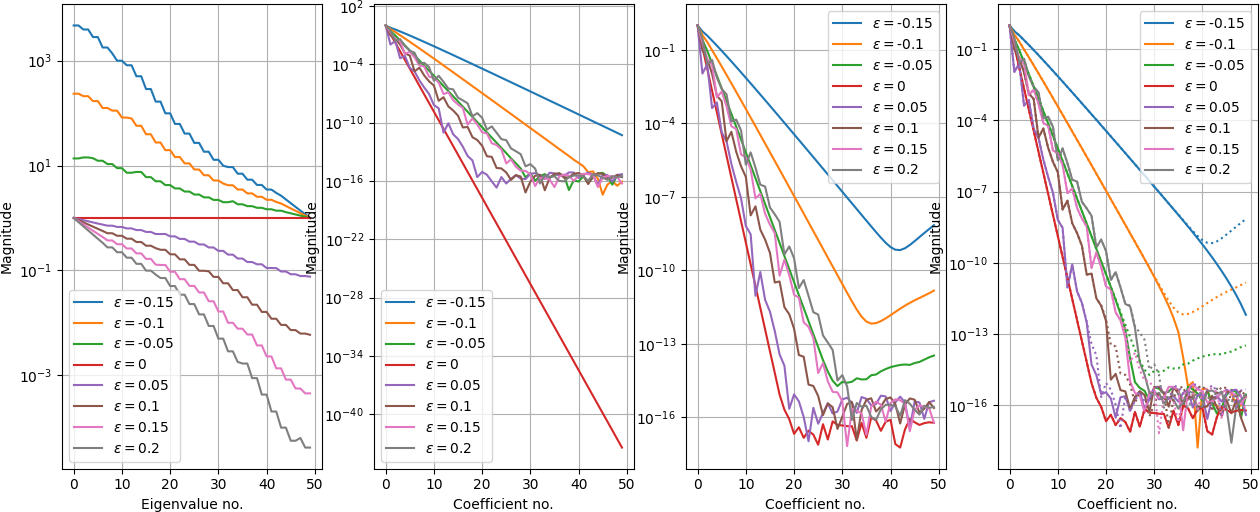
\includegraphics[width=\textwidth]{dat/projection_different_eps.png}
\caption{(a) Eigenvalues of projection operator for different $\varepsilon$; (b) Projection of clean data; (c) Projection of polluted data; (d) Projection of polluted data with small steps and thresholding}
\end{figure}

To inspect the behavior of the projection operator more closely, let us consider projection of a series which coefficients are given by $a_i = \exp\of{-100i}$. The results of projection with different $\varepsilon$ are given in Figure~\ref{fig:projection} (b) and, at the first glance, do not indicate of any instabilities. However, this is likely due to coefficients $a_i$ decaying very fast. Indeed, if we add a random noise to coefficients $a_i$ then the projection results seem to stay stable only if $\varepsilon > 0$ while for $\varepsilon < 0$ high-order coefficients growing uncontrollably (see Figure~\ref{fig:projection} (c)). 

A possible fix could be to use multiple small projection steps with zeroing all coefficients below a chosen threshold after each sub-step. The example of such a strategy is given in  Figure~\ref{fig:projection} (d) where a target relative change $\varepsilon_0 = 0.001$ was used (that is, the number of sub-steps and their size are chosen as $m = \text{ceil}\of{\frac{\log\of{1+\varepsilon}}{\log\of{1+\varepsilon_0}}}$ and $\tilde{\varepsilon} = \sqrt[n]{1+\varepsilon} - 1$). This strategy produces almost identical results as in the case of one full step and does not result in an uncontrollable growth of high-order coefficients for $\varepsilon < 0$. However, it is unclear whether there are any growing instabilities in the low-order part of the spectrum which are not seen due to large values of the coefficients there.


\begin{figure}[H]
\centering
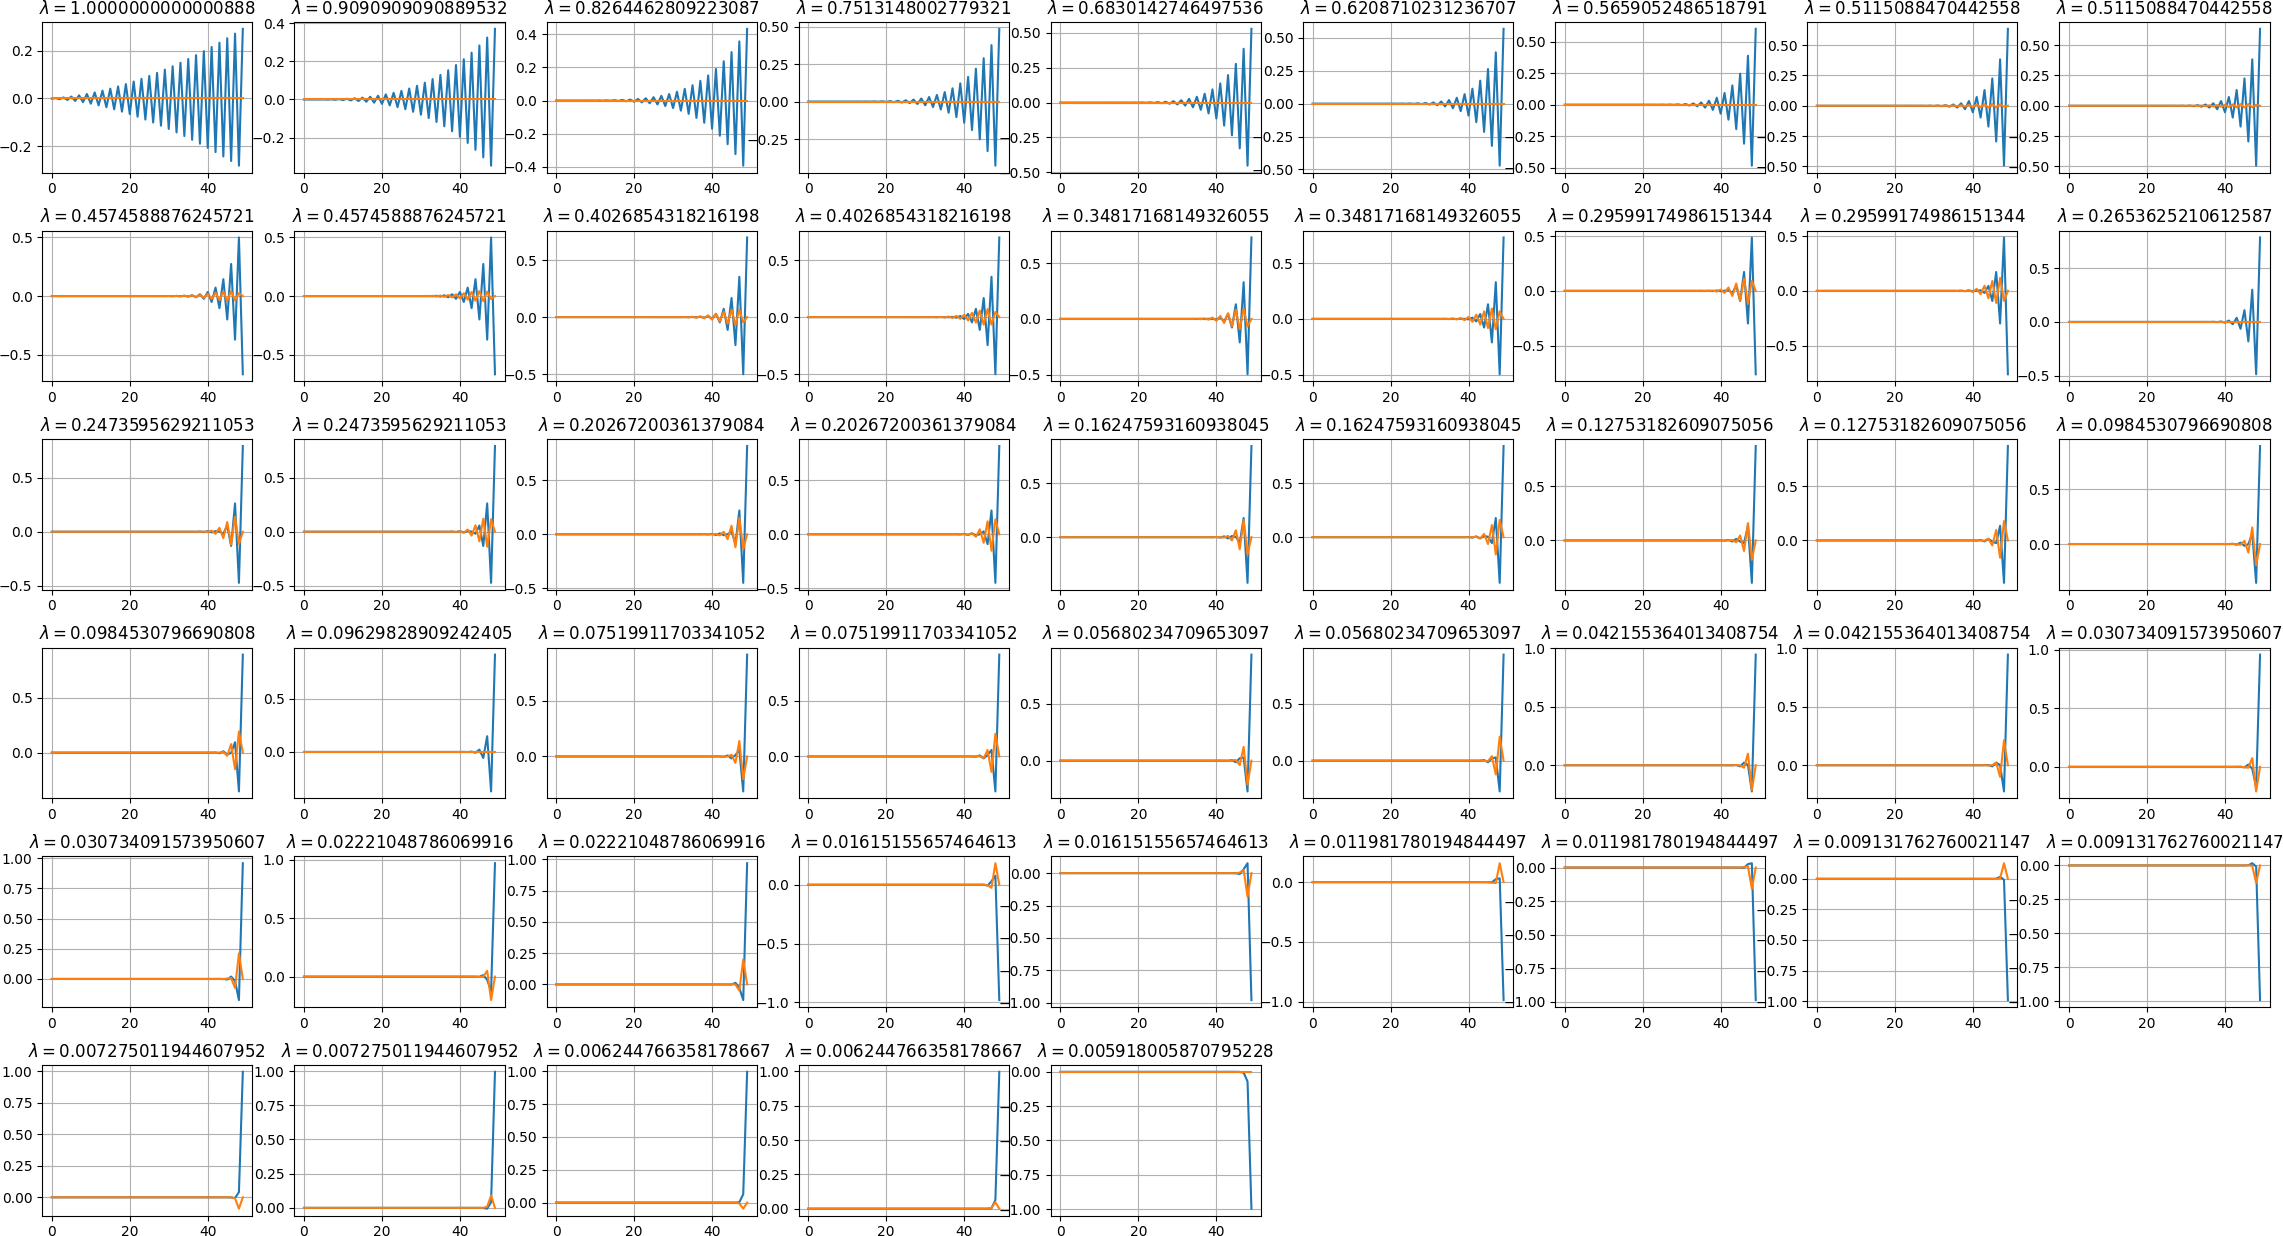
\includegraphics[width=1.2\textwidth]{dat/projection_pos_eigs.png}
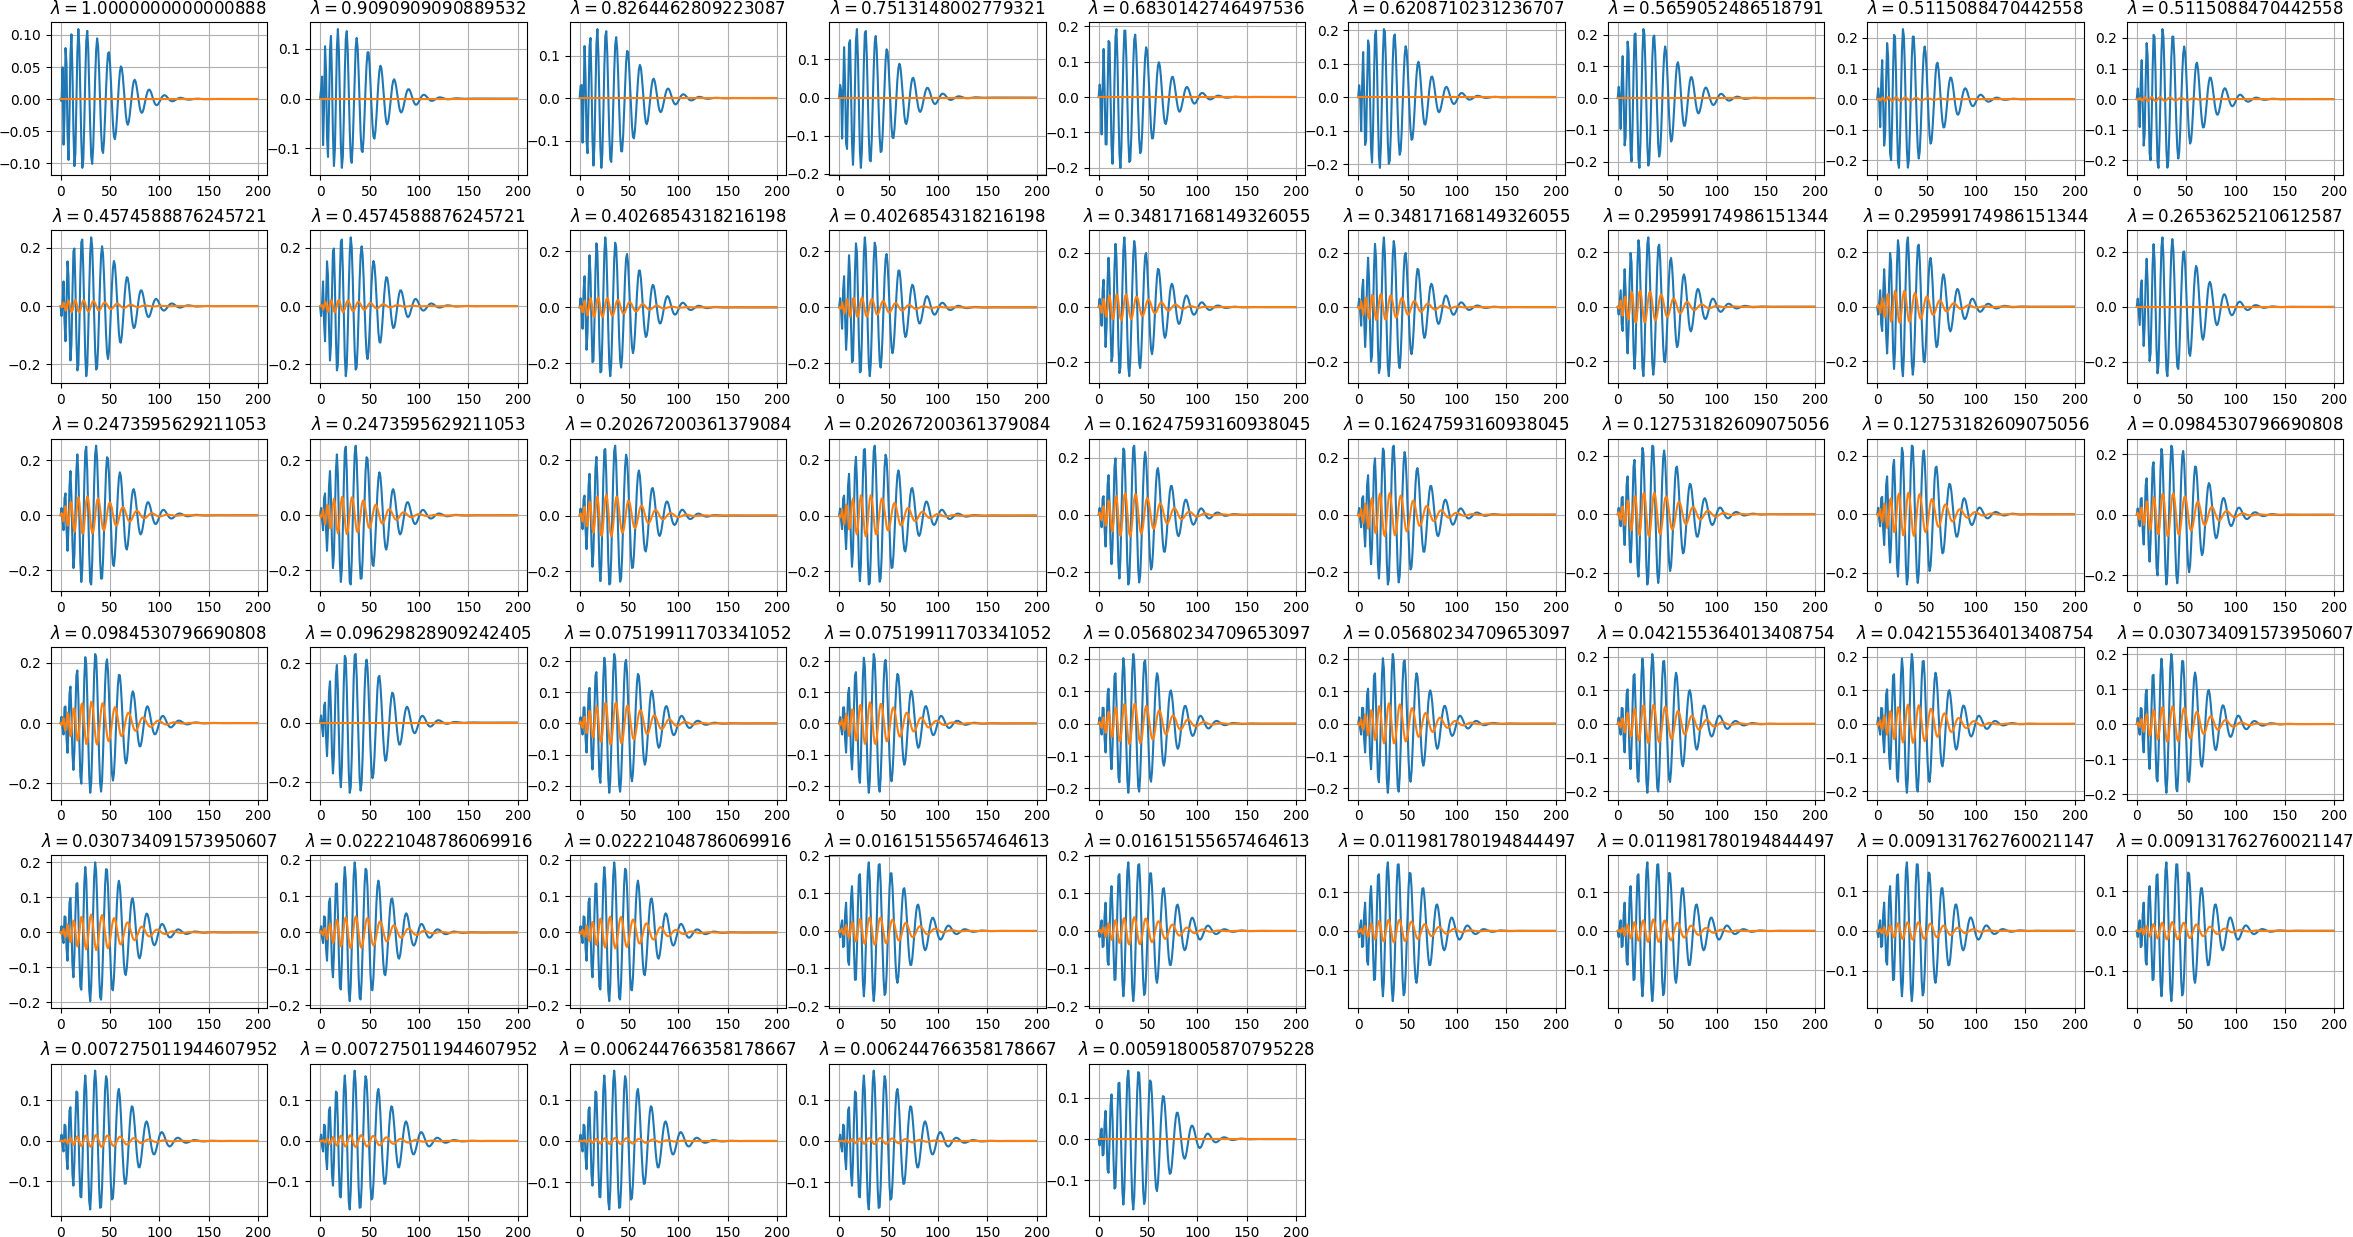
\includegraphics[width=1.2\textwidth]{dat/projection_pos_eigs_visual.png}
\caption{Eigenvectors (top) and their visualization (bottom) for $\varepsilon = 0.1$}
\end{figure}

\begin{figure}[H]
\centering
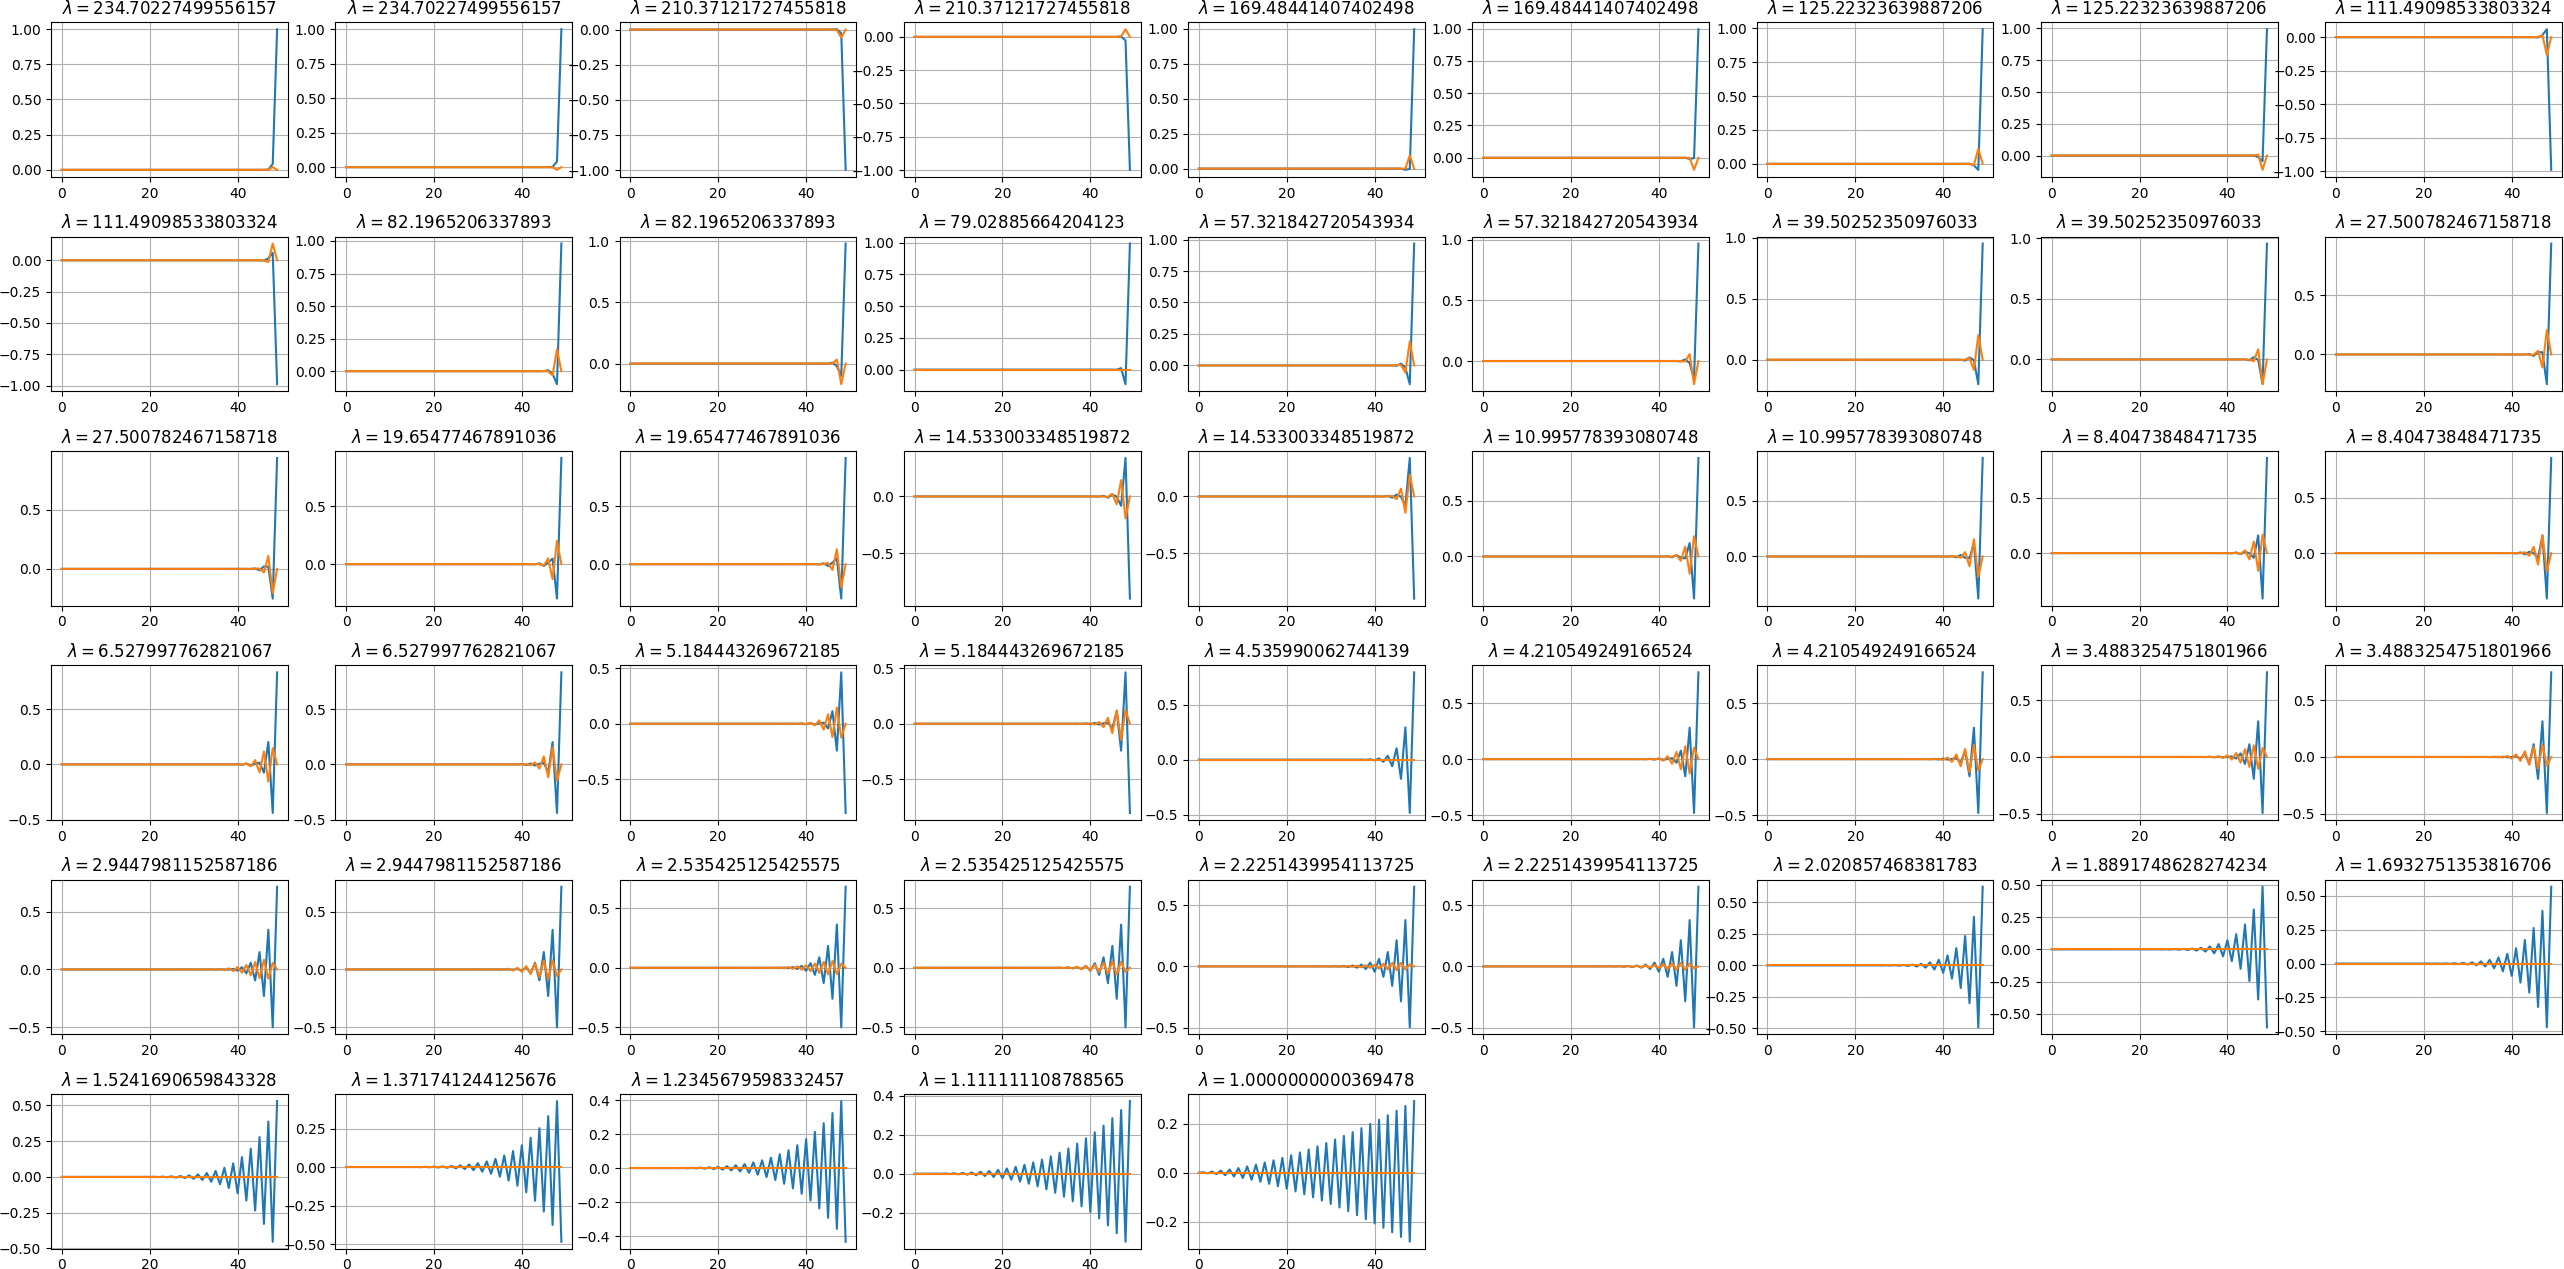
\includegraphics[width=1.2\textwidth]{dat/projection_neg_eigs.png}
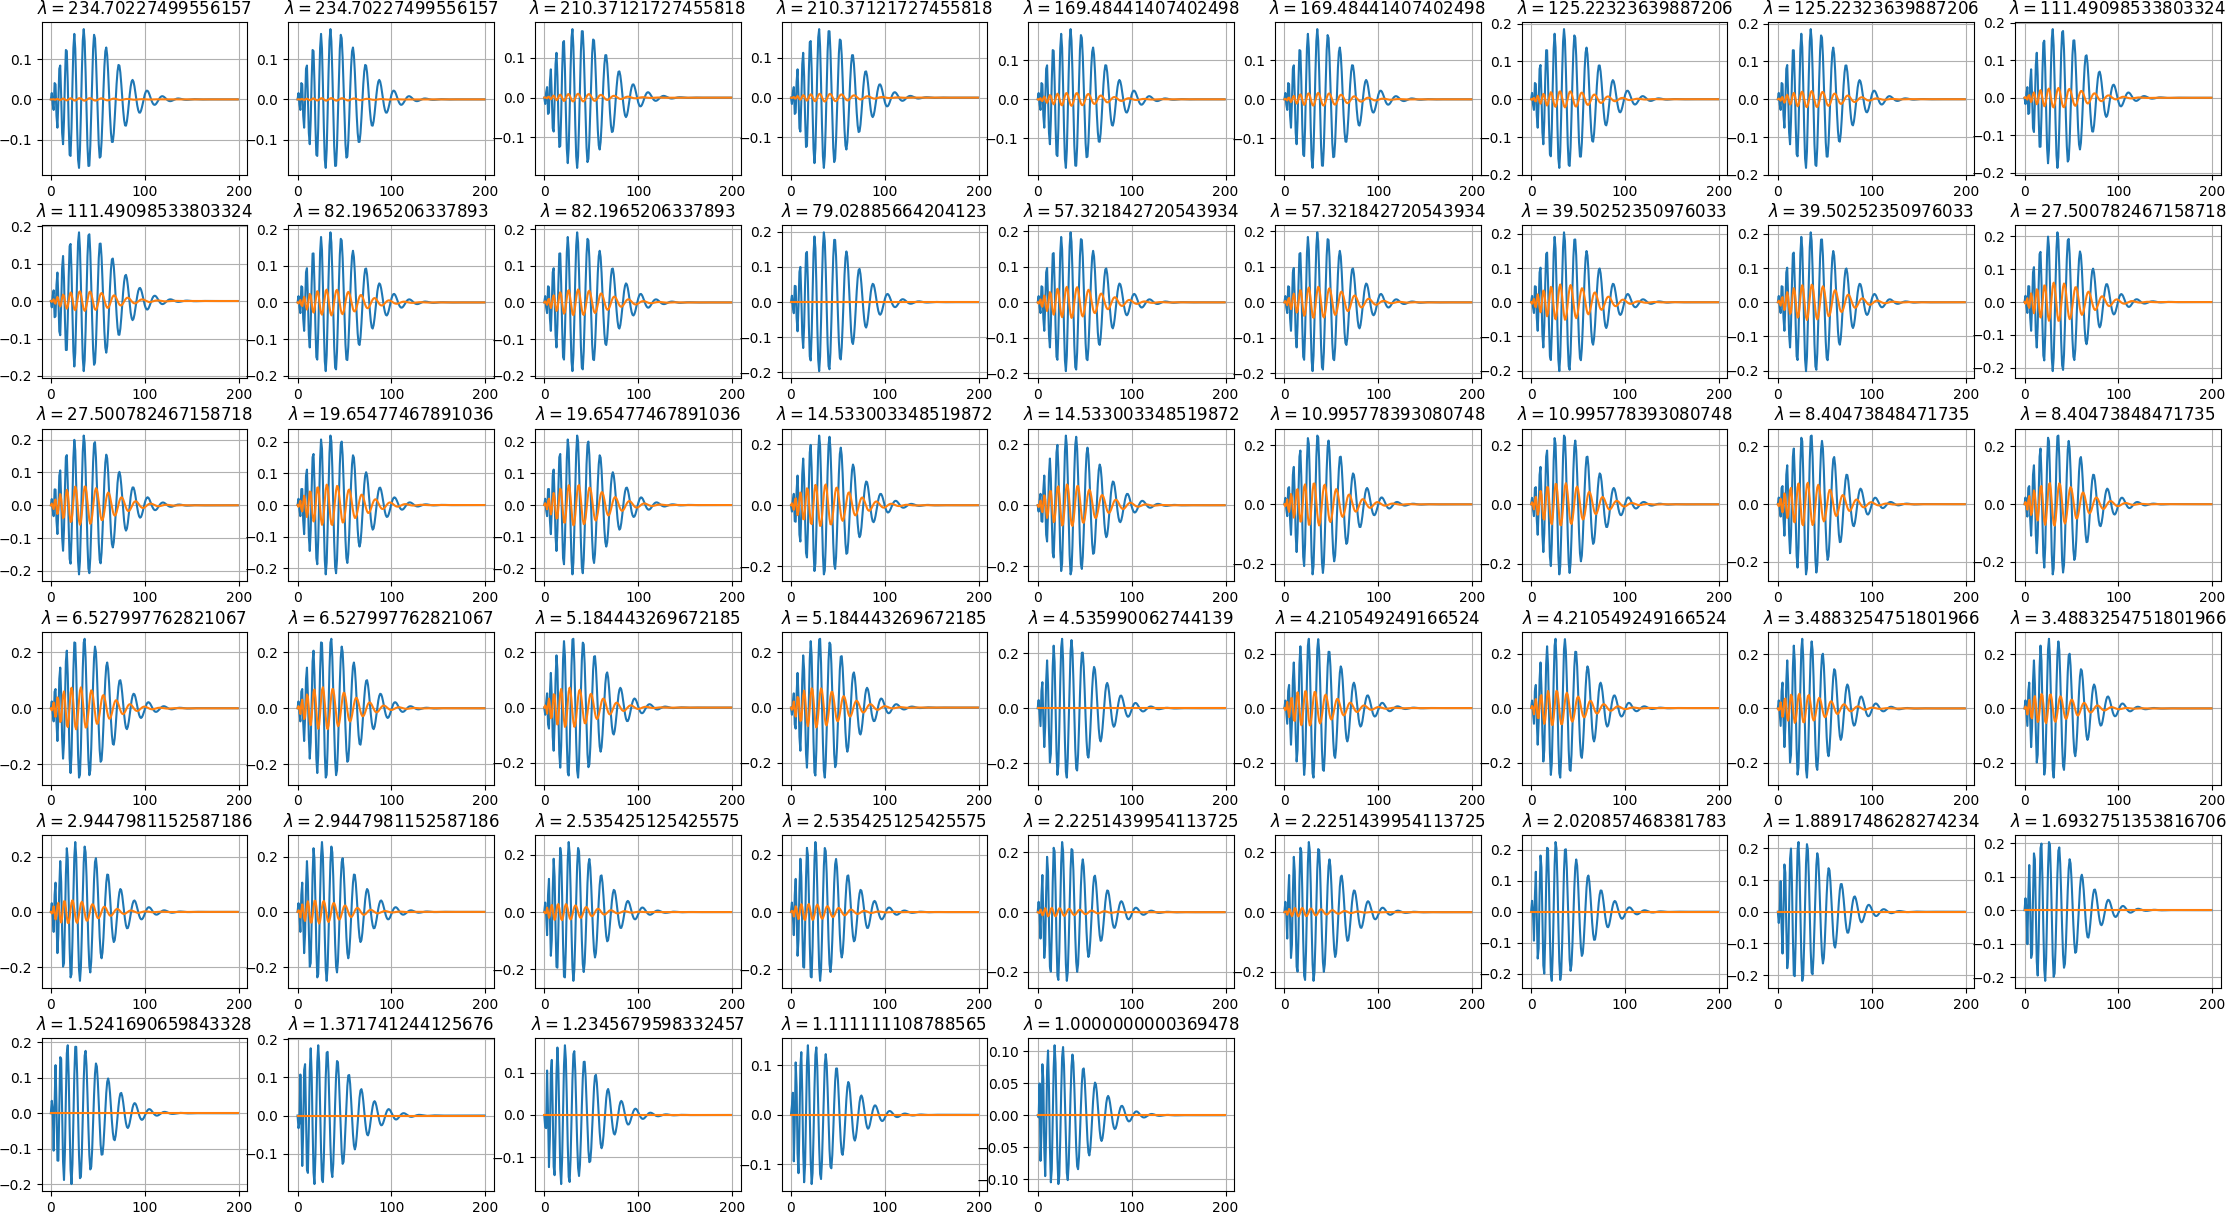
\includegraphics[width=1.2\textwidth]{dat/projection_neg_eigs_visual.png}
\caption{Eigenvectors (top) and their visualization (bottom) for $\varepsilon = -0.1$}
\end{figure}

\clearpage
\section{Advection term (initial poor attempt)}
Advection (acceleration) term
\begin{align*}
\partial_t f + \vect{E}\cdot \nabla_{\vect{v}} f = 0
\end{align*}

In spherical coordinates
\begin{align*}
\nabla_{\vect{v}} 
= \vrunit \frac{\partial}{\partial \vr}
+ \vthetaunit \frac{1}{\vr} \frac{\partial}{\partial \vtheta}
+ \vphiunit \frac{1}{\vr \sin\of{\vtheta}} \frac{\partial}{\partial \vphi}
\end{align*}

\begin{align*}
\vect{E} 
= E \hat{\vect{z}} 
= E \left( \cos\of{\vtheta} \vrunit - \sin\of{\vtheta} \vthetaunit \right)
\end{align*}


\begin{align*}
\vect{E}\cdot \nabla_{\vect{v}} f
= E 
\left( \cos\of{\vtheta} \frac{\partial f}{\partial \vr} 
- \sin\of{\vtheta} \frac{1}{\vr} \frac{\partial f}{\partial \vtheta} \right)
\end{align*}

Expansion in terms of Maxwell polynomials and spherical harmonics
\begin{align*}
f = A 
\exp\of{-\left(\frac{\vr}{\vth}\right)^2} 
\sum_{klm} a_{klm} P_k\of{\textstyle\frac{v}{\vth}} Y_{lm}\of{\vtheta,\vphi}
\end{align*}

Differentiation and lifting matrices
\begin{align*}
P^\prime_k\of{x} &= \sum_{j=0}^{N_r} d_{jk} P_j\of{x}
&
&\rightarrow \quad
\sum_{k=0}^{N_r} a_k P^\prime_k\of{x} 
= \sum_{k=0}^{N_r} \sum_{j=0}^{N_r} d_{jk} a_k P_j\of{x}
= \sum_{j=0}^{N_r} \left( \sum_{k=0}^{N_r} d_{jk} a_k \right) P_j\of{x}
\\
x P_k\of{x} &= \sum_{j=0}^{N_r} l_{jk} P_k\of{x}
&
&\rightarrow \quad
\sum_{k=0}^{N_r} a_k x P_k\of{x} 
= \sum_{k=0}^{N_r} \sum_{j=0}^{N_r} l_{jk} a_k P_j\of{x}
= \sum_{j=0}^{N_r} \left( \sum_{k=0}^{N_r} l_{jk} a_k \right) P_j\of{x}
\end{align*}
where $d_{jk}$ and $l_{jk}$ are calculated from recursive coefficients generating polynomials

\begin{align*}
\left( e^{-x^2} P_k\of{x} \right)^\prime
= - 2 x e^{-x^2} P_k\of{x} + e^{-x^2} P^\prime_k\of{x}
&= e^{-x^2} \sum_{j=0}^{N_r} \left( d_{jk} - 2 l_{jk} \right)P_j\of{x}
\\
&= e^{-x^2} \sum_{j=0}^{N_r} g_{jk} P_j\of{x}
\end{align*}

\begin{align*}
\frac{\partial f}{\partial v}
=
\frac{1}{\vth}
A \exp\of{-\left(\frac{\vr}{\vth}\right)^2} 
\sum_{lm} \sum_{j=0}^{N_r} 
\left(\sum_{k=0}^{N_r} g_{jk} a_{klm} \right) 
P_j\of{\frac{\vr}{\vth}} Y_{lm}\of{\vtheta,\vphi}
\end{align*}

\begin{align*}
\frac{1}{\vr}\frac{\partial f}{\partial \vtheta}
=
\frac{1}{\vr} A \exp\of{-\left(\frac{\vr}{\vth}\right)^2} 
\sum_{klm} a_{klm} P_k\of{\frac{\vr}{\vth}} 
\frac{\partial}{\partial \vtheta} Y_{lm}\of{\vtheta,\vphi}
\end{align*}

\begin{multline*}
\myint \cos\of{\vtheta} \frac{\partial f}{\partial \vr} P_p\of{\frac{\vr}{\vth}} Y_{qs}\of{\vtheta,\vphi} \vr^2 \diff{\vr} \diff{\vomega}
\\
=
\frac{1}{\vth}
A \sum_{lm} \sum_{j=0}^{N_r} \left(\sum_{k=0}^{N_r} g_{jk} a_{klm} \right) 
\left(
\int 
\exp\of{-\left(\frac{\vr}{\vth}\right)^2} P_j\of{\frac{v}{\vth}} P_p\of{\frac{\vr}{\vth}} \vr^2 
\diff{v}
\right)
\\
\times
\left(
\int
\cos\of{\vtheta} 
Y_{lm}\of{\vtheta,\vphi}
Y_{qs}\of{\vtheta,\vphi}
\diff{\vomega}
\right)
\\
=
\vth^2
A \sum_{lm} \sum_{j=0}^{N_r} \left(\sum_{k=0}^{N_r} g_{jk} a_{klm} \right) 
M_{p} \delta_{j,p}
\Psi_{lmqs}
=
\vth^2
A \sum_{lm} \left(\sum_{k=0}^{N_r} g_{pk} a_{klm} \right) 
M_{p}
\Psi_{lmqs}
\end{multline*}

\begin{multline*}
\myint \sin\of{\vtheta} \frac{1}{\vr} \frac{\partial f}{\partial \vtheta} P_p\of{\frac{v}{\vth}} Y_{qs}\of{\vtheta,\vphi} \vr^2 \diff{\vr} \diff{\vomega}
=
\\
A \sum_{lm} \sum_{j=0}^{N_r} \left(\sum_{k=0}^{N_r} g_{jk} a_{klm} \right) 
\left(
\int 
\exp\of{-\left(\frac{\vr}{\vth}\right)^2} P_j\of{\frac{\vr}{\vth}} P_p\of{\frac{\vr}{\vth}} \vr
\diff{\vr}
\right)
\\
\times
\left(
\int
\sin\of{\vtheta} 
Y_{qs}\of{\vtheta,\vphi}
\frac{\partial}{\partial \vtheta}
Y_{lm}\of{\vtheta,\vphi}
\diff{\vomega}
\right)
\end{multline*}

\begin{multline*}
\int 
\exp\of{-\left(\frac{\vr}{\vth}\right)^2} P_j\of{\frac{\vr}{\vth}} P_p\of{\frac{\vr}{\vth}} \vr
\diff{\vr}
=
\vth^2
\int 
e^{-x^2} P_j\of{x} P_p\of{x} x
\diff{x}
\\
=
-
\frac{\vth^2}{2}
\int 
x^2
\left(
e^{-x^2} P_j\of{x} P_p\of{x}
\right)'
\diff{x}
\\
=
-
\frac{\vth^2}{2}
\int 
x^2
e^{-x^2} 
\left(
-2x
P_j\of{x} P_p\of{x}
+
P^\prime_j\of{x} P_p\of{x}
+
P_j\of{x} P^\prime_p\of{x}
\right)
\diff{x}
\\
=
\frac{\vth^2}{2}
\int 
x^2
e^{-x^2} 
\left(
\sum_{k} 2l_{kj} P_k\of{x} P_p\of{x}
-
\sum_{k} d_{kj} P_k\of{x} P_p\of{x}
-
\sum_{k} d_{kp} P_j\of{x} P_k\of{x}
\right)
\diff{x}
\\
=
\frac{\vth^2}{2}
\left(
\sum_{k} 2l_{kj} \int x^2 e^{-x^2} P_k\of{x} P_p\of{x} \diff{x}
-
\sum_{k} d_{kj} \int x^2 e^{-x^2} P_k\of{x} P_p\of{x} \diff{x}
-
\sum_{k} d_{kp} \int x^2 e^{-x^2} P_j\of{x} P_k\of{x} \diff{x}
\right)
\\
=
-
\frac{\vth^2}{2}
\left(
\sum_{k} g_{kj} M_p \delta_{k,p}
+
\sum_{k} d_{kp} M_j \delta_{k,j} 
\right)
=
-
\frac{\vth^2}{2}
\left(
g_{pj} M_p
+
d_{jp} M_j
\right)
\end{multline*}

\begin{multline*}
\myint \sin\of{\vtheta} \frac{1}{\vr} \frac{\partial f}{\partial \vtheta} P_p\of{\textstyle\frac{\vr}{\vth}} Y_{qs}\of{\vtheta,\vphi} \vr^2 \diff{\vr} \diff{\vomega}
=
\\
-
\frac{\vth^2}{2}
A \sum_{lm} \sum_{j=0}^{N_r} \left(\sum_{k=0}^{N_r} g_{jk} a_{klm} \right) 
\left(
g_{pj} M_p
+
d_{jp} M_j
\right)
\Phi_{lmqs}
\end{multline*}

\begin{multline*}
\myint \vect{E}\cdot \nabla_{\vect{v}} f P_p\of{\textstyle\frac{\vr}{\vth}} Y_{qs}\of{\theta,\phi} \vr^2 \diff{\vr} \diff{\vomega}
\\
=
E
\vth^2
A \sum_{lm} \left(\sum_{k=0}^{N_r} g_{pk} a_{klm} \right) 
M_{p}
\Psi_{lmqs}
+
\frac{\vth^2}{2}
A \sum_{lm} \sum_{j=0}^{N_r} \left(\sum_{k=0}^{N_r} g_{jk} a_{klm} \right) 
\left(
g_{pj} M_p
+
d_{jp} M_j
\right)
\Phi_{lmqs}
\\
=
E
\sum_{klm}
\epsilon_{pqsklm} a_{klm}
\end{multline*}

\begin{align*}
\epsilon_{pqsklm} =
\vth^2 A 
\left(
g_{pk} M_{p} \Psi_{lmqs}
+
\frac{1}{2}
\sum_{j=0}^{N_r} g_{jk} 
\left(
g_{pj} M_p
+
d_{jp} M_j
\right)
\Phi_{lmqs}
\right)
\end{align*}


Let the polynomials on the radial direction is defined as, 
\begin{align}
	P_{kl} = b_k(x) x^l
\end{align} where $b_k$ be the $k^{th}$ bspline polynomial. 

For expansion using bspline polynomials in the radial direction we can write, 
\begin{align}
f(\vect{v}) &= \sum_{klm} a_{klm} P_{kl}\of{\textstyle\frac{v}{\vth}} Y_{lm}\of{\vtheta,\vphi}\\
\partial_v f &= \frac{1}{\vth} \sum_{klm} a_{klm} P^\prime_{kl}\of{\textstyle\frac{v}{\vth}} Y_{lm}\of{\vtheta,\vphi}\\
\frac{1}{v}\partial_{v_\theta} f &= \sum_{klm} a_{klm} P_{kl}\of{\textstyle\frac{v}{\vth}} \partial_{v_\theta} Y_{lm}\of{\vtheta,\vphi}
\end{align}

\begin{multline}
\myint \myint \cos\of{\vtheta} \frac{\partial f}{\partial \vr} P_{pq}\of{\frac{\vr}{\vth}} Y_{qs}\of{\vtheta,\vphi} \vr^2 \diff{\vr} \diff{\vomega}= \\
\sum_{klm} a_{klm} \myint \myint \frac{v^2}{\vth}  P^\prime_{kl}\of{\frac{\vr}{\vth}} P_{pq}\of{\frac{\vr}{\vth}} \cos\of{\vtheta} Y_{lm}\of{\vtheta,\vphi} Y_{qs}\of{\vtheta,\vphi} \diff{v}\diff{v_\omega} =\\
\sum_{klm} a_{klm} \myint \frac{v^2}{\vth}  P^\prime_{kl}\of{\frac{\vr}{\vth}} P_{pq}\of{\frac{\vr}{\vth}} \diff{v} \Psi_{lmqs}
\end{multline}

\begin{multline*}
\myint \myint \sin\of{\vtheta} \frac{1}{\vr} \frac{\partial f}{\partial \vtheta} P_{pq}\of{\textstyle\frac{\vr}{\vth}} Y_{qs}\of{\vtheta,\vphi} \vr^2 \diff{\vr} \diff{\vomega} = \\
\sin\of{\vtheta}\left(\sum_{klm} a_{klm} P_{kl}\of{\textstyle\frac{v}{\vth}} \partial_{v_\theta} Y_{lm}\of{\vtheta,\vphi} \right) P_{pq}\of{\textstyle\frac{\vr}{\vth}} Y_{qs}\of{\vtheta,\vphi} \vr \diff{\vr} \diff{\vomega} = \\
\sum_{klm} a_{klm} \myint v P_{pq}\of{\textstyle\frac{v}{\vth}} P_{kl}\of{\textstyle\frac{v}{\vth}} dv \myint \sin\of{\vtheta} \partial_{v_\theta} Y_{lm}\of{\vtheta,\vphi}  Y_{qs}\of{\vtheta,\vphi} \diff{v_{\omega}} = \\
\sum_{klm} a_{klm} \myint v P_{pq}\of{\textstyle\frac{v}{\vth}} P_{kl}\of{\textstyle\frac{v}{\vth}} dv \phi_{lmqs}
\end{multline*}


\subsection{Case of Laguerre polynomials (fancy attempt)}
An attempt to compute advection operator analytically in the case of Laguerre polynomials. There are some mistakes early on that propagates throughout the derivations. However, it still gives an overall idea how to proceed. Maybe will revisit later.

\begin{align*}
\lp{l}{0}\of{x} &= 1 \\
\lp{l}{1}\of{x} &= 1 + l - x \\
\lp{l}{k+1}\of{x} &= \frac{(2k+1+l-x) \lp{l}{k}\of{x} - (k+l) \lp{l}{k-1}\of{x}}{k+1}
\end{align*}

\begin{align*}
\myint_0^\infty e^{-x} x^l \lp{l}{k}\of{x} \lp{l}{p}\of{x} \diff{x} = \frac{\Gamma\of{p + l + 1}}{n!} \delta_{k,p}
\end{align*}

\begin{align*}
\lph{l}{k} = \lp{l+1/2}{k}
\end{align*}

\begin{align*}
\Phi_{kl}\of{x} &= e^{-x^2} x^l \lph{l}{k}\of{x^2} \\
\Psi_{pq}\of{x} &= x^q \lph{q}{p}\of{x^2} 
\end{align*}

\begin{align*}
\myint_0^\infty \Phi_{kq}\of{x} \Psi_{pq}\of{x} x^2 \diff{x} 
&= \myint_0^\infty e^{-x^2} x^{2q+2}\lph{q}{k}\of{x^2} \lph{q}{p}\of{x^2} \diff{x}
\\
&= \frac12 \myint_0^\infty e^{-y} y^{q+1/2}\lph{q}{k}\of{y} \lph{q}{p}\of{y} \diff{x}
\\
&= N_{p,q} \delta_{k,p}
\end{align*}

Useful formulae
\begin{align*}
\lph{l+1}{k} \of{x^2} &= \sum_{j=0}^{k} \lph{l}{j}\of{x^2}
\\
\lph{l}{k} \of{x^2} &= \lph{l+1}{k} \of{x^2} - \lph{l+1}{k-1} \of{x^2}
\\
x^2 \lph{l+1}{k} \of{x^2} 
&= (k+l+3/2) \lph{l}{k}\of{x^2} - (k+1) \lph{l}{k+1}\of{x^2}
\\
%x^2 L^{(l+2)}_k \of{x^2} 
%&= (k+l+2) \lp{l+1}{k}\of{x^2} - (k+1) \lp{l+1}{k+1}\of{x^2}
%\\
%&= (k+l+2) \sum_{j=0}^{k} \lp{l}{j}\of{x^2} - (k+1) \sum_{j=0}^{k+1} \lp{l}{j}\of{x^2}
%\\
%&= (l+1) \sum_{j=0}^{k} \lp{l}{j}\of{x^2} - (k+1) \lp{l}{k+1}\of{x^2}
%\\
\frac{d}{dx^2} \lph{l}{k} \of{x^2} &= - \lph{l+1}{k-1} \of{x^2}
\\
\frac{d}{dx} \lph{l}{k} \of{x^2} 
&= 2 x \frac{d}{dx^2} \lph{l}{k}\of{x^2} = - 2 x \lph{l+1}{k-1}\of{x^2}
%\\
%x \frac{d}{dx} \lp{l+1}{k} \of{x^2} 
%&= 2 x^2 \frac{d}{dx^2} \lp{l+1}{k}\of{x^2} = - 2 x^2 \lp{l+2}{k-1}\of{x^2}
%\\
%&= -2(l+1) \sum_{j=0}^{k-1} \lp{l}{j}\of{x^2} 
%+ 2 k \lp{l}{k}\of{x^2}
\end{align*}

%\begin{align*}
%\frac{d}{dx}\Phi_{k,q+1}\of{x} 
%&= - 2 e^{-x^2} x^{q+2} L^{(q+1)}_k\of{x^2}
%+ (q+1) e^{-x^2} x^{q} L^{(q+1)}_k\of{x^2}
%+ e^{-x^2} x^{q+1} \frac{d}{dx} L^{(q+1)}_k\of{x^2}
%\\
%&= e^{-x^2} x^{q} \Big( 
%- 2 (k+q+1) L^{(q)}_k\of{x^2} + 2 (k+1) L^{(q)}_{k+1}\of{x^2} 
%\\&
%+ (q+1) \sum_{j=0}^{k} L^{(q)}_j\of{x^2}
%- 2(q+1) \sum_{j=0}^{k-1} \lp{q}{j}\of{x^2} 
%+ 2 k \lp{q}{k}\of{x^2}
%\Big)
%\\
%&= e^{-x^2} x^{q} \Big( 
%2 (k+1) L^{(q)}_{k+1}\of{x^2} 
%- (q+1) \sum_{j=0}^{k} \lp{q}{j}\of{x^2} 
%\Big)
%\\
%&= 2 (k+1) \Phi_{k+1,q}\of{x}
%- (q+1) \sum_{j=0}^{k} \Phi_{j,q}\of{x} 
%\end{align*}

%\begin{align*}
%\myint_0^\infty \Psi_{p,q}\of{x} \frac{d}{dx}\Phi_{k,q+1}\of{x}  x^2 \diff{x}
%&= 2 (k+1) N_{p,q} \delta_{p,k+1}  - (q+1) \sum_{j=0}^{k} N_{p,q} \delta_{p,j} 
%\\
%&= N_{p,q} \sum_{j=0}^{k+1} \Omega \delta_{p,j} 
%\end{align*}

\begin{multline*}
\tfun{q}{p}\of{x} \frac{d}{dx} \bfun{q+1}{k}\of{x} 
= x^q \lph{q}{p} \frac{d}{dx} e^{-x^2} x^{q+1} \lph{q+1}{k}
\\
= x^q \lph{q}{p} \left( 
- 2 e^{-x^2} x^{q+2} \lph{q+1}{k}\of{x^2}
+ (q+1) e^{-x^2} x^{q} \lph{q+1}{k}\of{x^2}
- 2 e^{-x^2} x^{q+2} \lph{q+2}{k-1}\of{x^2}
\right)
\\ 
= 
-2 x^q \lph{q}{p} e^{-x^2} x^q \left( (k+q+3/2) \lph{q}{k} - (k+1) \lph{q}{k+1} \right) 
\\
+ (q+1) x^q \lph{q}{p} e^{-x^2} x^q \sum_{j=0}^{k} \lph{q}{j}
-2 x^{q+1} \left( \lph{q+1}{p} - \lph{q+1}{p-1} \right) e^{-x^2} x^{q+1} \sum_{j=0}^{k-1} \lph{q+1}{j}
\\ 
= 
-2 \tfun{q}{p} \left( (k+q+3/2) \bfun{q}{k} - (k+1) \bfun{q}{k+1} \right) 
+ (q+1)\tfun{q}{p} \sum_{j=0}^{k} \bfun{q}{j}
-2\left( \tfun{q+1}{p} - \tfun{q+1}{p-1} \right) \sum_{j=0}^{k-1} \bfun{q+1}{j}
\end{multline*}


\begin{multline*}
\myint_0^\infty \tfun{q}{p}\of{x} \frac{d}{dx} \bfun{q+1}{k}\of{x} 
= 
-2 \nfun{q}{p} \left( (k+q+3/2)\delta_{p,k} - (k+1) \delta_{p,k+1} \right) 
+ (q+1)\nfun{q}{p} \sum_{j=0}^{k} \delta_{p,j}
\\
-2\left( \nfun{q+1}{p} \sum_{j=0}^{k-1} \delta_{p,j} - \nfun{q+1}{p-1} \sum_{j=0}^{k-1} \delta_{p-1,j} \right)  
\end{multline*}

Warning: what's below is not correct (forgot 1/2 in Laguerre index)
\begin{align*}
\Phi_{k,q+1}\of{x} \frac{d}{dx}\Psi_{p,q}\of{x} 
&= 
e^{-x^2} x^{q+1} L^{(q+1)}_k\of{x^2}
\left(
q x^{q-1} L^{(q)}_p\of{x^2}
+ x^{q} \frac{d}{dx} L^{(q)}_p\of{x^2}
\right)
\\
&= e^{-x^2} x^{q} \sum_{j=0}^{k} \lp{q}{j}\of{x^2} q x^{q} L^{(q)}_p\of{x^2}
- \Phi_{k,q+1}\of{x} 2 x^{q+1} L^{(q+1)}_{p-1}\of{x^2}
\\
&= q \sum_{j=0}^{k} \Phi_{j,q}\of{x} \Psi_{p,q}\of{x}
- 2\Phi_{k,q+1}\of{x} \Psi_{p-1,q+1}\of{x}
\end{align*}

\begin{align*}
\myint_0^\infty \Phi_{k,q+1}\of{x} \frac{d}{dx}\Psi_{p,q}\of{x} x^2 \diff{x}
&= q \sum_{j=0}^{k} N_{p,q} \delta_{p,j} 
- 2 N_{p,q+1} \delta_{p-1,k} 
\\
&= q \sum_{j=0}^{k} N_{p,q} \delta_{p,j} 
- 2 N_{p,q+1} \delta_{p,k+1} 
\end{align*}

\begin{align*}
\Phi_{k, q-1}\of{x} \frac{d}{dx}\Psi_{pq}\of{x}
&= e^{-x^2} x^{q-1} \lp{q-1}{k}\of{x^2} \frac{d}{dx} x^{q} \lp{q}{p}\of{x^2}
\\
&= e^{-x^2} x^{q-1} \lp{q-1}{k}\of{x^2} 
\left(
q x^{q-1} L^{(q)}_p\of{x^2}
+ x^{q} \frac{d}{dx} L^{(q)}_p\of{x^2}
\right)
\\
&= q \Phi_{k, q-1}\of{x} \sum_{j=0}^p \Psi_{j,q-1}\of{x}
- 2 e^{-x^2} x^{q-1} \lp{q-1}{k}\of{x^2}  x^{q+1} \lp{q+1}{p-1}\of{x^2}
\\
&= q \Phi_{k, q-1}\of{x} \sum_{j=0}^p \Psi_{j,q-1}\of{x}
- 2 e^{-x^2} x^{q} \left( \lp{q}{k}\of{x^2} - \lp{q}{k-1}\of{x^2}\right)  x^{q} \sum_{j=0}^{p-1}\lp{q}{j}\of{x^2}
\\
&= q \sum_{j=0}^p \Phi_{k, q-1}\of{x} \Psi_{j,q-1}\of{x}
- 2 \sum_{j=0}^{p-1} \left( \Phi_{k,q}\of{x^2} - \Phi_{k-1,q}\of{x^2}\right) \Psi_{j,q}\of{x^2}
\end{align*}

\begin{align*}
\myint_0^\infty \Phi_{k, q-1}\of{x} \frac{d}{dx}\Psi_{pq}\of{x} x^2 \diff{x}
&= q \sum_{j=0}^{p} N_{k,q-1} \delta_{k,j} 
- 2 \sum_{j=0}^{p-1} \left( N_{k,q} \delta_{k,j} - N_{k-1,q} \delta_{k-1,j}  \right)
\end{align*}

%\begin{multline*}
%\Psi_{pq}\of{x} \frac{d}{dx}\Phi_{k, q-1}\of{x} 
%= x^q \lp{q}{p}\of{x^2} \frac{d}{dx} e^{-x^2} x^{q-1} \lp{q-1}{k}\of{x^2}
%\\
%= x^q \lp{q}{p}\of{x^2} \left(
%- 2 e^{-x^2} x^{q} L^{(q-1)}_k\of{x^2}
%+ (q-1) e^{-x^2} x^{q-2} L^{(q-1)}_k\of{x^2}
%+ e^{-x^2} x^{q+1} \frac{d}{dx} L^{(q+1)}_k\of{x^2}
%\right)
%\\
%= - x^{q-1} \left( (p+q) \lp{q-1}{p} - (p+1) \lp{q-1}{p+1} \right)
%e^{-x^2} x^{q-1} L^{(q-1)}_k
%\\
%+ (q-1) x^{q-1} \sum_{j=0}^{p} \lp{q-1}{j} e^{-x^2} x^{q-1} \lp{q-1}{k} 
%- 2 x^q \lp{q}{p} e^{-x^2} x^q \lp{q}{k-1}
%\\
%= - (p+q) \tfun{q-1}{p} \bfun{q-1}{k} 
%+ (p+1) \tfun{q-1}{p+1} \bfun{q-1}{k}
%+ (q-1) \sum_{j=0}^{p} \tfun{q-1}{j} \bfun{q-1}{k} 
%- 2 \tfun{q}{p} \bfun{q}{k-1}
%\end{multline*}


\begin{multline*}
\Psi_{pq}\of{x} \frac{d}{dx}\Phi_{k, q-1}\of{x} 
= x^q \lp{q}{p}\of{x^2} \frac{d}{dx} e^{-x^2} x^{q-1} \lp{q-1}{k}\of{x^2}
\\
= x^q \lp{q}{p}\of{x^2} \left(
- 2 e^{-x^2} x^{q} L^{(q-1)}_k\of{x^2}
+ (q-1) e^{-x^2} x^{q-2} L^{(q-1)}_k\of{x^2}
+ e^{-x^2} x^{q+1} \frac{d}{dx} L^{(q+1)}_k\of{x^2}
\right)
\\
= - x^{q} \lp{q}{p} 
e^{-x^2} x^{q} \left( \lp{q}{k} - \lp{q}{k-1} \right)
+ (q-1) x^{q-1} \sum_{j=0}^{p} \lp{q-1}{j} e^{-x^2} x^{q-1} \lp{q-1}{k} 
- 2 x^q \lp{q}{p} e^{-x^2} x^q \lp{q}{k-1}
\\
= - \tfun{q}{p} \bfun{q}{k} 
+ \tfun{q}{p} \bfun{q}{k-1}
+ (q-1) \sum_{j=0}^{p} \tfun{q-1}{j} \bfun{q-1}{k} 
- 2 \tfun{q}{p} \bfun{q}{k-1}
\end{multline*}

\begin{multline*}
\myint_0^\infty \Psi_{pq}\of{x} \frac{d}{dx}\Phi_{k, q-1}\of{x} x^2 \diff{x}
= -  \nfun{q}{p} \delta_{p,k} 
- \nfun{q}{p} \delta_{p,k-1}
+ (q-1) \sum_{j=0}^{p} \nfun{q-1}{j} \delta_{j,k}
\end{multline*}


\end{document}
